% le caratteristiche richieste dall'università sono elencate qui: https://stem.elearning.unipd.it/mod/book/view.php?id=234&chapterid=46#modalita
% 12pt: font richiesto dall'università
% twoside: i margini interni ed esterni sono scambiati per le pagine "a sinistra" e "a destra"
% openright: i capitoli cominciano in pagine dispari ("a destra")
% extreport: supporta 12pt
\documentclass[12pt,a4paper,twoside]{extreport}

\usepackage[hidelinks]{hyperref}
\usepackage{amsmath}                            % per avere più controllo sulle equazioni 
\usepackage{csquotes}                           % per le citazioni
\usepackage{enumitem}                           % per avere più controllo sulle enumerazioni
\usepackage[
    a4paper,
    top=2cm,bottom=2cm,
    outer=2cm,inner=3cm,
    includeheadfoot
]{geometry}                                     % margini richiesti dall'università
\usepackage{graphicx}                           % per le immagini
\usepackage{minted}                             % per il codice con la colorazione della sintassi
\usepackage[a-1b]{pdfx}                         % formato richiesto dall'università
\usepackage[output-decimal-marker={,}]{siunitx} % per le unità di misura
\usepackage{subcaption}                         % per le sottodidascalie
\usepackage{svg}             
\usepackage{tabularx}
\usepackage{booktabs}
\usepackage[most]{tcolorbox}
\usepackage[italian]{babel}
\selectlanguage{italian}

\usepackage[backend=bibtex,style=ieee]{biblatex}
\bibliography{bibliografia.bib}

\usepackage{fontspec}
\setmainfont{Times New Roman} % carattere richiesto dall'università

\usepackage{tikz}
\usetikzlibrary{calc}
\usetikzlibrary{positioning}

\usepackage{amssymb}

\usepackage{setspace}
\onehalfspacing % interlinea richiesta dall'università

\setlength{\parindent}{0pt}

\newenvironment{sitemize}{
    \begin{list}{\labelitemi}{
        \setlength{\itemsep}{0pt}
        \setlength{\parskip}{0pt}
        \setlength{\parsep}{0.25em}
        \setlength{\topsep}{0.5em}
        \setlength{\leftmargin}{1em}
        \setlength{\labelwidth}{1em}
        \setlength{\labelsep}{0.5em}
    }
}{
    \end{list}
}

\newtcolorbox{note}{
    enhanced,
    breakable,
    colback=lightgray!20,
    colframe=gray!50,
    borderline west={2pt}{0pt}{gray!80},
    arc=0mm,
    boxrule=0mm,
    boxsep=2mm,
    left=6pt,
    right=6pt,
    fonttitle=\bfseries,
    fontupper=\small\color{black!80}
}

\def\defequal{\overset{\scriptscriptstyle\Delta}{=}}

\sloppy % per evitare che il testo in \verb finisca oltre i margini

% questi valori vengono usati nella composizione del frontespizio
\title{Modellazione e controllo laterale e longitudinale di un Boeing 747}
\author{Cuzzolin Matteo}
\date{21/07/2025}
\newcommand{\supervisor}{Prof. Zampieri Sandro}

\begin{document}
\allowdisplaybreaks
\pagenumbering{roman}
\pagestyle{empty} % per le prime pagine, non mostrare il numero di pagina

\newfontfamily\gyre{TeX Gyre Termes}

\begin{titlepage}
    % solo il frontespizio deve essere simmetrico rispetto ai margini interno ed esterno
    \newgeometry{hmargin=2.5cm,vmargin=2cm}
        \begin{figure}
            \centering
            \begin{subfigure}[b]{0.4\textwidth}
                
\includegraphics[width=\textwidth]{Immagini/logo_unipd}
            \end{subfigure}
            \hfill
            \begin{subfigure}[b]{0.3\textwidth}
                
\includegraphics[width=\textwidth]{Immagini/logo_dei}
            \end{subfigure}
        \end{figure}
    
        \vspace*{\stretch{0.5}}
    
        \begin{center}
            \makeatletter % serve per poter usare \@...

            % NOTA: il Times New Roman non supporta il maiuscoletto.
            {\gyre{\textsc{DIPARTIMENTO DI INGEGNERIA DELL'INFORMAZIONE}}\\}
            \vspace*{\stretch{0.1}}
            {\gyre{\textsc{CORSO DI LAUREA IN INGEGNERIA INFORMATICA}}\\}
    
            \vspace*{\stretch{0.5}}
            \LARGE
            \textbf{\@title}
    
            \vspace*{\stretch{1}}
            \normalsize
            \begin{tabular*}{\textwidth}{l @{\extracolsep{\fill}} r}
                \textbf{Relatore} & \textbf{Laureando} \\
                \supervisor       & \@author           \\
            \end{tabular*}
    
            \vspace*{\stretch{2}}
            {\gyre{\textsc{ANNO ACCADEMICO 2024-2025}}\\}
            \vspace*{\stretch{0.1}}
            Data di laurea \@date
        
            \makeatother % serve dopo \makeatletter
        \end{center}
    \restoregeometry
\end{titlepage}

\cleardoublepage

\abstract

Il Boeing 747, come molti velivoli moderni, è dotato di sistemi di controllo automatico progettati per mitigare gli effetti degli agenti atmosferici e per assistere il pilota nelle operazioni di volo.
Nella presente tesi viene sviluppato un modello matematico dell'aeromobile in grado di descriverne la dinamica e la cinematica, basato sulle equazioni del moto di un corpo rigido e sui dati del report tecnico NASA CR-2144.
Successivamente, vengono descritti due controllori: un autopilota, utilizzabile per assistere il pilota nel mantenimento di una determinata altitudine, e un controllore progettato per mitigare un fenomeno noto come "Dutch Roll", al quale sono particolarmente soggetti i velivoli di grandi dimensioni con ali a freccia positiva, come il Boeing 747.

% english
%The Boeing 747, like many modern aircraft, is equipped with automatic control systems designed to mitigate the effects of atmospheric disturbances and to assist the pilot during flight operations.
%In this thesis, a mathematical model of the aircraft is developed, capable of describing its dynamics and kinematics. The model is based on the equations of motion of a rigid body and parameterized using data from NASA technical report CR-2144.
%Subsequently, two controllers are described: an autopilot, which can be used to assist the pilot in maintaining a desired altitude, and a controller designed to mitigate a phenomenon known as Dutch Roll, to which large aircraft with swept wings, such as the Boeing 747, are particularly susceptible.

\cleardoublepage


\pagestyle{plain} % comincia a mostrare il numero di pagina
\setcounter{page}{1}
\tableofcontents

\cleardoublepage
\thispagestyle{empty}
\null
\newpage

\pagenumbering{arabic}

\chapter{Descrizione del Sistema Boeing 747}
Dopo l'introduzione del Boeing 707, uno dei primi jet commerciali ad entrare in servizio, Pan Am richiese un aereo circa due volte e mezzo più grande. Questa esigenza portò allo sviluppo del Boeing 747, che entrò in servizio nel 1970.

Per rispondere a questa esigenza, Boeing progettò un aereo a fusoliera larga con un'apertura alare di 65 metri ed una lunghezza di 70 metri, caratteristiche che gli valsero l'appellativo di "Jumbo Jet".
Il velivolo è spinto da quattro motori turboventola, che gli consentono di raggiungere una velocità massima di crociera di circa 1.040 km/h (Mach 0.85) ed un'autonomia di più di 13.000 km.

Grazie alla sua versatilità, il 747 ebbe un grande successo commerciale: nei 55 anni di produzione, Boeing ne costruì 1.574 esemplari. La maggior parte fu destinata al trasporto passeggeri, ma ne furono prodotte anche versioni cargo e militari.

\begin{figure}[H]
    \centering
    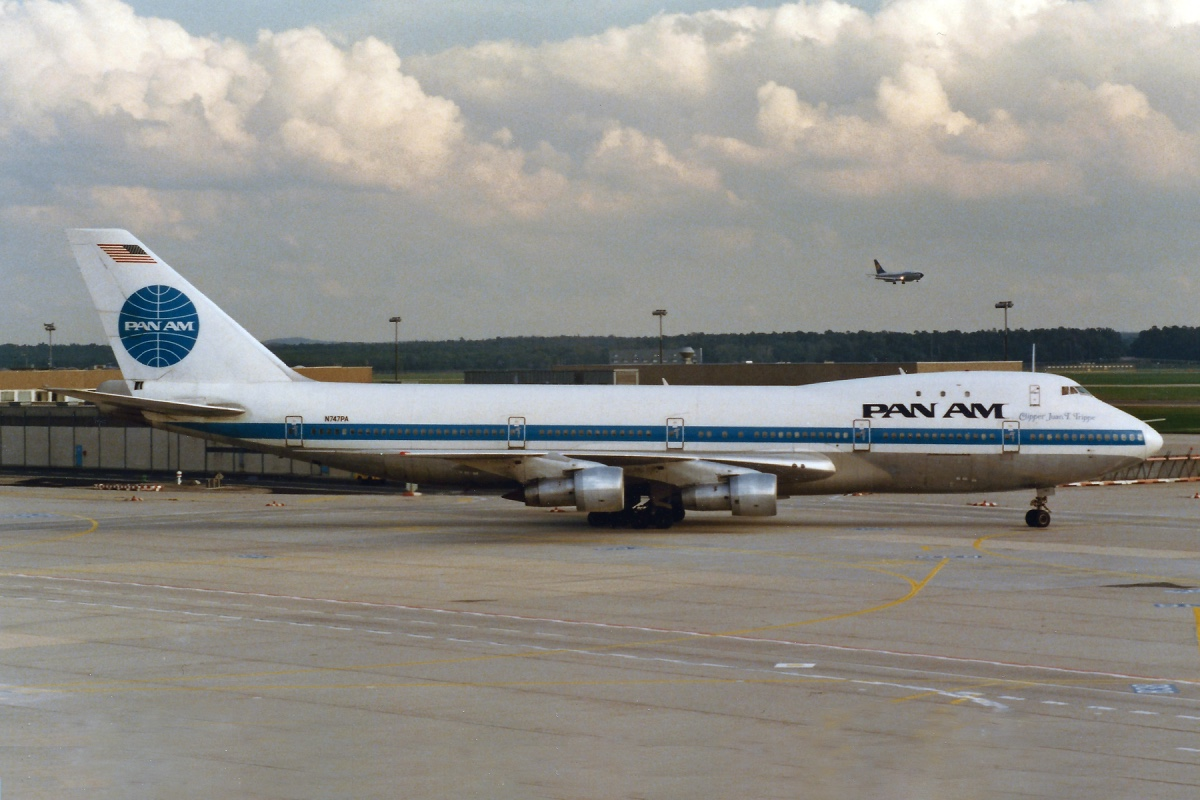
\includegraphics[width=0.65\linewidth]{Immagini/747.jpg}
    \caption{Un Boeing 747 di Pan Am \cite{747-image}}
\end{figure}

\newpage
\section{Sistemi di Riferimento}
Nella descrizione delle forze e delle quantità del velivolo è utile adottare diversi sistemi di riferimento standard utilizzati in aviazione.
Di seguito sono descritti i sistemi di riferimento utilizzati nel corso di questa tesi.

\subsection{Sistema di Riferimento NED}
La Terra sarà considerata un sistema di riferimento inerziale, trascurandone il suo movimento nello spazio in quanto esso è trascurabile rispetto a quello del velivolo.
Inoltre, la curvatura terrestre non verrà considerata: la superficie terrestre sarà approssimata ad un piano infinito.

Il sistema di riferimento $NED$ è un sistema di assi solidale con la Terra e, quindi, anch'esso approssimato come inerziale, con origine posta sulla superficie terrestre. Gli assi sono definiti come segue:
\begin{sitemize}
    \item Asse Down ($\hat{z}_{NED}$) è diretto verso il centro della Terra. Il verso positivo è concorde al verso del vettore di gravità.
    \item Asse North ($\hat{x}_{NED}$) definito dall'intersezione tra il piano orizzontale locale e il piano contenente l'asse di rotazione terrestre. Il verso positivo è orientato verso il nord geografico.
    \item Asse East ($\hat{y}_{NED}$) perpendicolare ai due assi già definiti con il verso positivo nella direzione di rotazione terrestre, in modo da ottenere una terna destrorsa.
\end{sitemize}

\begin{figure}[H]
    \centering
    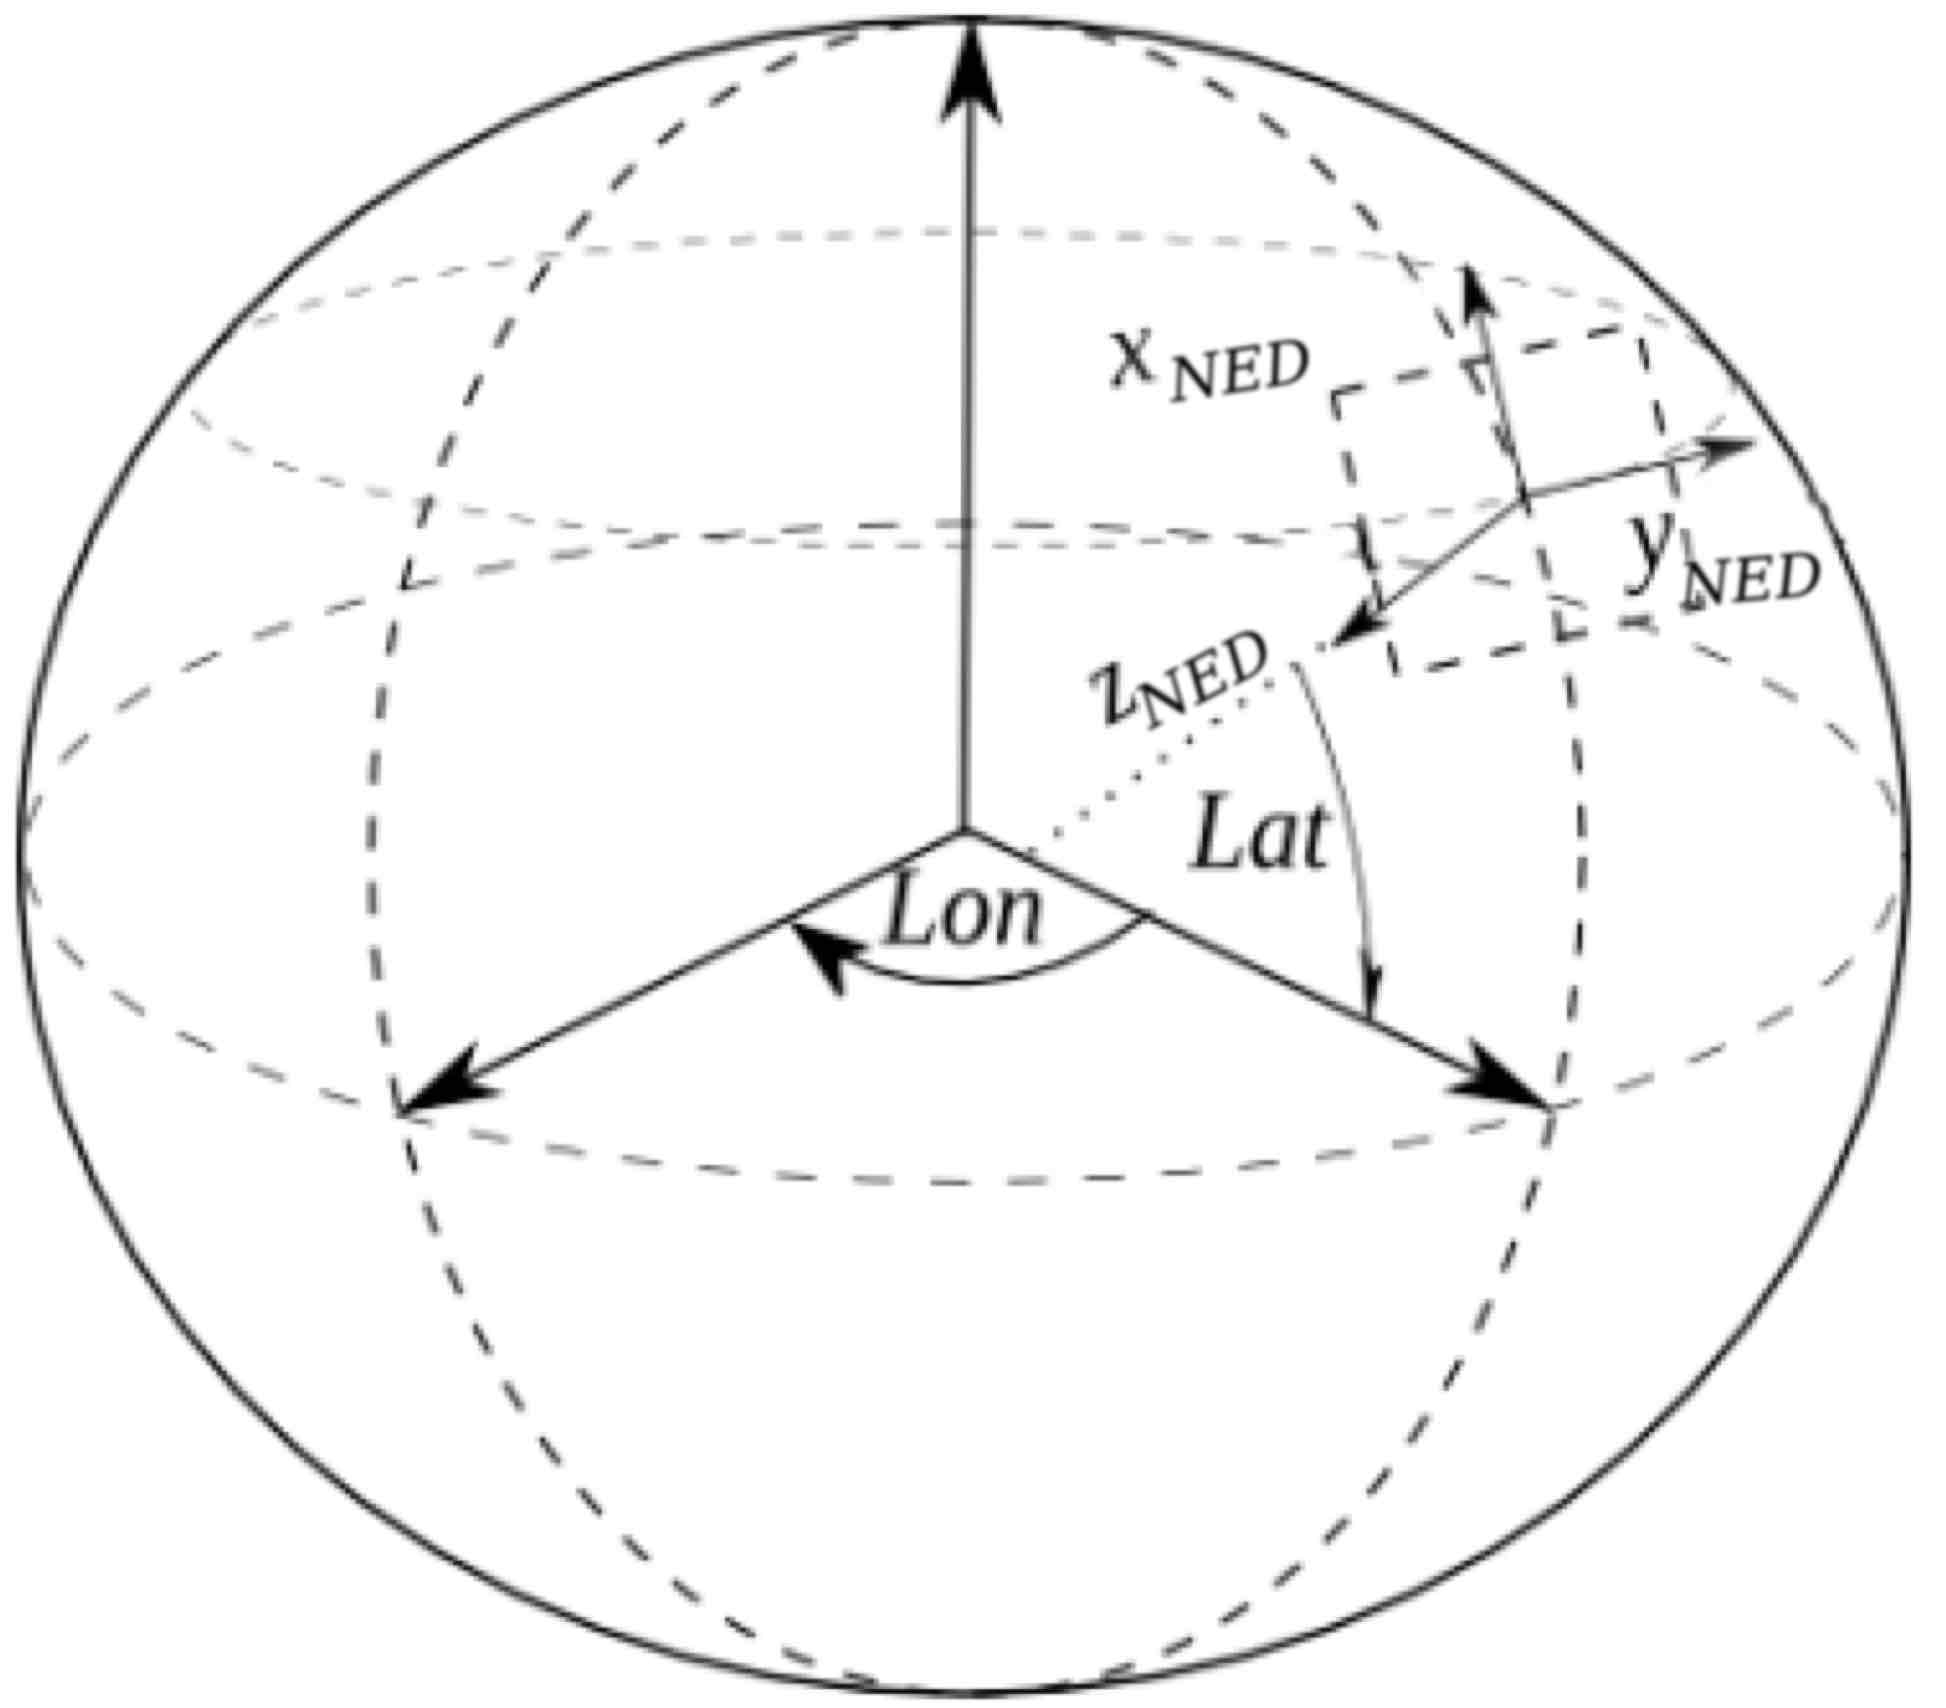
\includegraphics[width=0.4\linewidth]{Immagini/NED.jpg}
    \caption{Sistema di riferimento $NED$ \cite{mscthesis:uav}}
\end{figure}


\subsection{Sistema Assi Corpo FRD}

Il sistema assi corpo, o Front-Right-Down ($FRD$) ha origine nel centro di massa del velivolo. Gli assi sono definiti nel seguente modo:

\begin{sitemize}
    \item Asse ($\hat{x}_{FRD}$) è parallelo alla linea di riferimento della fusoliera ed è diretto nella direzione in cui è rivolto il pilota
    \item Asse ($\hat{y}_{FRD}$) passa attraverso le punte delle ali, con verso positivo verso la destra del velivolo.
    \item Asse ($\hat{z}_{FRD}$) è diretto verso il basso, perpendicolare agli altri due assi.
\end{sitemize}

\begin{figure}[H]
    \centering
    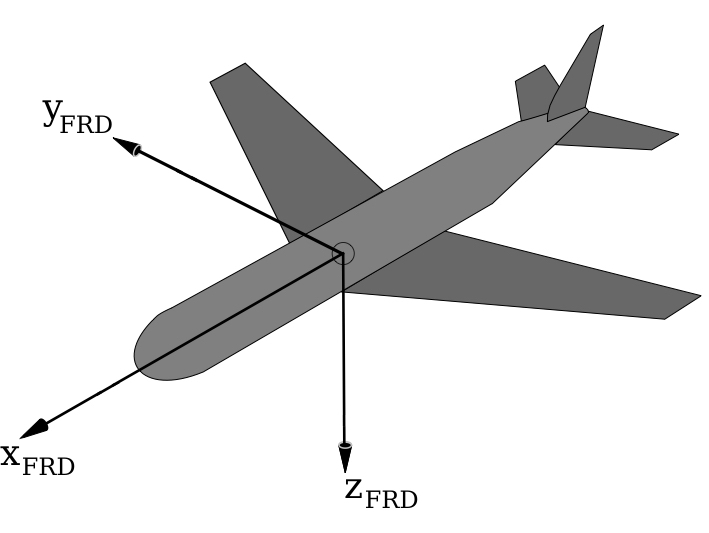
\includegraphics[width=0.42\linewidth]{Immagini/FRD.jpg}
    \caption{Sistema di riferimento $FRD$ \cite{wiki:FRD}}
\end{figure}

\subsection{Sistema Assi di Stabilità}
Solitamente il velivolo presenta un certo angolo di incidenza $\alpha$ rispetto al flusso d'aria durante il volo.
Viene definito quindi il sistema assi di stabilità, i cui versori sono detti $\hat{x}_{S}$, $\hat{y}_{S}$, $\hat{z}_{S}$, ottenuto effettuando una rotazione del sistema di riferimento $FRD$ di un angolo $\alpha$ attorno all'asse $\hat{y}_{FRD}$.

\begin{figure}[H]
    \centering
    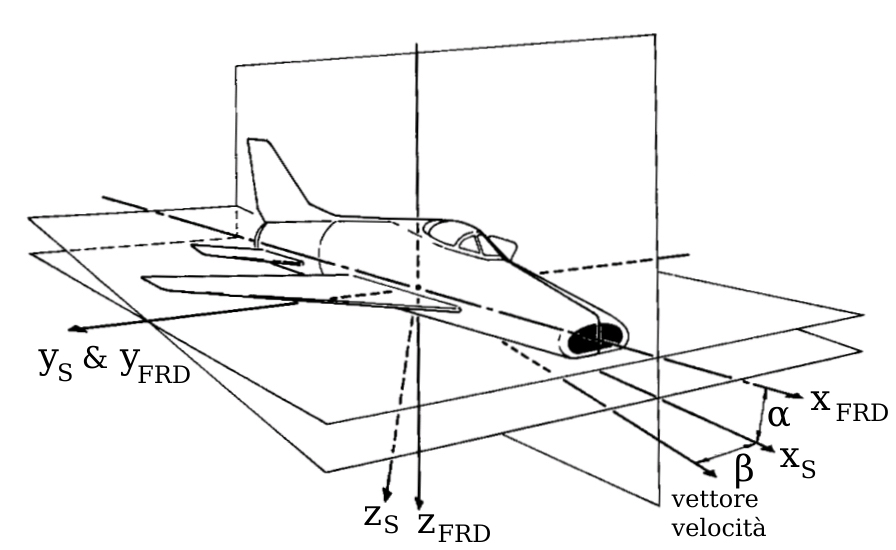
\includegraphics[width=0.5\linewidth]{Immagini/stability.jpg}
    \caption{Sistema di riferimento Assi di Stabilità \cite{mscthesis:jetfighter}}
\end{figure}

\subsection{Sistema Assi Vento}
Un aereo può volare anche con un certo angolo di derapata $\beta$ rispetto al flusso d'aria.
Viene definito quindi il sistema assi vento, i cui versori sono detti $\hat{x}_{W}$, $\hat{y}_{W}$, $\hat{z}_{W}$, ottenuto effettuando una rotazione del sistema assi di stabilità di un angolo $\beta$ attorno all'asse $\hat{z}_{S}$.

\begin{note}
    Si nota che non è necessaria alcuna rotazione attorno all'asse $\hat{x}_{W}$ per allinearlo al vettore velocità, quindi nella trasformazione al sistema assi vento quell'angolo di rotazione rimane 0.
\end{note}

\section{Trasformazioni tra Sistemi di Riferimento}
Poiché le forze e quantità del velivolo saranno descritte in diversi sistemi di riferimento, è necessario convertirle in un unico sistema coerente per poterle utilizzare nelle equazioni del moto.
Di seguito sono descritte le matrici di trasformazione utilizzate nel corso di questa tesi.

\subsubsection{Trasformazione da Sistema NED a FRD}\label{subsec:Eulero}
La trasformazione tra due i sistemi di riferimento avviene attraverso tre rotazioni successive.
I tre angoli, detti angoli di Eulero, si definiscono come segue:
\begin{note}
    Sia $N$ un insieme di punti dato dall'intersezione tra i piani generati dalle coppie di vettori $\hat{x}_{NED}$ $\hat{y}_{NED}$ e $\hat{x}_{FRD}$ $\hat{y}_{FRD}$,
\end{note}
\begin{sitemize}
    \item $\psi$ è l'angolo di imbardata, ovvero l'angolo tra l'insieme di punti $N$ e l'asse $\hat{x}_{FRD}$.
    \item $\theta$ è l'angolo di beccheggio, ovvero l'angolo tra l'asse $\hat{z}_{NED}$ e l'asse $\hat{z}_{FRD}$.
    \item $\phi$ è l'angolo di rollio, ovvero l'angolo tra l'asse $\hat{x}_{NED}$ e l'insieme di punti $N$.
\end{sitemize}

\begin{figure}[H]
    \centering
    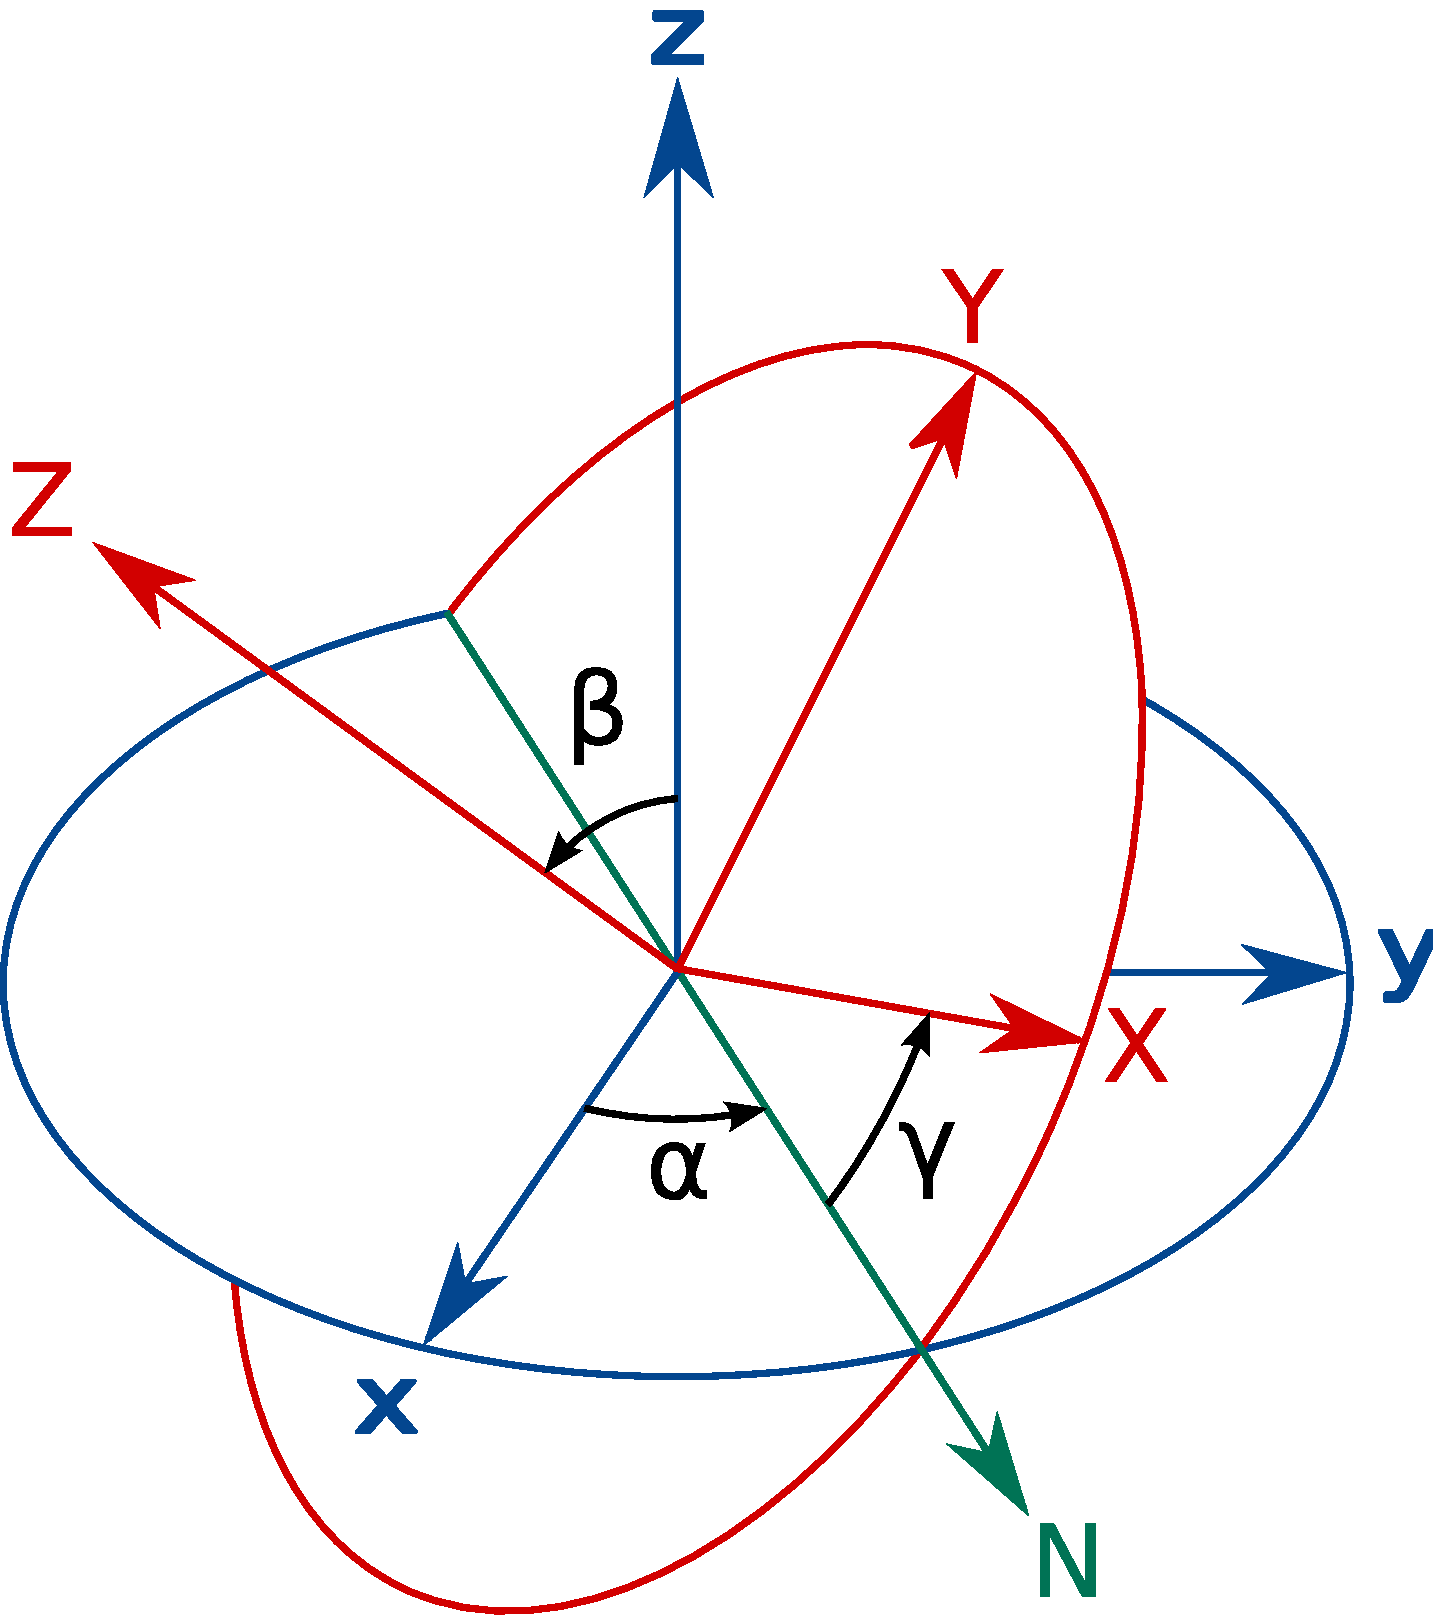
\includegraphics[width=0.35\linewidth]{Immagini/euler_angles.pdf}
    \caption{Trasformazione tra sistemi di riferimento con angoli di Eulero \cite{wiki:eulerangles}}
\end{figure}

La matrice di trasformazione tra i due sistemi di riferimento può essere definita effettuando 3 rotazioni seperate:
\begin{enumerate}
    \setlength{\itemsep}{0pt}
    \setlength{\parskip}{0pt}
    \setlength{\parsep}{0.25em}
    \setlength{\topsep}{0.5em}
    \setlength{\leftmargin}{1em}
    \setlength{\labelwidth}{1em}
    \setlength{\labelsep}{0.5em}
    \item Rotazione di $\psi$ attorno all'asse $\hat{z}_{FRD}$ descritta dalla matrice di rotazione $R_{z}(\psi)$

          Dato un generico punto $\begin{smallmatrix}(x_{NED}&y_{NED})\end{smallmatrix}$ è possibile scomporre le componenti in vettori lungo $\hat{x}_{FRD}$ e $\hat{y}_{FRD}$.
          \begin{figure}[H]
              \centering
              \begin{tikzpicture}[>=stealth, line width=0.4mm]

                  % Psi angle
                  \def\rotation{30}
                  \def\length{4}

                  % Coordinate axes
                  \coordinate (O) at (0,0);
                  \coordinate (xNED) at (0,\length);
                  \coordinate (yNED) at (\length,0);

                  % Rotated coordinates for FRD
                  \coordinate (xFRD) at ({\length*cos(\rotation)},{-\length*sin(\rotation)});
                  \coordinate (yFRD) at ({\length*sin(\rotation)},{\length*cos(\rotation)});

                  % NED frame
                  \draw[->, black] (O) -- (xNED) node[above left] {\textbf{$x_{NED}$}};
                  \draw[->, black] (O) -- (yNED) node[above right] {\textbf{$y_{NED}$}};

                  % FRD frame
                  \draw[->, violet] (O) -- (xFRD) node[below right] {\textbf{$y_{FRD}$}};
                  \draw[->, violet] (O) -- (yFRD) node[right] {\textbf{$x_{FRD}$}};

                  % Dashed projections for x_FRD
                  \draw[->, dashed, blue] ({\length*cos(\rotation)},{-\length*sin(\rotation) + 0.1}) -- (\length,-0.1) node[midway, right, blue] {$y_{NED} \cdot \sin \psi$};
                  \draw[->, dashed, blue] (0, -0.2) -- ({\length*cos(\rotation) - 0.1},{-\length*sin(\rotation) - 0.2}) node[midway, below, rotate=-\rotation, blue] {$y_{NED} \cdot \cos \psi$};

                  % Dashed projections for y_FRD
                  \draw[->, dashed, blue] ({\length*sin(\rotation) - 0.1},{\length*cos(\rotation)}) -- (0.1, \length) node[midway, above, rotate=-{\rotation/2-2}, blue] {$x_{NED} \cdot \sin \psi$};
                  \draw[->, dashed, blue] (0.2, 0) -- ({\length*sin(\rotation) + 0.2},{\length*cos(\rotation) - 0.1}) node[midway, below, rotate={\rotation*2 - 2}, blue] {$x_{NED} \cdot \cos \psi$};

                  % Angles
                  \draw[->] (1.5,0) arc[start angle=0,end angle=-\rotation,radius=1.5] node[midway, right] {$\psi$};

                  \draw[->] (0,1.5) arc[start angle=90,end angle=90-\rotation,radius=1.5]  node[midway, above] {$\psi$};

              \end{tikzpicture}
              \caption{Scomposizione delle componenti}
          \end{figure}


          Sommando poi le componenti proiettate sugli assi $\hat{x}_{FRD}$ e $\hat{y}_{FRD}$ si ottiene:
          \begin{equation*}
              R_{z}(\psi) = \begin{bmatrix}
                  \cos\psi & -\sin\psi & 0 \\
                  \sin\psi & \cos\psi  & 0 \\
                  0        & 0         & 1
              \end{bmatrix}
          \end{equation*}
    \item Rotazione di $\theta$ attorno all'asse $\hat{y}_{FRD}$ descritta dalla matrice di rotazione $R_{y}(\theta)$
          \begin{equation*}
              R_{y}(\theta) = \begin{bmatrix}
                  \cos\theta & 0 & -\sin\theta \\
                  0          & 1 & 0           \\
                  \sin\theta & 0 & \cos\theta
              \end{bmatrix}
          \end{equation*}
    \item Rotazione di $\phi$ attorno all'asse $\hat{x}_{FRD}$ descritta dalla matrice di rotazione $R_{x}(\phi)$
          \begin{equation*}
              R_{x}(\phi) = \begin{bmatrix}
                  1 & 0         & 0        \\
                  0 & \cos\phi  & \sin\phi \\
                  0 & -\sin\phi & \cos\phi \\
              \end{bmatrix}
          \end{equation*}
\end{enumerate}

La matrice di trasformazione completa è quindi data da:
\begin{multline}
    \label{eq:NEDtoFRD}
    C_{NED \rightarrow FRD} = R_{z}(\psi)R_{y}(\theta)R_{x}(\phi) = \\ = \begin{bmatrix}
        \cos\theta\cos\psi                            & \cos\theta\sin\psi                            & -\sin\theta        \\
        \sin\phi\sin\theta\cos\psi - \cos\phi\sin\psi & \sin\phi\sin\theta\sin\psi + \cos\phi\cos\psi & \sin\phi\cos\theta \\
        \cos\phi\sin\theta\cos\psi + \sin\phi\sin\psi & \cos\phi\sin\theta\sin\psi - \sin\phi\cos\psi & \cos\phi\cos\theta
    \end{bmatrix}
\end{multline}

\subsubsection{Trasformazione da Sistema FRD a NED}
Come riportato in \cite{smith_aircraft_flight_mechanics} la matrice di trasformazione $C_{NED \rightarrow FRD}$ è ortogonale, ovvero soddisfa la relazione $C_{NED \rightarrow FRD} \cdot C_{NED \rightarrow FRD}^T = I$.
Di conseguenza, la matrice inversa coincide con la trasposta:
\begin{multline}
    \label{eq:FRDtoNED}
    C_{FRD \rightarrow NED}  = C_{NED \rightarrow FRD}^T = \\
    = \begin{bmatrix}
        \cos\theta\cos\psi & \sin\phi\sin\theta\cos\psi + \cos\phi\sin\psi & \cos\phi\sin\theta\cos\psi - \sin\phi\sin\psi \\
        \cos\theta\sin\psi & \sin\phi\sin\theta\sin\psi - \cos\phi\cos\psi & \cos\phi\sin\theta\sin\psi + \sin\phi\cos\psi \\
        -\sin\theta        & \sin\phi\cos\theta                            & \cos\phi\cos\theta
    \end{bmatrix}
\end{multline}

\subsubsection{Trasformazione da Sistema Assi di Stabilità a FRD}
I due sistemi differiscono per una sola rotazione di un angolo $\alpha$ attorno all'asse $\hat{y}_{S}$. La matrice di trasformazione è definita similmente a quanto fatto per la rotazione di $\theta$ in \eqref{eq:NEDtoFRD}:
\begin{equation}
    \label{eq:StoFRD}
    C_{S \rightarrow FRD} = \begin{bmatrix}
        \cos\alpha & 0 & -\sin\alpha \\
        0          & 1 & 0           \\
        \sin\alpha & 0 & \cos\alpha
    \end{bmatrix}
\end{equation}

\subsubsection{Trasformazione da Sistema Assi Vento a FRD}
I due sistemi differiscono per due rotazioni: una di $\beta$ attorno all'asse $\hat{z}_{S}$ e una di $\alpha$ attorno all'asse $\hat{y}_{FRD}$. La matrice di rotazione è definita nel seguente modo, similmente a quanto fatto per la rotazione di $\psi$ in \eqref{eq:NEDtoFRD}:
\begin{equation}
    \label{eq:WtoFRD}
    \begin{split}
        C_{W \rightarrow FRD} & = \begin{bmatrix}
                                      \cos\alpha & 0 & -\sin\alpha \\
                                      0          & 1 & 0           \\
                                      \sin\alpha & 0 & \cos\alpha
                                  \end{bmatrix} \cdot \begin{bmatrix}
                                                          \cos\beta & -\sin\beta & 0 \\
                                                          \sin\beta & \cos\beta  & 0 \\
                                                          0         & 0          & 1
                                                      \end{bmatrix} \\ &= \begin{bmatrix}
            \cos\alpha\cos\beta & -\cos\alpha\sin\beta & -\sin\alpha \\
            \sin\beta           & \cos\beta            & 0           \\
            \sin\alpha\cos\beta & -\sin\alpha\sin\beta & \cos\alpha
        \end{bmatrix}
    \end{split}
\end{equation}

\section{Superfici di Controllo}
Le superfici di controllo sono dei dispositivi in grado di modificare l'assetto del velivolo. Sono controllate dal pilota o dall'autopilota.

\begin{itemize}
    \item \textbf{Alettoni}: sono posizionate all'estremità delle ali. Operano in modalità differenziale: quando uno si alza, l'altro si abbassa.
          Il loro movimento influenza l'angolo di rollio $\phi$ dell'aeromobile.
          Sono controllati ruotando la cloche e la loro deflessione è indicata con $\delta_a (t)$;
    \item \textbf{Equilibratore}: è la parte mobile del piano orizzontale di coda di un aeromobile. I due lati si muovono all'unisono.
          Il suo movimento influenza l'angolo di beccheggio $\theta$ dell'aeromobile.
          È controllato mediante la traslazione avanti e indietro della cloche e la sua deflessione è indicata con $\delta_e (t)$;

    \item \textbf{Timone}: è una superficie di controllo montata al piano verticale di coda.
          Il suo movimento influenza l'angolo di imbardata $\psi$ dell'aeromobile.
          È controllato attraverso i pedali e la sua deflessione è indicata con $\delta_r (t)$;
\end{itemize}

\begin{figure}[H]
    \centering
    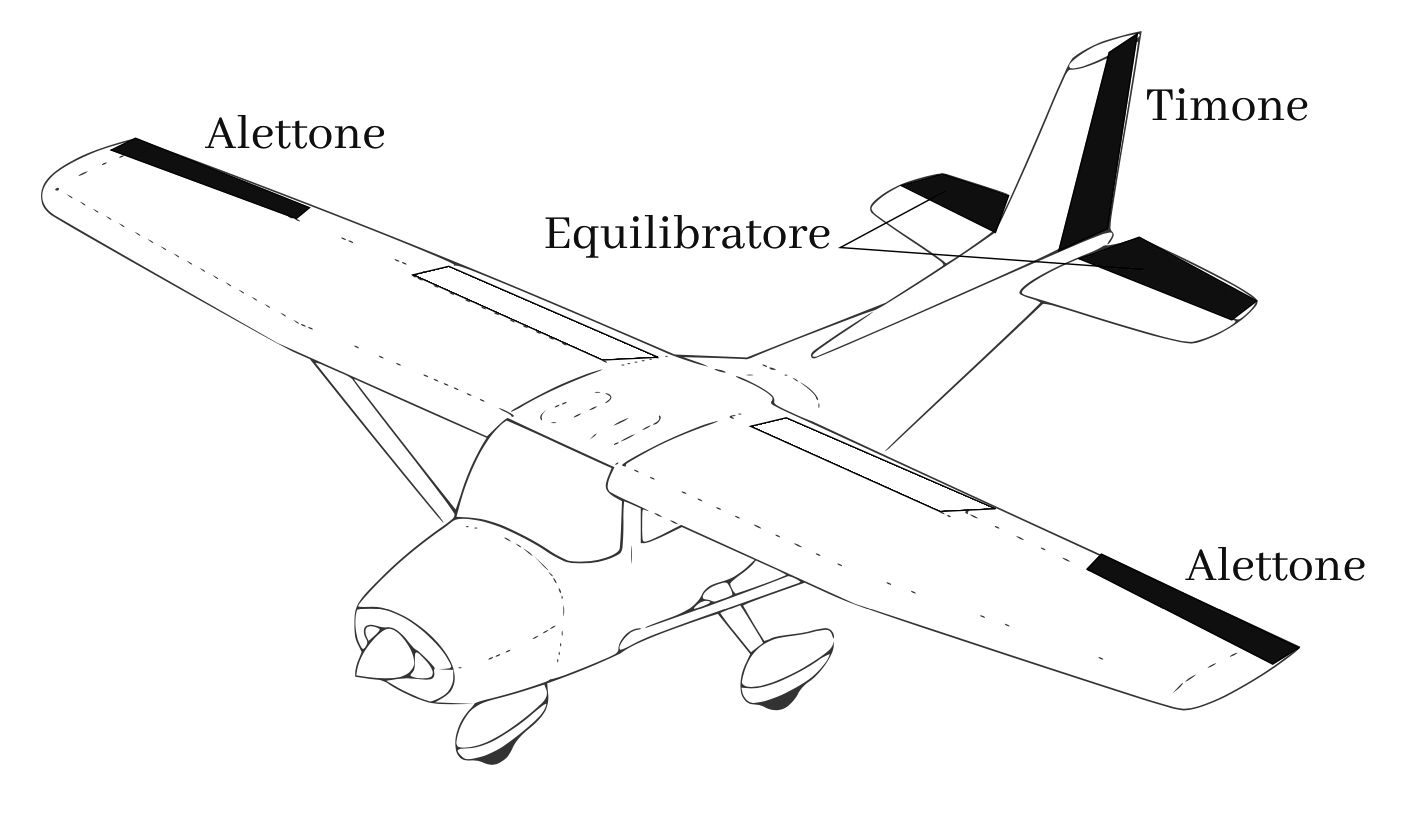
\includegraphics[width=0.55\linewidth]{Immagini/ControlSurfaces.jpg}
    \caption{Superfici di Controllo \cite{smith_aircraft_flight_mechanics}}
\end{figure}

\chapter{Modellizzazione}
\section{Variabili del sistema}

\subsection{Forze}
\subsubsection{Forza Peso}
La forza peso è ben definita nel sistema di riferimento $NED$, in quanto è allineata con l'asse $\hat{z}_{NED}$. Può essere trasformata nel sistema di riferimento $FRD$ tramite la matrice di rotazione definita in \eqref{eq:NEDtoFRD}:
\begin{equation}
    \label{eq:Fpeso}
    \left(\vec{F}_P(t)\right)_{FRD} = C_{NED \rightarrow FRD}\begin{bmatrix}
        0 \\
        0 \\
        mg
    \end{bmatrix}_{NED} = \begin{bmatrix}
        -mg\sin\theta (t)          \\
        mg\sin\phi(t)\cos\theta(t) \\
        mg\cos\phi(t)\cos\theta(t)
    \end{bmatrix}_{FRD}
\end{equation}

\begin{note}
    Nella formula $m$ e $g$ sono delle costanti che rappresentano rispettivamente la massa del velivolo e l'accelerazione di gravità.
\end{note}

\subsubsection{Forza Propulsiva}
La forza propulsiva è definita nel sistema di riferimento FRD, in generale non è allineata all'asse $\hat{x}_{FRD}$, ma può essere scomposta in due componenti:

\begin{equation}
    \label{eq:Fpropulsiva}
    \left(\vec{F}_T(t)\right)_{FRD} = \begin{bmatrix}
        T(t) \cos\epsilon \\
        0                 \\
        -T(t) \sin\epsilon
    \end{bmatrix}_{FRD}
\end{equation}

\begin{figure}[H]
    \centering
    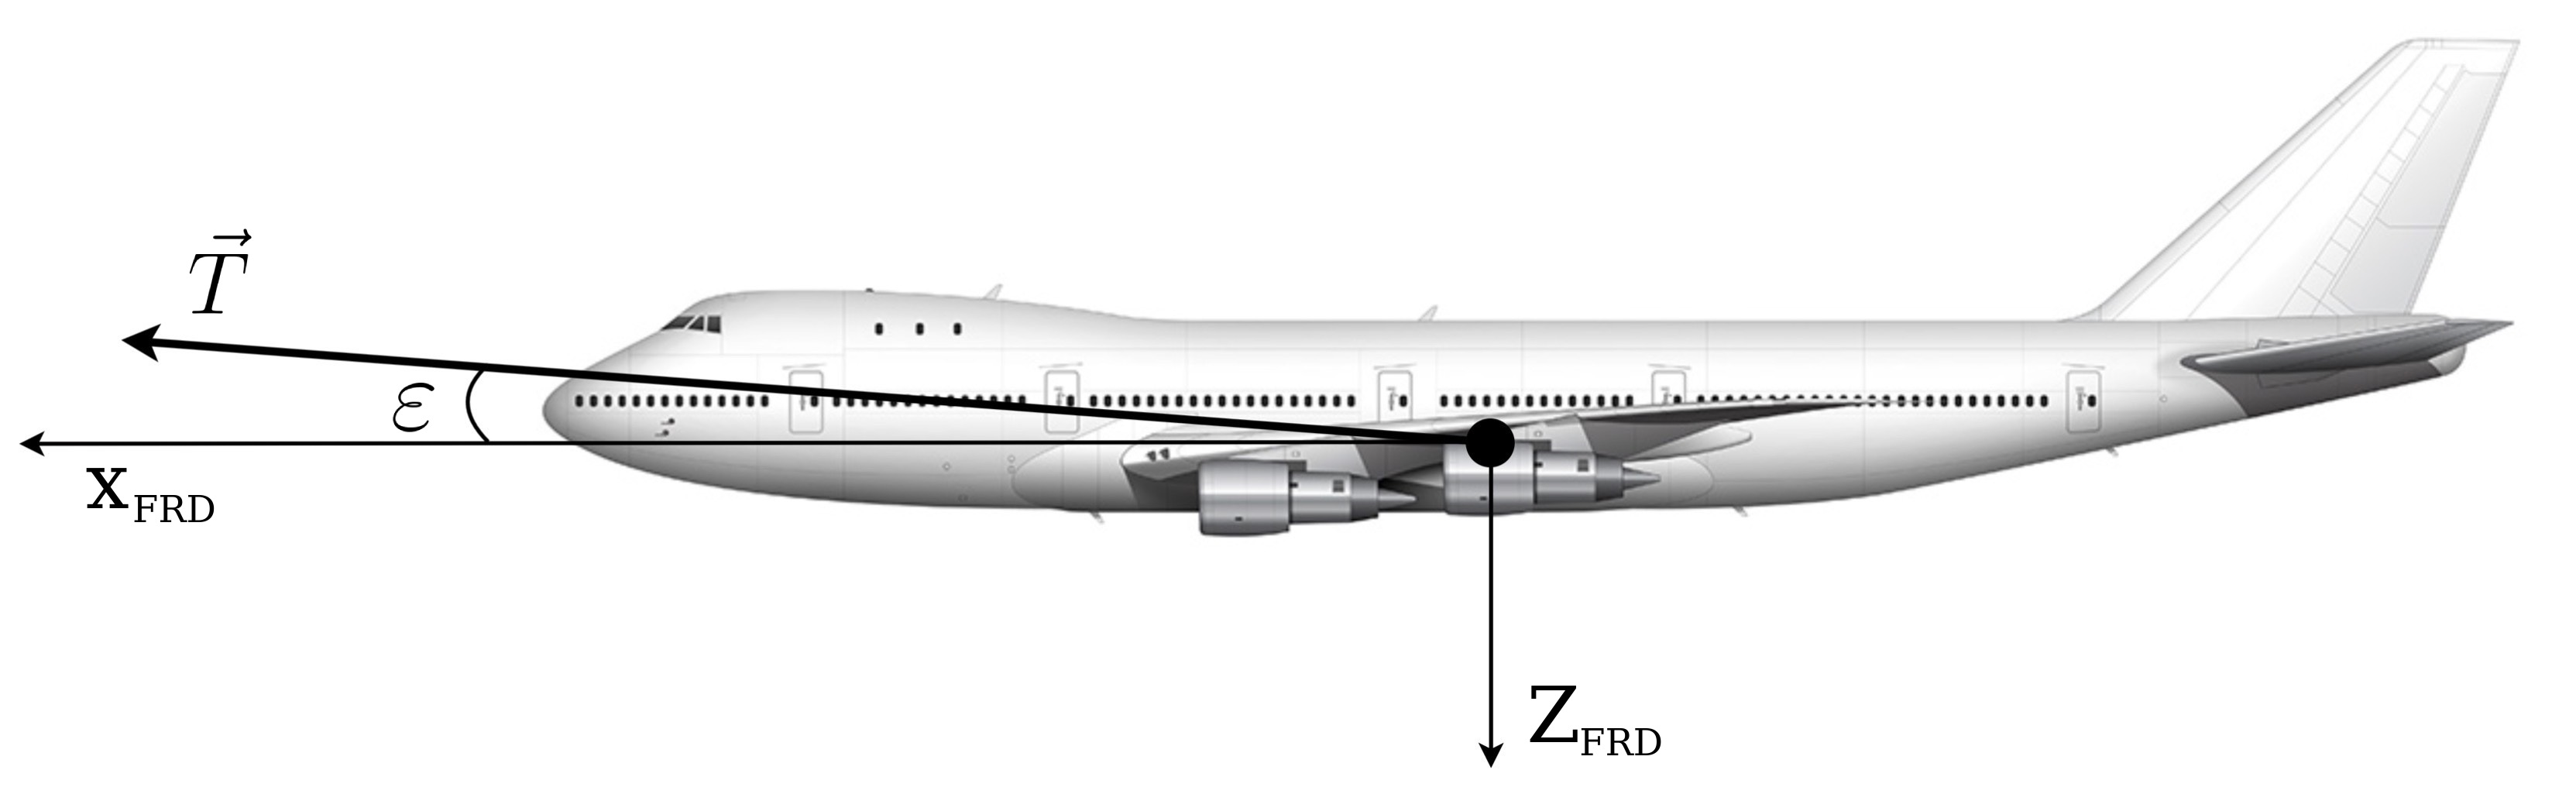
\includegraphics[width=0.7\linewidth]{Immagini/forza_propulsiva.jpg}
    \caption{Vettore $\vec{T}(t)$ e il suo angolo $\epsilon$}
\end{figure}

\begin{note}
    Nella formula $\epsilon$ è una costante determinata dalla struttura del velivolo che rappresenta l'angolo tra il vettore $\vec{T}$ e l'asse $\hat{x}_{FRD}$
\end{note}

\subsubsection{Forze Aerodinamiche}
Le forze aerodinamiche sono ben definite nel sistema di riferimento assi di stabilità.
\begin{equation*}
    \left(\vec{F}_A(t)\right)_{S} = \begin{bmatrix}
        -F_{A_x}(t) \\
        F_{A_y}(t)  \\
        -F_{A_z}(t)
    \end{bmatrix}_{S}
\end{equation*}

In questo caso $F_{A_z}(t)$ rappresenta la portanza, normale al flusso d'aria, mentre $F_{A_x}(t)$ la resistenza aerodinamica, opposta al flusso d'aria.

$F_{A_y}(t)$ è la componente laterale della forza, dovuta all'angolo di derapata $\beta(t)$.

Si possono esprimere le forze aerodinamiche nel sistema di riferimento $FRD$ tramite la matrice di rotazione definita in \eqref{eq:StoFRD}:
\begin{equation}
    \label{eq:Faerodinamica}
    \left(\vec{F}_A(t)\right)_{FRD} = C_{S \rightarrow FRD}\left(\vec{F}_A(t)\right)_{S} = \begin{bmatrix}
        -F_{A_x}(t) \cos\alpha(t) + F_{A_z}(t) \sin\alpha(t) \\
        F_{A_y}(t)                                           \\
        -F_{A_x}(t)\sin\alpha(t) - F_{A_z}(t)\cos\alpha(t)
    \end{bmatrix}_{FRD}
\end{equation}

\begin{note}
    $F_{A_x}(t), F_{A_y}(t), F_{A_z}(t)$ sono funzioni non lineari di altre variabili del sistema. Questa dipendenza verrà analizzata in maggior dettaglio nella sezione \ref{sec:derivateStabilita}.
\end{note}
\subsection{Velocità Angolare}

Diremo $\vec{w}_{FRD}$ la velocità angolare del sistema di riferimento $FRD$ rispetto al sistema inerziale $NED$.

Il sistema $FRD$ è stato definito a partire dal sistema $NED$ come una serie di tre rotazioni i cui angoli sono detti angoli di Eulero \ref{subsec:Eulero}.
Tuttavia la loro derivata non fornisce $\vec{w}_{FRD}$ in quanto i tre angoli non sono descritti nello stesso sistema di riferimento è quindi necessario applicare delle rotazioni:

\begin{equation}
    \label{eq:EulerotoVelocitaAngolare}
    \begin{split}
        \vec{w}_{FRD}(t) & = \begin{bmatrix}
                                 p(t) \\
                                 q(t) \\
                                 r(t)
                             \end{bmatrix} = R_{x}(\phi)R_{y}(\theta) \begin{bmatrix}
                                                                          0 \\
                                                                          0 \\
                                                                          \dot{\psi}(t)
                                                                      \end{bmatrix} + R_{x}(\phi) \begin{bmatrix}
                                                                                                      0               \\
                                                                                                      \dot{\theta}(t) \\
                                                                                                      0
                                                                                                  \end{bmatrix} + I_3 \begin{bmatrix}
                                                                                                                          \dot{\phi}(t) \\
                                                                                                                          0             \\
                                                                                                                          0
                                                                                                                      \end{bmatrix} =
        \\ & = \begin{bmatrix}
            1 & 0            & -\sin\theta(t)           \\
            0 & \cos\phi(t)  & \sin\phi(t)\cos\theta(t) \\
            0 & -\sin\phi(t) & \cos\phi(t)\cos\theta(t)
        \end{bmatrix}\begin{bmatrix}
            \dot{\phi}(t)   \\
            \dot{\theta}(t) \\
            \dot{\psi}(t)
        \end{bmatrix}
    \end{split}
\end{equation}

\subsection{Velocità}
La velocità del velivolo è la velocità del sistema di riferimento $FRD$ rispetto al sistema inerziale $NED$.

\begin{equation}
    \label{eq:velocitaFRD}
    \vec{V}_{FRD}(t) = \begin{bmatrix}
        u(t) \\
        v(t) \\
        w(t)
    \end{bmatrix}_{FRD}
\end{equation}

\subsubsection{Velocità nel Sistema Assi Vento}
Una rappresentazione più naturale del vettore velocità è nel sistema di riferimento assi vento, in quanto è parallelo a $\hat{x}_{W}$.
È poi possibile cambiare il sistema di riferimento ottenendo così una rappresentazione polare della velocità nel sistema $FRD$:

\begin{equation}
    \label{eq:velocitaWind}
    \vec{V}_{FRD}(t) = \begin{bmatrix}
        u(t) \\
        v(t) \\
        w(t)
    \end{bmatrix}_{FRD} = C_{W \rightarrow FRD}\begin{bmatrix}
        |\vec{V}_{FRD}(t)| \\
        0                  \\
        0
    \end{bmatrix}_{W} = |\vec{V}_{FRD}(t)|\begin{bmatrix}
        \cos\alpha(t)\cos\beta(t) \\
        \sin\beta(t)              \\
        \sin\alpha(t)\cos\beta(t)
    \end{bmatrix}
\end{equation}

\begin{figure}[H]
    \centering
    \includegraphics[width=0.4\linewidth]{Immagini/velocità_assi_vento.jpg}
    \caption{Vettore $\vec{V}_{FRD}$ e i suoi angoli $\alpha(t)$ e $\beta(t)$}
\end{figure}

\subsubsection{Velocità nel Sistema NED}
Un'altra rappresentazione utile della velocità è nel sistema di riferimento $NED$, dove può essere espressa come:
\begin{multline}
    \label{eq:velocitaNED}
    \vec{V}_{NED}(t) = \begin{bmatrix}
        \dot{x}(t) \\
        \dot{y}(t) \\
        \dot{z}(t)
    \end{bmatrix}_{NED} = C_{FRD \rightarrow NED}\begin{bmatrix}
        u(t) \\
        v(t) \\
        w(t)
    \end{bmatrix}_{FRD} = \\ = \begin{bmatrix}
        \cos\theta\cos\psi \: u + \left(\sin\phi\sin\theta\cos\psi + \cos\phi\sin\psi\right)v + \left(\cos\phi\sin\theta\cos\psi - \sin\phi\sin\psi\right)w \\
        \cos\theta\sin\psi \: u + \left(\sin\phi\sin\theta\sin\psi - \cos\phi\cos\psi\right)v + \left(\cos\phi\sin\theta\sin\psi + \sin\phi\cos\psi\right)w \\
        -\sin\theta \: u + \sin\phi\cos\theta \: v + \cos\phi\cos\theta \: w
    \end{bmatrix}
\end{multline}

\textbf{Nota:} \textit{Per semplicità di lettura è omessa la dipendenza dal tempo di $\theta$, $\phi$, $\psi$, $u$, $v$, $w$}

\subsection{Accelerazione}

Affinché siano valide le equazioni cardinali è necessario applicarle su un sistema di riferimento inerziale, per questo motivo è necessario calcolare $\vec{a}_{NED}$.
Per farlo si sfrutta la relazione di Poisson, $\frac{d}{dt}\vec{u}(t) = \vec{w}_{FRD}(t) \times \vec{u}(t)$, la cui dimostrazione è illustrata in \cite{zotto_fisica1}

\begin{figure}[H]
    \centering
    \begin{tikzpicture}
        \draw[->] (-3,0)--(3,0) node[right]{$x$};
        \draw[->] (0,-1)--(0,3) node[above]{$y$};
        \draw[line width=2pt,blue,-stealth](0,2)--(-0.65,2) node[left]{$\frac{d}{dt}\vec{u}(t)$};
        \draw[line width=2pt,-stealth](0,0)--(0, 2) node[right]{$\vec{u}(t)$};
        \draw[thick,orange] (0,0) circle (0.25);
        \fill[orange] (0,0) circle (2pt);
        \node[orange, anchor=south west] at (0.22, 0.22) {$\vec{w}_{FRD}(t)$};
        \draw[thick,->, orange] (0,1) arc[start angle=90,end angle=120,radius=1.2];
    \end{tikzpicture}
    \caption{Intuizione grafica alla relazione di Poisson}
\end{figure}

\begin{equation}
    \label{eq:accelerazioneNED}
    \begin{split}
        \vec{a}_{NED}(t) & = \left(\frac{d}{d t}\vec{V}_{FRD}(t)\right)_{NED} = \sum_{i=x,y,z} \frac{d}{d t}\left(V_i(t)\vec{u}_i(t)\right) = \\
                         & = \sum_{i=x,y,z} a_i(t)\vec{u}_i(t) + V_i(t)\left(\vec{w}_{FRD}(t)\times\vec{u}_i(t)\right) =                      \\
                         & = \left(\frac{d}{d t} \vec{V}_{FRD}(t)\right)_{FRD} + \vec{w}_{FRD}(t)\times\vec{V}_{FRD}(t) =                     \\
                         & = \begin{bmatrix}
                                 \dot{u}(t) \\
                                 \dot{v}(t) \\
                                 \dot{w}(t)
                             \end{bmatrix} + \begin{bmatrix}
                                                 p(t) \\
                                                 q(t) \\
                                                 r(t)
                                             \end{bmatrix}\times \begin{bmatrix}
                                                                     u(t) \\
                                                                     v(t) \\
                                                                     w(t)
                                                                 \end{bmatrix}
        = \begin{bmatrix}
              \dot{u} + \left(qw - rv\right) \\
              \dot{v} + \left(ru - pw\right) \\
              \dot{w} + \left(pv - qu\right)
          \end{bmatrix}
    \end{split}
\end{equation}

\textbf{Nota:} \textit{Per semplicità di lettura è omessa la dipendenza dal tempo di u, v, w, p, q, r (e derivate).}

\subsection{Momento Angolare}
Il momento angolare di una massa infinitesimale $dm$ appartenente al velivolo è definito come:
\begin{equation*}
    d\vec{H}_{dm}(t) = \vec{r}_{dm}\times \left(\vec{V}_{dm}(t)\right)_{NED} dm
\end{equation*}

Dove $\vec{r}_{dm}$ è la posizione della massa $dm$ rispetto al centro di massa dell'aereomobile.

\begin{figure}[H]
    \centering
    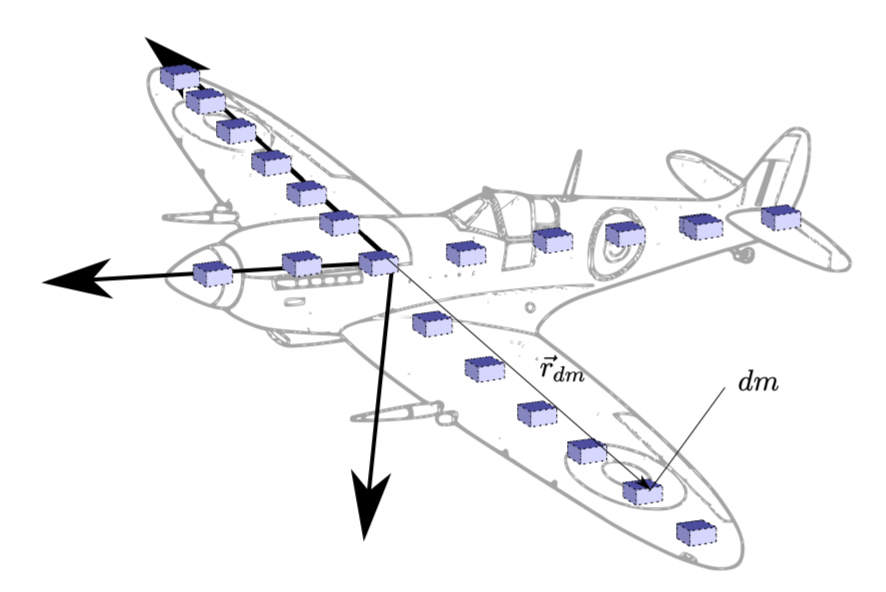
\includegraphics[width=0.5\linewidth]{Immagini/momento_angolare.jpg}
    \caption{Aeromobile descritto da masse infinitesimali \cite{smith_aircraft_flight_mechanics}}
\end{figure}

\subsubsection{Velocità Assoluta}
La velocità assoluta, nel sistema di riferimento inerziale viene calcolata in modo simile a quanto fatto per l'accelerazione:

\begin{equation*}
    \begin{split}
        \left(\vec{V}_{dm}(t)\right)_{NED} & = \left(\frac{d}{d t}\vec{r}_{dm}\right)_{NED} = \left(\frac{d}{d t}\vec{r}_{dm}\right)_{FRD} + \vec{w}_{FRD}(t) \times \vec{r}_{dm} = \\ &= \vec{w}_{FRD}(t) \times \vec{r}_{dm} = \begin{bmatrix}
            q(t)z_{dm} - r(t)y_{dm} \\
            r(t)x_{dm} - p(t)z_{dm} \\
            p(t)y_{dm} - q(t)x_{dm}
        \end{bmatrix}
    \end{split}
\end{equation*}

\begin{note}
    Qui si assume che $\vec{r}_{dm}$ sia costante nel tempo, si sta quindi assumendo che il velivolo sia un corpo rigido, ovvero con flessioni della struttura trascurabili.
\end{note}

\subsubsection{Momento Angolare Infinitesimo}
Il momento angolare di una massa infinitesimale $dm$ è quindi:

\begin{equation*}
    d\vec{H}_{dm}(t) = \vec{r}_{dm}\times \left(\vec{V}_{dm}(t)\right)_{NED} dm = \begin{bmatrix}
        p(t)\left(y_{dm}^2 + z_{dm}^2\right) - q(t)\:x_{dm}y_{dm} - r(t)\:x_{dm}z_{dm} \\
        q(t)\left(x_{dm}^2 + z_{dm}^2\right) - r(t)\:y_{dm}z_{dm} - p(t)\:x_{dm}y_{dm} \\
        r(t)\left(x_{dm}^2 + y_{dm}^2\right) - p(t)\:x_{dm}z_{dm} - q(t)\:y_{dm}z_{dm}
    \end{bmatrix} dm
\end{equation*}

\subsubsection{Momento Angolare Totale}
Il momento angolare totale è l'integrale del momento angolare infinitesimo sul volume dell'aeromobile:

\begin{align*}
    \vec{H}(t) & = \int_{V} d\vec{H}_{dm}(t) dm = \\ &= \begin{bmatrix}
        p(t)\int_V\left(y_{dm}^2 + z_{dm}^2\right) dm - q(t)\int_Vx_{dm}y_{dm}dm - r(t)\int_Vx_{dm}z_{dm}dm \\
        q(t)\int_V\left(x_{dm}^2 + z_{dm}^2\right) dm - r(t)\int_Vy_{dm}z_{dm}dm - p(t)\int_Vx_{dm}y_{dm}dm \\
        r(t)\int_V\left(x_{dm}^2 + y_{dm}^2\right) dm - p(t)\int_Vx_{dm}z_{dm}dm - q(t)\int_Vy_{dm}z_{dm}dm
    \end{bmatrix}
\end{align*}

Gli integrali così ottenuti sono definiti come i momenti e i prodotti di inerzia del velivolo \cite{smith_aircraft_flight_mechanics}:
\begin{equation*}
    \begin{split}
        I_{xx} = \int_V \left(y_{dm}^2 + z_{dm}^2\right) dm \\
        I_{yy} = \int_V \left(x_{dm}^2 + z_{dm}^2\right) dm \\
        I_{zz} = \int_V \left(x_{dm}^2 + y_{dm}^2\right) dm \\
        I_{xy} = I_{yx} = \int_V x_{dm}y_{dm} dm            \\
        I_{xz} = I_{zx} = \int_V x_{dm}z_{dm} dm            \\
        I_{yz} = I_{yz} = \int_V y_{dm}z_{dm} dm
    \end{split}
\end{equation*}

Sostituendo questi integrali nella definizione di $\vec{H}$ si ottiene:

\begin{equation*}
    \vec{H}(t) = \begin{bmatrix}
        I_{xx}p(t) - I_{xy}q(t) - I_{xz}r(t) \\
        I_{yy}q(t) - I_{yz}r(t) - I_{xy}p(t) \\
        I_{zz}r(t) - I_{xz}p(t) - I_{yz}q(t)
    \end{bmatrix} = \begin{bmatrix}
        I_{xx}   & - I_{xy} & - I_{xz} \\
        - I_{yx} & I_{yy}   & - I_{yz} \\
        - I_{xz} & - I_{zy} & I_{zz}
    \end{bmatrix} \vec{w}_{FRD}(t) = I \vec{w}_{FRD}(t)
\end{equation*}

\begin{note}
    $I$ è definito come il \textbf{tensore di inerzia}.
\end{note}

Nel caso del Boeing 747 il velivolo è simmetrico lungo il suo asse longitudinale, quindi $I_{xy}=I_{yx}=I_{yz}=I_{zy}=0$:
\begin{equation}
    \label{eq:TensoreInerzia}
    I = \begin{bmatrix}
        I_{xx}   & 0      & - I_{xz} \\
        0        & I_{yy} & 0        \\
        - I_{zx} & 0      & I_{zz}
    \end{bmatrix}
\end{equation}

\subsubsection{Momento Angolare}
Il momento angolare è quindi definito come:
\begin{equation}
    \label{eq:momentoAngolare}
    \vec{H}(t) = I \vec{w}_{FRD}(t) = \begin{bmatrix}
        I_{xx}p(t) - I_{xz}r(t) \\
        I_{yy}q(t)              \\
        - I_{xz}p(t) + I_{zz}r(t)
    \end{bmatrix}
\end{equation}

\section{Equazioni del Moto}

\subsection{Prima Equazione Cardinale}
La prima equazione cardinale del moto è definita come:

\begin{equation*}
    \vec{F}_P(t) + \vec{F}_T(t) + \vec{F}_A = m\left(\frac{d}{dt}\vec{V}_{FRD}(t)\right)_{NED} = m\cdot\vec{a}_{NED}(t)
\end{equation*}

Sostituendo quanto trovato in \eqref{eq:Fpeso}, \eqref{eq:Fpropulsiva}, \eqref{eq:Faerodinamica} e \eqref{eq:accelerazioneNED} si ottiene:

\begin{multline}
    \label{eq:primaEquazioneCardinale}
    m\begin{bmatrix}
        \dot{u}(t) + \left(q(t)w(t) - r(t)v(t)\right) \\
        \dot{v}(t) + \left(r(t)u(t) - p(t)w(t)\right) \\
        \dot{w}(t) + \left(p(t)v(t) - q(t)u(t)\right)
    \end{bmatrix} = \\
    = mg\begin{bmatrix}
        -\sin\theta(t)           \\
        \sin\phi(t)\cos\theta(t) \\
        \cos\phi(t)\cos\theta(t)
    \end{bmatrix} + \begin{bmatrix}
        T(t) \cos\epsilon \\
        0                 \\
        -T(t) \sin\epsilon
    \end{bmatrix} + \begin{bmatrix}
        -F_{A_x}(t) \cos\alpha(t) + F_{A_z}(t) \sin\alpha(t) \\
        F_{A_y}(t)                                           \\
        -F_{A_x}(t)\sin\alpha(t) - F_{A_z}(t)\cos\alpha(t)
    \end{bmatrix}
\end{multline}

\subsection{Seconda Equazione Cardinale}
La seconda equazione cardinale del moto è definita come:

\begin{equation*}
    \vec{M}(t) = \left(\frac{d}{dt}\vec{H}(t)\right)_{NED}
\end{equation*}

Sostituendo quanto trovato in \eqref{eq:momentoAngolare} e \eqref{eq:EulerotoVelocitaAngolare}, e applicando la relazione di Poisson si ottiene:

\begin{equation*}
    \begin{split}
        \vec{M}(t) = \begin{bmatrix}
                         L(t) \\
                         M(t) \\
                         N(t)
                     \end{bmatrix} & = \left(\frac{d}{dt} \vec{H}(t)\right)_{NED} = \left(\frac{d}{d t} \vec{H}(t)\right)_{FRD} + \vec{w}_{FRD}(t)\times\vec{H}(t)
        \\ & = I\left(\frac{d}{d t} \vec{w}_{FRD}(t)\right)_{FRD} + \vec{w}_{FRD}(t)\times \left(I\vec{w}_{FRD}(t)\right)
        \\ & = \begin{bmatrix}
            I_{xx}\dot{p} - I_{xz}\dot{r} \\
            I_{yy}\dot{q}                 \\
            - I_{xz}\dot{p} + I_{zz}\dot{r}
        \end{bmatrix} + \begin{bmatrix}
            q\left(- I_{xz}p + I_{zz}r\right) - r\left(I_{yy}q\right)           \\
            r\left(I_{xx}p - I_{xz}r\right) - p\left(- I_{xz}p + I_{zz}r\right) \\
            p\left(I_{yy}q\right) - q\left(I_{xx}p - I_{xz}r\right)
        \end{bmatrix}
    \end{split}
\end{equation*}

Complessivamente si ottiene:
\begin{equation}
    \label{eq:secondaEquazioneCardinale}
    \begin{bmatrix}
        L \\
        M \\
        N
    \end{bmatrix} = \begin{bmatrix}
        \dot{p}I_{xx} + qr\left(I_{zz} - I_{yy}\right) - \left(\dot{r} + pq\right)I_{xz} \\
        \dot{q}I_{yy} + pr\left(I_{xx} - I_{zz}\right) + \left(p^2 - r^2\right)I_{xz}    \\
        \dot{r}I_{zz} + pq\left(I_{yy} - I_{xx}\right) + \left(qr - \dot{p}\right)I_{xz}
    \end{bmatrix}
\end{equation}

\textbf{Nota:} \textit{Per semplicità di lettura, sono omesse le dipendenze da altre variabili di L, M, N, p, q, r (e derivate).}

\subsection{Segnali e Costanti del Sistema}

\renewcommand{\arraystretch}{1.2}
\begin{table}[H]
    \begin{tabularx}{\textwidth}{|c|X|}
        \hline
        \multicolumn{2}{|l|}{\textbf{Costanti}}                                                                                                                                    \\
        \hline
        $m$                                    & Massa del velivolo                                                                                                                \\
        $g$                                    & Accelerazione di gravità                                                                                                          \\
        $\epsilon$                             & Angolo tra il vettore $\vec{T}$ e l'asse $\hat{x}_{FRD}$                                                                          \\
        $I_{xx}$, $I_{yy}$, $I_{zz}$, $I_{xz}$ & Componenti del tensore di inerzia                                                                                                 \\
        \hline
        \multicolumn{2}{|l|}{\textbf{Segnali}}                                                                                                                                     \\
        \hline
        $u$, $v$, $w$                          & Componenti del vettore $\vec{V}_{FRD}$ che rappresenta la velocità del sistema $FRD$ rispetto al sistema inerziale $NED$          \\
        $p$, $q$, $r$                          & Componenti del vettore $\vec{w}_{FRD}$ che rappresenta la velocità angolare del sistema $FRD$ rispetto al sistema inerziale $NED$ \\
        $\phi$                                 & Angolo di rollio                                                                                                                  \\
        $\psi$                                 & Angolo di imbardata                                                                                                               \\
        $\theta$                               & Angolo di beccheggio                                                                                                              \\
        $L$, $M$, $N$                          & Componenti del momento meccanico                                                                                                  \\
        $T$                                    & Modulo della forza propulsiva                                                                                                     \\
        $F_{A_x}$, $F_{A_y}$, $F_{A_z}$        & Componenti delle forze aerodinamiche                                                                                              \\
        \hline
    \end{tabularx}
\end{table}

I 16 segnali e le 7 costanti sono legati da 9 equazioni (descritte in \eqref{eq:secondaEquazioneCardinale}, \eqref{eq:primaEquazioneCardinale}, \eqref{eq:EulerotoVelocitaAngolare}), che descrivono posizione e assetto del velivolo nello spazio.
\section{Linearizzazione}
Le equazioni ottenute in \eqref{eq:primaEquazioneCardinale} e \eqref{eq:secondaEquazioneCardinale} non sono lineari e non possono essere risolte analiticamente.
Per questo motivo è utile determinare un modello lineare che approssimi il comportamento del sistema attorno ad un certo punto, nel nostro caso il volo rettilineo simmetrico uniforme.

Per fare questo vengono risolte le equazioni del moto in un punto di equilibrio (indicheremo tali soluzioni con $\bar{x}$), così da poter riscrivere le variabili di stato come piccole perturbazioni rispetto a tale punto (che indicheremo con $\widetilde{x}(t)$), come descritto in \cite{zampieri_dispensa_controlli}.

\begin{equation*}
    x(t) = \bar{x} + \tilde{x}(t)
\end{equation*}

\subsection{Punto di Equilibrio}
Il punto di equilibrio scelto è quello di volo rettilineo simmetrico uniforme, le cui ipotesi per un aeromobile sono:
\begin{sitemize}
    \item Velocità costante: $\dot{u}(t) = \dot{v}(t) = \dot{w}(t) = 0$.
    \item Velocità angolare nulla, quindi accelerazione angolare nulla: $\bar{p} = \bar{q} = \bar{r} = \dot{p}(t) = \dot{q}(t) = \dot{r}(t) = 0$.
    \item Ali livellate: $\bar{\phi} = 0$.
    \item Angolo di derapata nullo: $\beta(t) = 0$.
\end{sitemize}

Nel caso in cui l'angolo di derapata sia nullo, l'equazione \eqref{eq:velocitaWind} diventa:
\begin{equation*}
    \begin{bmatrix}
        \bar{u} \\
        \bar{v} \\
        \bar{w}
    \end{bmatrix} = |\bar{V}_{FRD}| \begin{bmatrix}
        \cos(\bar{\alpha}) \\
        0                  \\
        \sin(\bar{\alpha})
    \end{bmatrix}
\end{equation*}

\begin{sitemize}
    \item quindi: $\bar{v} = 0$.
\end{sitemize}

Inoltre, come descritto in \cite{bryson_control_spacecraft_aircraft}, le forze aerodinamiche possono essere riassunte nei tre termini $X, Y, Z$:
\begin{equation*}
    \begin{split}
        X(t) & = -F_{A_{x}}(t)\cos\alpha(t)                         \\
        Y(t) & = F_{A_y}(t)                                         \\
        Z(t) & = -F_{A_x}(t)\sin\alpha(t) - F_{A_z}(t)\cos\alpha(t)
    \end{split}
\end{equation*}

\begin{note}
    Al fine di raggiungere un sistema di equazioni in cui $\delta_t(t)$ sia mantenuta come variabile di controllo, si è deciso di non incorporare la forza di propulsione $\vec{T}(t)$ nei termini ($X(t)$ $Y(t)$ $Z(t)$), anche se questa è un'alternativa valida che viene mostrata nel dettaglio in \cite{smith_aircraft_flight_mechanics}.
\end{note}

\subsubsection{Variabili del Sistema}

È quindi possibile riscrivere le variabili del sistema come:
\begin{equation*}
    \setlength{\arraycolsep}{2.5em}
    \begin{array}{lll}
        u(t) = \bar{u} + \tilde{u}(t) & p(t) = \tilde{p}(t) & \phi(t) = \tilde{\phi}(t)                    \\
        v(t) = \tilde{v}(t)           & q(t) = \tilde{q}(t) & \theta(t) = \bar{\theta} + \tilde{\theta}(t) \\
        w(t) = \bar{w} + \tilde{w}(t) & r(t) = \tilde{r}(t) & \psi(t) = \bar{\psi} + \tilde{\psi}(t)       \\
    \end{array}
\end{equation*}

\begin{equation*}
    \setlength{\arraycolsep}{1.5em}
    \begin{array}{lll}
        X(t) = \bar{X} + \tilde{X}(t) & L(t) = \bar{L} + \tilde{L}(t) &                               \\
        Y(t) = \bar{Y} + \tilde{Y}(t) & M(t) = \bar{M} + \tilde{M}(t) & T(t) = \bar{T} + \tilde{T}(t) \\
        Z(t) = \bar{Z} + \tilde{Z}(t) & N(t) = \bar{N} + \tilde{N}(t) &                               \\
    \end{array}
\end{equation*}

Ricordando il teorema di Taylor-McLaurin è possibile ricavare le seguenti approssimazioni per $\sin$ e $\cos$ per gli angoli di Eulero, tali espressioni saranno utili successivamente:

\begin{equation}
    \label{eq:EuleroSinCos}
    \begin{split}
        \sin(\bar{\theta} + \widetilde{\theta}(t)) & \approx \sin(\bar{\theta}) + \widetilde{\theta}(t)\cos(\bar{\theta}) \\
        \cos(\bar{\theta} + \widetilde{\theta}(t)) & \approx \cos(\bar{\theta}) - \widetilde{\theta}(t)\sin(\bar{\theta}) \\
        \sin(\widetilde{\phi}(t))                  & \approx \widetilde{\phi}(t)                                          \\
        \cos(\widetilde{\phi}(t))                  & \approx 1
    \end{split}
\end{equation}

\subsubsection{Equazioni Cardinali del Moto all'Equilibrio}

Sotto le ipotesi di volo rettilineo simmetrico le equazioni cardinali del moto all'equilibrio sono:

\begin{equation}
    \label{eq:equilibrio}
    \begin{split}
        \begin{bmatrix}
            0 \\
            0 \\
            0
        \end{bmatrix} & = mg\begin{bmatrix}
                                -sin\bar{\theta} \\
                                0                \\
                                cos\bar{\theta}
                            \end{bmatrix} + \begin{bmatrix}
                                                \bar{X} \\
                                                \bar{Y} \\
                                                \bar{Z}
                                            \end{bmatrix} + \begin{bmatrix}
                                                                \bar{T} \cos\epsilon \\
                                                                0                    \\
                                                                -\bar{T} \sin\epsilon
                                                            \end{bmatrix}
        \Rightarrow \begin{bmatrix}
                        \bar{X} \\
                        \bar{Y} \\
                        \bar{Z}
                    \end{bmatrix} = \begin{bmatrix}
                                        mg\sin\bar{\theta} + \bar{T} \cos\epsilon \\
                                        0                                         \\
                                        -mg\cos\bar{\theta} - \bar{T} \sin\epsilon
                                    \end{bmatrix}
        \\
        \begin{bmatrix}
            \bar{L} \\
            \bar{M} \\
            \bar{N}
        \end{bmatrix} & = \begin{bmatrix}
                              0 \\
                              0 \\
                              0
                          \end{bmatrix}
    \end{split}
\end{equation}

\subsection{Linearizzazione delle Equazioni}
A questo punto è possibile sostituire nelle equazioni del moto le variabili di stato come piccole perturbazioni rispetto al punto di equilibrio, come descritto in \cite{zampieri_dispensa_controlli}.

Per semplificare le equazioni, vengono utilizzate le relazioni trovate in \eqref{eq:EuleroSinCos} e si trascurano i termini di ordine superiore al primo in quanto le perturbazioni sono piccole ($\widetilde{x} \rightarrow 0$).

\subsubsection{Linearizzazione della Velocità Angolare}
Dall'equazione \eqref{eq:EulerotoVelocitaAngolare} che lega la velocità angolare con le derivate degli angoli di Eulero si ottiene la seguente relazione lineare:

\begin{equation}
    \label{eq:EulerotoVelocitaAngolareLineare}
    \begin{split}
        \begin{bmatrix}
            \widetilde{p}(t) \\
            \widetilde{q}(t) \\
            \widetilde{r}(t)
        \end{bmatrix} & = \begin{bmatrix}
                              1 & 0                          & -\sin(\bar{\theta} + \widetilde{\theta}(t))                         \\
                              0 & \cos(\widetilde{\phi}(t))  & \sin(\widetilde{\phi}(t))\cos(\bar{\theta} + \widetilde{\theta}(t)) \\
                              0 & -\sin(\widetilde{\phi}(t)) & \cos(\widetilde{\phi}(t))\cos(\bar{\theta} + \widetilde{\theta}(t))
                          \end{bmatrix}\begin{bmatrix}
                                           \dot{\widetilde{\phi}}(t)   \\
                                           \dot{\widetilde{\theta}}(t) \\
                                           \dot{\widetilde{\psi}}(t)
                                       \end{bmatrix} \\ &= \begin{bmatrix}
            1 & 0 & -\sin\bar{\theta} \\
            0 & 1 & 0                 \\
            0 & 0 & \cos\bar{\theta}
        \end{bmatrix}\begin{bmatrix}
            \dot{\widetilde{\phi}}(t)   \\
            \dot{\widetilde{\theta}}(t) \\
            \dot{\widetilde{\psi}}(t)
        \end{bmatrix}
    \end{split}
\end{equation}
\subsubsection{Linearizzazione delle Equazioni Cardinali}
Dalle equazioni cardinali si ottengono le seguenti relazioni lineari:

\begin{equation}
    \label{eq:primaEquazioneCardinaleLineare}
    \begin{split}
        m\left(\dot{\widetilde{u}}(t) + \widetilde{q}(t)\bar{w}\right)                           & = -mg\widetilde{\theta}(t)\cos\bar{\theta} + \widetilde{X}(t) + \widetilde{T}(t)\cos\epsilon \\
        m\left(\dot{\widetilde{v}}(t) + \widetilde{r}(t)\bar{u} - \widetilde{p}(t)\bar{w}\right) & = mg\cos(\bar{\theta})\widetilde{\phi}(t) + \widetilde{Y}(t)                                 \\
        m\left(\dot{\widetilde{w}}(t) - \widetilde{q}(t)\bar{u}\right)                           & = -mg\widetilde{\theta}(t)\sin\bar{\theta} + \widetilde{Z}(t) - \widetilde{T}(t)\sin\epsilon
    \end{split}
\end{equation}

\begin{equation}
    \label{eq:secondaEquazioneCardinaleLineare}
    \begin{split}
        \widetilde{L}(t) & = \dot{\widetilde{p}}(t)I_{xx} - \dot{\widetilde{r}}(t)I_{xz} \\
        \widetilde{M}(t) & = \dot{\widetilde{q}}(t)I_{yy}                                \\
        \widetilde{N}(t) & = \dot{\widetilde{r}}(t)I_{zz} - \dot{\widetilde{p}}(t)I_{xz}
    \end{split}
\end{equation}

\subsubsection{Linearizzazione Angolo di Derapata}

Dall'equazione \eqref{eq:velocitaWind} e ipotizzando $v^2, w^2 \ll u^2$, come descritto in \cite{bryson_control_spacecraft_aircraft}, si ottiene la relazione:

\begin{equation}
    \label{eq:angoloDerapataLineare}
    \beta(t) = \arcsin \frac{v(t)}{\left|\vec{V}_{FRD}(t)\right| } = \arcsin \frac{\widetilde{v}(t)}{\sqrt{u^2(t) + v^2(t) + w^2(t)}} \approx \frac{\widetilde{v}(t)}{\bar{u}}
\end{equation}

\subsubsection{Linearizzazione della Velocità Assoluta}
Dall'equazione \eqref{eq:velocitaNED} si ottiene la seguente equazione per la componente della velocità lungo l'asse $\hat{z}_{NED}$:

\begin{equation}
    \label{eq:velocitaNEDZLineare}
    \dot{\widetilde{z}}(t) = -\sin\bar{\theta}(\bar{u} + \widetilde{u}(t)) - \widetilde{\theta}(t)\bar{u} + \cos\bar{\theta}(\bar{w} + \widetilde{w}(t)) - \widetilde{\theta}(t)\bar{u}\sin\bar{\theta}
\end{equation}

\section{Derivate di Stabilità}\label{sec:derivateStabilita}

Le equazioni ottenute in precedenza non sono ancora lineari a causa della presenza dei termini $X$, $Y$, $Z$, $L$, $M$, $N$ e $T$. Infatti, essi dipendono in modo non lineare da $u$, $v$, $w$, $p$, $q$, $r$, $\delta_a$, $\delta_e$, $\delta_r$, $\delta_t$ e derivate.

Le derivate di stabilità, proposte per la prima volta da Bryan nel 1911 \cite{bryan_stability_aviation}, permettono di linearizzare anche questi termini e si sono dimostrate un metodo efficace per analizzare la meccanica del volo degli aeromobili in quanto forniscono risultati verificabili nei test di volo.

Si applica il teorema di Taylor-McLaurin nel seguente modo:

\begin{equation*}
    \begin{split}
        X(t) & = f(u, \dot{u}, v, \dot{v}, w, \dot{w}, p, \dot{p}, q, \dot{q}, r, \dot{r}, \delta_a, \dot{\delta_a}, \delta_e, \dot{\delta_e}, \delta_r, \dot{\delta_r}, \delta_t, \dot{\delta_t})                                                                                               \\
             & = \bar{X} + \widetilde{X}(t) = \bar{X} + \left.\frac{\partial X}{\partial u}\right|_0\widetilde{u}(t) + \left.\frac{\partial X}{\partial \dot{u}}\right|_0\dot{\widetilde{u}}(t) + \dots + \left.\frac{\partial X}{\partial \dot{\delta_t}}\right|_0\dot{\widetilde{\delta_t}}(t)
        \\ &\vdots
    \end{split}
\end{equation*}

Quindi:
\begin{equation*}
    \begin{split}
        \widetilde{X}(t) & = \left.\frac{\partial X}{\partial u}\right|_0\widetilde{u}(t) + \left.\frac{\partial X}{\partial \dot{u}}\right|_0\dot{\widetilde{u}}(t) + \dots + \left.\frac{\partial X}{\partial \dot{\delta_t}}\right|_0\dot{\widetilde{\delta_t}}(t) \\
        \widetilde{Y}(t) & = \left.\frac{\partial Y}{\partial u}\right|_0\widetilde{u}(t) + \left.\frac{\partial Y}{\partial \dot{u}}\right|_0\dot{\widetilde{u}}(t) + \dots + \left.\frac{\partial Y}{\partial \dot{\delta_t}}\right|_0\dot{\widetilde{\delta_t}}(t) \\
        \widetilde{Z}(t) & = \left.\frac{\partial Z}{\partial u}\right|_0\widetilde{u}(t) + \left.\frac{\partial Z}{\partial \dot{u}}\right|_0\dot{\widetilde{u}}(t) + \dots + \left.\frac{\partial Z}{\partial \dot{\delta_t}}\right|_0\dot{\widetilde{\delta_t}}(t) \\
        \widetilde{L}(t) & = \left.\frac{\partial L}{\partial u}\right|_0\widetilde{u}(t) + \left.\frac{\partial L}{\partial \dot{u}}\right|_0\dot{\widetilde{u}}(t) + \dots + \left.\frac{\partial L}{\partial \dot{\delta_t}}\right|_0\dot{\widetilde{\delta_t}}(t) \\
        \widetilde{M}(t) & = \left.\frac{\partial M}{\partial u}\right|_0\widetilde{u}(t) + \left.\frac{\partial M}{\partial \dot{u}}\right|_0\dot{\widetilde{u}}(t) + \dots + \left.\frac{\partial M}{\partial \dot{\delta_t}}\right|_0\dot{\widetilde{\delta_t}}(t) \\
        \widetilde{N}(t) & = \left.\frac{\partial N}{\partial u}\right|_0\widetilde{u}(t) + \left.\frac{\partial N}{\partial \dot{u}}\right|_0\dot{\widetilde{u}}(t) + \dots + \left.\frac{\partial N}{\partial \dot{\delta_t}}\right|_0\dot{\widetilde{\delta_t}}(t) \\
        \widetilde{T}(t) & = \left.\frac{\partial T}{\partial u}\right|_0\widetilde{u}(t) + \left.\frac{\partial T}{\partial \dot{u}}\right|_0\dot{\widetilde{u}}(t) + \dots + \left.\frac{\partial T}{\partial \dot{\delta_t}}\right|_0\dot{\widetilde{\delta_t}}(t) \\
    \end{split}
\end{equation*}

\subsection{Semplificazioni Sperimentali}

Come specificato in \cite{bryson_control_spacecraft_aircraft}, è possibile semplificare notevolmente queste equazioni:
\begin{sitemize}
    \item La simmetria del velivolo lungo l'asse longitudinale garantisce che:\\
    $Y$, $L$, $N$ sono funzioni di ($v$, $p$, $r$, $\delta_a$, $\delta_r$)\\
    $X$, $Z$, $M$ sono funzioni di ($u$, $w$, $q$, $\delta_e$)\\
    $T$ è una funzione di ($u$, $w$, $\delta_t$)
    \item Le derivate rispetto a $\dot{\delta_a}$, $\dot{\delta_e}$, $\dot{\delta_r}$, $\dot{\delta_t}$ sono trascurabili.
    \item Per via sperimentale si è osservato che tutte le derivate rispetto ad un'accelerazione ($\dot{u}$, $\dot{w}$, $\dot{q}$, $\dot{v}$, $\dot{p}$, $\dot{r}$) sono trascurabili, tranne $\left.\frac{\partial M}{\partial \dot{w}}\right|_0$.
    \item Sono trascurabili anche le seguenti derivate, esse non sono riportate nel report tecnico \cite{heffley_handling_qualities} da cui successivamente saranno ottenuti i dati e sono quindi da assumere pari a zero:
    \begin{equation*}
        \left.\frac{\partial X}{\partial q}\right|_0 = \left.\frac{\partial T}{\partial w}\right|_0 = \left.\frac{\partial Y}{\partial p}\right|_0 = \left.\frac{\partial Y}{\partial r}\right|_0 = \left.\frac{\partial Y}{\partial \delta_a}\right|_0 = 0
    \end{equation*}
\end{sitemize}

Applicando le semplificazioni si ottengono le seguenti equazioni:

\begin{align*}
    \widetilde{X}(t) & =  \left.\frac{\partial X}{\partial u}\right|_0\widetilde{u}(t) + \left.\frac{\partial X}{\partial w}\right|_0\widetilde{w}(t) + \left.\frac{\partial X}{\partial \delta_e}\right|_0\widetilde{\delta_e}(t)                                                                                                                                            \\
    \widetilde{Y}(t) & = \left.\frac{\partial Y}{\partial v}\right|_0\widetilde{v}(t) + \left.\frac{\partial Y}{\partial \delta_r}\right|_0\widetilde{\delta_r}(t)                                                                                                                                                                                                            \\
    \widetilde{Z}(t) & =  \left.\frac{\partial Z}{\partial u}\right|_0\widetilde{u}(t) + \left.\frac{\partial Z}{\partial w}\right|_0\widetilde{w}(t) + \left.\frac{\partial Z}{\partial q}\right|_0\widetilde{q}(t) + \left.\frac{\partial Z}{\partial \delta_e}\right|_0\widetilde{\delta_e}(t)                                                                             \\
    \widetilde{L}(t) & = \left.\frac{\partial L}{\partial v}\right|_0\widetilde{v}(t) + \left.\frac{\partial L}{\partial p}\right|_0\widetilde{p}(t) + \left.\frac{\partial L}{\partial r}\right|_0\widetilde{r}(t) + \left.\frac{\partial L}{\partial \delta_a}\right|_0\widetilde{\delta_a}(t) + \left.\frac{\partial L}{\partial \delta_r}\right|_0\widetilde{\delta_r}(t) \\
    \widetilde{M}(t) & = \left.\frac{\partial M}{\partial u}\right|_0\widetilde{u}(t) + \left.\frac{\partial M}{\partial w}\right|_0\widetilde{w}(t) + \left.\frac{\partial M}{\partial \dot{w}}\right|_0\dot{\widetilde{w}}(t)  + \left.\frac{\partial M}{\partial q}\right|_0\widetilde{q}(t) + \left.\frac{\partial M}{\partial \delta_e}\right|_0\widetilde{\delta_e}(t)  \\
    \widetilde{N}(t) & = \left.\frac{\partial N}{\partial v}\right|_0\widetilde{v}(t) + \left.\frac{\partial N}{\partial p}\right|_0\widetilde{p}(t) + \left.\frac{\partial N}{\partial r}\right|_0\widetilde{r}(t) + \left.\frac{\partial N}{\partial \delta_a}\right|_0\widetilde{\delta_a}(t) + \left.\frac{\partial N}{\partial \delta_r}\right|_0\widetilde{\delta_r}(t) \\
    \widetilde{T}(t) & = \left.\frac{\partial T}{\partial u}\right|_0\widetilde{u}(t) + \left.\frac{\partial T}{\partial \delta_t}\right|_0\widetilde{\delta_t}(t)                                                                                                                                                                                                            \\
\end{align*}

Per rendere la notazione più compatta vengono definite le seguenti quantità:
\begin{equation*}
    \setlength{\arraycolsep}{1.5em}
    \begin{array}{lll}
        X_{(\cdot)} \defequal \displaystyle\frac{1}{m}\left.\displaystyle\frac{\partial X}{\partial (\cdot)}\right|_0 & L_{(\cdot)} \defequal \displaystyle\frac{1}{I_{xx}}\left.\displaystyle\frac{\partial L}{\partial (\cdot)}\right|_0 &                                                                                                               \\[1.5em]
        Y_{(\cdot)} \defequal \displaystyle\frac{1}{m}\left.\displaystyle\frac{\partial Y}{\partial (\cdot)}\right|_0 & M_{(\cdot)} \defequal \displaystyle\frac{1}{I_{yy}}\left.\displaystyle\frac{\partial M}{\partial (\cdot)}\right|_0 & T_{(\cdot)} \defequal \displaystyle\frac{1}{m}\left.\displaystyle\frac{\partial T}{\partial (\cdot)}\right|_0 \\[1.5em]
        Z_{(\cdot)} \defequal \displaystyle\frac{1}{m}\left.\displaystyle\frac{\partial Z}{\partial (\cdot)}\right|_0 & N_{(\cdot)} \defequal \displaystyle\frac{1}{I_{zz}}\left.\displaystyle\frac{\partial N}{\partial (\cdot)}\right|_0 &                                                                                                               \\
    \end{array}
\end{equation*}

Dove con $(\cdot)$ si indica la generica variabile rispetto alla quale si calcola la derivata.

\subsection{Forma Concisa delle Equazioni Cardinali}
Sostituendo le derivate di stabilità nelle equazioni cardinali linearizzate \eqref{eq:primaEquazioneCardinaleLineare} e \eqref{eq:secondaEquazioneCardinaleLineare} si ottengono le seguenti equazioni:

\begin{equation*}
    \begin{split}
        \dot{\widetilde{u}} & = (X_u + T_u \cos\epsilon)\widetilde{u} + X_w\widetilde{w} -\bar{w}\widetilde{q} -g\cos\bar{\theta}\:\widetilde{\theta} + X_{\delta_e}\widetilde{\delta_e} + T_{\delta_t}\cos\epsilon\:\widetilde{\delta_t}          \\
        \dot{\widetilde{v}} & = Y_v\widetilde{v} - \bar{u}\widetilde{r} + \bar{w}\widetilde{p} + g\cos\bar{\theta}\:\widetilde{\phi} + Y_{\delta_r}\widetilde{\delta_r}                                                                            \\
        \dot{\widetilde{w}} & = (Z_u - T_u\sin\epsilon)\widetilde{u} + Z_w\widetilde{w} + (\bar{u} + Z_q)\widetilde{q} - g\sin\bar{\theta}\:\widetilde{\theta} + Z_{\delta_e}\widetilde{\delta_e} - T_{\delta_t}\sin\epsilon\:\widetilde{\delta_t} \\
        \dot{\widetilde{p}} & = \dot{\widetilde{r}}\frac{I_{xz}}{I_{xx}} + L_v\widetilde{v} + L_r\widetilde{r} + L_p\widetilde{p} + L_{\delta_r}\widetilde{\delta_r }+ L_{\delta_a}\widetilde{\delta_a}                                            \\
        \dot{\widetilde{q}} & = M_u\widetilde{u} + M_w\widetilde{w} + M_{\dot{w}}\dot{\widetilde{w}} + M_q\widetilde{q} + M_{\delta_e}\widetilde{\delta_e}                                                                                         \\
        \dot{\widetilde{r}} & = \dot{\widetilde{p}}\frac{I_{xz}}{I_{zz}} + N_v\widetilde{v} + N_r\widetilde{r} + N_p\widetilde{p} + N_{\delta_r}\widetilde{\delta_r} + N_{\delta_a}\widetilde{\delta_a}
    \end{split}
\end{equation*}

\subsubsection{Semplificazioni}

\begin{sitemize}
    \item Viene introdotta la notazione:
    \begin{equation*}
        \setlength{\arraycolsep}{1.5em}
        \begin{array}{lll}
            X_u^* \defequal X_u + T_u\cos\epsilon & Z_u^* \defequal Z_u - T_u\sin\epsilon
        \end{array}
    \end{equation*}

    \item Sostituendo $\dot{\widetilde{w}}$ nell'equazione per $\dot{\widetilde{q}}$ si ottiene:
    \begin{equation*}
        \dot{\widetilde{q}} \defequal M_u^*\widetilde{u} + M_w^*\widetilde{w} + M_q^*\widetilde{q} + M_{\theta}^*\widetilde{\theta} + M_{\delta_t}^*\widetilde{\delta_t} + M_{\delta_e}^*\widetilde{\delta_e}
    \end{equation*}

    Dove viene introdotta la notazione:
    \begin{equation}
        \label{eq:mStar}
        \setlength{\arraycolsep}{1.5em}
        \begin{array}{lll}
            M_u^* \defequal M_u + M_{\dot{w}}Z_u^*                & M_w^* \defequal M_w + M_{\dot{w}}Z_w                            & M_q^* \defequal M_q + M_{\dot{w}}(\bar{u} + Z_q)               \\
            M_{\theta}^* \defequal - M_{\dot{w}}g\sin\bar{\theta} & M_{\delta_e}^* \defequal M_{\delta_e} + M_{\dot{w}}Z_{\delta_e} & M_{\delta_t}^* \defequal - M_{\dot{w}}T_{\delta_t}\sin\epsilon
        \end{array}
    \end{equation}

    \item Sostituendo $\dot{\widetilde{r}}$ nell'equazione per $\dot{\widetilde{p}}$ si ottiene:
    \begin{equation*}
        \dot{\widetilde{p}} \defequal L_v^*\widetilde{v} + L_r^*\widetilde{r} + L_p^*\widetilde{p} + L_{\delta_r}^*\widetilde{\delta_r }+ L_{\delta_a}^*\widetilde{\delta_a}
    \end{equation*}

    Dove viene introdotta la notazione: $$L_{(.)}^* \defequal \left(L_{(.)} + N_{(.)}\displaystyle\frac{I_{xz}}{I_{xx}}\right)\displaystyle\frac{I_{xx}I_{zz}}{I_{xx}I_{zz} - I_{xz}^2}$$

    \item Similmente, sostituendo $\dot{\widetilde{p}}$ nell'equazione per $\dot{\widetilde{r}}$ si ottiene:
    \begin{equation*}
        \dot{\widetilde{r}} \defequal N_v^*\widetilde{v} + N_r^*\widetilde{r} + N_p^*\widetilde{p} + N_{\delta_r}^*\widetilde{\delta_r }+ N_{\delta_a}^*\widetilde{\delta_a}
    \end{equation*}

    Dove viene introdotta la notazione: $$L_{(.)}^* \defequal \left(L_{(.)} + N_{(.)}\displaystyle\frac{I_{xz}}{I_{zz}}\right)\displaystyle\frac{I_{xx}I_{zz}}{I_{xx}I_{zz} - I_{xz}^2}$$
\end{sitemize}

\subsection{Modello Lineare}
Con le semplificazioni prima descritte si ottiene il modello lineare del sistema:

\begin{equation}
    \label{eq:modelloLineare}
    \begin{split}
        \dot{\widetilde{u}} & = X_u^* \widetilde{u} + X_w\widetilde{w} -\bar{w}\widetilde{q} -g\cos\bar{\theta}\:\widetilde{\theta} + X_{\delta_e}\widetilde{\delta_e} + T_{\delta_t}\cos\epsilon\:\widetilde{\delta_t}           \\
        \dot{\widetilde{v}} & = Y_v\widetilde{v} - \bar{u}\widetilde{r} + \bar{w}\widetilde{p} + g\cos\bar{\theta}\:\widetilde{\phi} + Y_{\delta_r}\widetilde{\delta_r}                                                           \\
        \dot{\widetilde{w}} & = Z_u^* \widetilde{u} + Z_w\widetilde{w} + (\bar{u} + Z_q)\widetilde{q} - g\sin\bar{\theta}\:\widetilde{\theta} + Z_{\delta_e}\widetilde{\delta_e} - T_{\delta_t}\sin\epsilon\:\widetilde{\delta_t} \\
        \dot{\widetilde{p}} & = L_v^*\widetilde{v} + L_r^*\widetilde{r} + L_p^*\widetilde{p} + L_{\delta_r}^*\widetilde{\delta_r }+ L_{\delta_a}^*\widetilde{\delta_a}                                                            \\
        \dot{\widetilde{q}} & = M_u^*\widetilde{u} + M_w^*\widetilde{w} + M_q^*\widetilde{q} + M_{\theta}^*\widetilde{\theta} + M_{\delta_e}^*\widetilde{\delta_e} + M_{\delta_t}^*\widetilde{\delta_t}                           \\
        \dot{\widetilde{r}} & = N_v^*\widetilde{v} + N_r^*\widetilde{r} + N_p^*\widetilde{p} + N_{\delta_r}^*\widetilde{\delta_r }+ N_{\delta_a}^*\widetilde{\delta_a}
    \end{split}
\end{equation}

\textbf{Nota:} \textit{Per semplicità di lettura in questa sezione è omessa la dipendenza dal tempo di $\widetilde{u}$, $\widetilde{v}$, $\widetilde{w}$, $\widetilde{p}$, $\widetilde{q}$, $\widetilde{r}$, $\widetilde{\theta}$, $\widetilde{\phi}$, $\widetilde{\delta_a}$, $\widetilde{\delta_e}$, $\widetilde{\delta_t}$, $\widetilde{\delta_r}$ (e derivate).}

\subsubsection{Segnali e Costanti del Sistema}
\renewcommand{\arraystretch}{1.2}
\begin{table}[H]
    \begin{tabularx}{\textwidth}{|c|X|}
        \hline
        \multicolumn{2}{|l|}{\textbf{Costanti}}                                                                                                           \\
        \hline
        $m$           & massa del velivolo                                                                                                                \\
        $g$           & accelerazione di gravità                                                                                                          \\
        $\epsilon$    & angolo tra il vettore $\vec{T}$ e l'asse $\hat{x}_{FRD}$                                                                          \\
        \hline
        \multicolumn{2}{|l|}{\textbf{Segnali}}                                                                                                            \\
        \hline
        $u$, $v$, $w$ & componenti del vettore $\vec{V}_{FRD}$ che rappresenta la velocità del sistema $FRD$ rispetto al sistema inerziale $NED$          \\
        $p$, $q$, $r$ & componenti del vettore $\vec{w}_{FRD}$ che rappresenta la velocità angolare del sistema $FRD$ rispetto al sistema inerziale $NED$ \\
        $\phi$        & angolo di rollio                                                                                                                  \\
        $\theta$      & angolo di beccheggio                                                                                                              \\
        \hline
        \multicolumn{2}{|l|}{\textbf{Ingressi}}                                                                                                           \\
        \hline
        $\delta_a$    & angolo di deflessione degli alettoni                                                                                              \\
        $\delta_r$    & angolo di deflessione dell'equilibratore                                                                                          \\
        $\delta_e$    & angolo di deflessione del timone                                                                                                  \\
        $\delta_t$    & variazione del modulo della forza propulsiva rispetto all'equilibrio                                                              \\
        \hline
    \end{tabularx}
\end{table}

Il modello linearizzato è composto da 6 equazioni che coinvolgono 12 variabili, di cui 4 rappresentano gli ingressi di controllo. Il sistema ha dunque 6 gradi di libertà, come ci si aspetta per le equazioni del moto di un corpo rigido che si muove nello spazio tridimensionale.

\subsection{Equazioni dei Moti Longitudinali e Laterali}
È possibile dividere le equazioni ottenute in due gruppi:
\begin{itemize}
    \item \textbf{Simmetriche} o \textbf{longitudinali}: descrivono il moto nel piano $x_{FRD}$-$z_{FRD}$. Le variabili coinvolte sono $u$, $w$, $q$, $\theta$, $\delta_e$, $\delta_t$.
    \item \textbf{Asimmetriche} o \textbf{laterali}: descrivono il moto nel piano $y_{FRD}$-$z_{FRD}$. Le variabili coinvolte sono $v$, $r$, $p$, $\phi$, $\psi$, $\delta_a$, $\delta_r$.
\end{itemize}

Questa proprietà non è una conseguenza diretta delle leggi della fisica, è possibile perché è stato imposto che l'accoppiamento incrociato sia nullo. È tuttavia una buona approssimazione della realtà.

\begin{note}
    \textbf{Nota:} \textit{Per semplicità di lettura d'ora in poi non verrà più utilizzata la notazione $\widetilde{x}$, ma i sistemi di equazioni ottenuti rimangono validi solo per piccole variazioni dal punto di equilibrio.}
\end{note}

\subsubsection{Moti Longitudinali}
Partendo dalle equazioni \eqref{eq:modelloLineare} per $\dot{u}$, $\dot{w}$ e $\dot{q}$ e sfruttando le seguenti relazioni:
\begin{sitemize}
    \item $\dot{\theta}(t) = q(t)$ ottenuta in \eqref{eq:EulerotoVelocitaAngolareLineare}
    \item $\bar{w} = |\bar{V}_{FRD}|\sin\bar{\alpha}$ ottenuta in \eqref{eq:velocitaWind}
\end{sitemize}

\begin{equation*}
    \begin{split}
        \begin{bmatrix}
            \dot{u} \\
            \dot{w} \\
            \dot{q} \\
            \dot{\theta}
        \end{bmatrix} & = \begin{bmatrix}
                              X_u^* & X_w   & -|\bar{V}_{FRD}|\sin\bar{\alpha} & -g\cos\bar{\theta} \\
                              Z_u^* & Z_w   & \bar{u} + Z_q                    & -g\sin\bar{\theta} \\
                              M_u^* & M_w^* & M_q^*                            & M_{\theta}^*       \\
                              0     & 0     & 1                                & 0
                          \end{bmatrix} \begin{bmatrix}
                                            u \\
                                            w \\
                                            q \\
                                            \theta
                                        \end{bmatrix} + \begin{bmatrix}
                                                            X_{\delta_e}   & T_{\delta_t}\cos\epsilon  \\
                                                            Z_{\delta_e}   & -T_{\delta_t}\sin\epsilon \\
                                                            M_{\delta_e}^* & M_{\delta_t}^*            \\
                                                            0              & 0
                                                        \end{bmatrix} \begin{bmatrix}
                                                                          \delta_e \\
                                                                          \delta_t
                                                                      \end{bmatrix}
    \end{split}
\end{equation*}

\subsubsection{Moti Laterali}

Partendo dalle equazioni \eqref{eq:modelloLineare} per $\dot{v}$, $\dot{p}$ e $\dot{r}$ e sfruttando le seguenti relazioni:
\begin{sitemize}
    \item  $\dot{\phi}(t) = p(t) + \tan\bar{\theta}\:r(t)$ ottenuta in \eqref{eq:EulerotoVelocitaAngolareLineare}
    \item $\bar{w} = |\bar{V}_{FRD}|\sin\bar{\alpha}$ ottenuta in \eqref{eq:velocitaWind}
\end{sitemize}

\begin{equation*}
    \begin{split}
        \begin{bmatrix}
            \dot{v} \\
            \dot{r} \\
            \dot{p} \\
            \dot{\phi}
        \end{bmatrix} & = \begin{bmatrix}
                              Y_v   & -\bar{u}         & |\bar{V}_{FRD}|\sin\bar{\alpha} & g\cos\bar{\theta} \\
                              N_v^* & N_r^*            & N_p^*                           & 0                 \\
                              L_v^* & L_r^*            & L_p^*                           & 0                 \\
                              0     & \tan\bar{\theta} & 1                               & 0
                          \end{bmatrix} \begin{bmatrix}
                                            v \\
                                            r \\
                                            p \\
                                            \phi
                                        \end{bmatrix} + \begin{bmatrix}
                                                            Y_{\delta_r}   & 0              \\
                                                            N_{\delta_r}^* & N_{\delta_a}^* \\
                                                            L_{\delta_r}^* & L_{\delta_a}^* \\
                                                            0              & 0
                                                        \end{bmatrix} \begin{bmatrix}
                                                                          \delta_r \\
                                                                          \delta_a
                                                                      \end{bmatrix}
    \end{split}
\end{equation*}


\section{Risultati Numerici per il Boeing 747}

\subsection{Moti Longitudinali}
Sostituendo i valori presenti nel report tecnico \cite{heffley_handling_qualities} e nell'articolo \cite{sanches_dynamic_stability_747} per un Boeing 747 in volo rettilineo ad un'altitudine di 20.000 ft (6.1 km) e velocità di Mach 0.8 ($\bar{u} = 830 \frac{ft}{s}$).

Assumendo inoltre $\bar{\theta} = 0$ e ricordando l'equazione \eqref{eq:velocitaNEDZLineare} che può ora essere semplificata e invertita in $\dot{z}(t) = \bar{u}\theta(t) - w(t)$ si ottiene il sistema:

\begin{equation}
    \label{eq:motoLongitudinale}
    \begin{split}
        \begin{bmatrix}
            \dot{u}      \\
            \dot{w}      \\
            \dot{q}      \\
            \dot{\theta} \\
            \dot{z}
        \end{bmatrix} = \begin{bmatrix}
                            -0.00643   & 0.0253    & 0       & -32.174 & 0 \\
                            -0.0941    & -0.624    & 820.02  & 0       & 0 \\
                            -0.0002021 & -0.001398 & -0.8418 & 0       & 0 \\
                            0          & 0         & 1       & 0       & 0 \\
                            0          & -1        & 0       & 830     & 0
                        \end{bmatrix} \begin{bmatrix}
                                          u      \\
                                          w      \\
                                          q      \\
                                          \theta \\
                                          z
                                      \end{bmatrix} \\ + \begin{bmatrix}
            0      & 9.652 \\
            -32.7  & 0     \\
            -2.073 & 0     \\
            0      & 0     \\
            0      & 0
        \end{bmatrix} \begin{bmatrix}
            \delta_e \\
            \delta_t
        \end{bmatrix}
    \end{split}
\end{equation}

\subsection{Moti Laterali}
Sostituendo i valori presenti nel report tecnico \cite{heffley_handling_qualities} per un Boeing 747 in volo rettilineo ad un'altitudine di 40.000 ft (12.2 km) e velocità di Mach 0.8 ($\bar{u} = 774 \frac{ft}{s}$) si ottiene il sistema:
\begin{equation*}
    \begin{split}
        \begin{bmatrix}
            \dot{v} \\
            \dot{r} \\
            \dot{p} \\
            \dot{\phi}
        \end{bmatrix} & = \begin{bmatrix}
                              -43.2 & -774   & 62.074  & 32.174 \\
                              0.598 & -0.115 & -0.0318 & 0      \\
                              -3.05 & 0.388  & -0.465  & 0      \\
                              0     & 0.0805 & 1       & 0
                          \end{bmatrix} \begin{bmatrix}
                                            v \\
                                            r \\
                                            p \\
                                            \phi
                                        \end{bmatrix} + \begin{bmatrix}
                                                            0.00729 & 0       \\
                                                            -0.475  & 0.00775 \\
                                                            0.153   & 0.143   \\
                                                            0       & 0
                                                        \end{bmatrix} \begin{bmatrix}
                                                                          \delta_r \\
                                                                          \delta_a
                                                                      \end{bmatrix}
    \end{split}
\end{equation*}

È pratica comune sostituire $v$ con $\beta$ seguendo la relazione $\beta(t) = \displaystyle\frac{v(t)}{\bar{u}}$ ottenuta in \eqref{eq:angoloDerapataLineare}

\begin{equation}
    \label{eq:motoLaterale}
    \begin{split}
        \begin{bmatrix}
            \dot{\beta} \\
            \dot{r}     \\
            \dot{p}     \\
            \dot{\phi}
        \end{bmatrix} & = \begin{bmatrix}
                              -0.0558 & -1     & 0.0802  & 0.0416 \\
                              0.598   & -0.115 & -0.0318 & 0      \\
                              -3.05   & 0.388  & -0.465  & 0      \\
                              0       & 0.0805 & 1       & 0
                          \end{bmatrix} \begin{bmatrix}
                                            \beta \\
                                            r     \\
                                            p     \\
                                            \phi
                                        \end{bmatrix} + \begin{bmatrix}
                                                            0.00729 & 0       \\
                                                            -0.475  & 0.00775 \\
                                                            0.153   & 0.143   \\
                                                            0       & 0
                                                        \end{bmatrix} \begin{bmatrix}
                                                                          \delta_r \\
                                                                          \delta_a
                                                                      \end{bmatrix}
    \end{split}
\end{equation}

\begin{note}
    Maggiori informazioni su come sono stati estratti i dati dal report tecnico \cite{heffley_handling_qualities} si possono trovare nell'appendice \ref{appendix:report}.
\end{note}

\chapter{Analisi}
\section{Moti Longitudinali}
Vengono ora analizzati i moti longitudinali del sistema, analisi che sarà successivamente impiegata per stabilizzare il sistema e per sviluppare un autopilota in grado di mantenere una determinata altitudine di volo.

Uno dei compiti del pilota di un velivolo è quello di mantenere una determinata quota, al fine di evitare potenziali collisioni con altri aeromobili.
Un pilota ben addestrato e attento è in grado di svolgere questo compito manualmente con una precisione di $\pm 50$ ft; per tale motivo i controllori del traffico aereo si aspettano che tale tolleranza venga rispettata.

Poiché questo compito richiede un elevato livello di attenzione e diligenza, gli aeromobili più sofisticati sono spesso dotati di un autopilota per il mantenimento della quota, così da ridurre il carico di lavoro del pilota.

\subsection{Ingressi e Uscite}

Il controllo dell'altitudine verrà effettuato agendo esclusivamente sugli equilibratori; la forza propulsiva non viene modificata dal controllore.

A tal fine, viene utilizzato un altimetro barometrico per la misura dell'altitudine del velivolo, strumento comunemente impiegato nei sistemi avionici per stimare la quota in base alla pressione atmosferica.

\begin{figure}[H]
    \centering
    \begin{tikzpicture}
        \node[draw,
            circle,
            minimum size=0.5cm,
        ] (sum) at (0,0){};

        % Controller
        \node [draw,
            minimum width=2.4cm,
            minimum height=1.2cm,
            right=1.5cm of sum
        ]  (controller) {$Controllore$};

        % System
        \node [draw,
            minimum width=2.4cm,
            minimum height=2.8cm,
            right=1.5cm of controller,
            yshift=0.8cm
        ]  (system) {$Sistema$};

        % Sensor block
        \node [draw,
            minimum width=2.4cm,
            minimum height=1.2cm,
            below right= 1cm and -0.25cm of controller
        ]  (sensor) {$Altimetro$};


        \draw[-stealth] (system.east) -- ++ (1.5,0)
        node[midway](output){}node[midway,above]{$z$};

        \draw[stealth-] (system.150) -- ++ (-1.5,0)
        node[midway,above]{$\delta_t$};

        \draw[-stealth] (controller.east) -- ++ (1.5,0);

        \draw[-stealth] (sum.east) -- ++ (1.5,0);
        \draw[stealth-] (sum.west) -- ++ (-1.25,0)
        node[midway,above]{$\delta_e$};

        \draw[-stealth] (sensor.west) -| (sum.south);

        \draw[-stealth] (output.center) |- (sensor.east);
    \end{tikzpicture}
\end{figure}

\renewcommand{\arraystretch}{1.2}
\begin{table}[H]
    \begin{tabularx}{\textwidth}{|c|X|}
        \hline
        \multicolumn{2}{|l|}{\textbf{Ingressi}}                                          \\
        \hline
        $\delta_e$ & angolo di deflessione degli equilibratori                           \\
        \hline
        \multicolumn{2}{|l|}{\textbf{Uscite}}                                            \\
        \hline
        $z$        & Variazione dell'altitudine rispetto al valore iniziale di 20.000 ft \\
        \hline
        \multicolumn{2}{|l|}{\textbf{Variabili di Stato}}                                \\
        \hline
        $u$, $w$   & componenti lungo $x_{FRD}$ e $z_{FRD}$ del vettore $\vec{V}_{FRD}$  \\
        $q$        & componente lungo $y_{FRD}$ del vettore $\vec{w}_{FRD}$              \\
        $\theta$   & angolo di beccheggio                                                \\
        $z$        & Variazione dell'altitudine rispetto al valore iniziale di 20.000 ft \\
        \hline
    \end{tabularx}
\end{table}

\subsection{Funzione di Trasferimento}
Utilizzando la funzione \texttt{ss2tf} di MATLAB sul modello di stato \eqref{eq:motoLongitudinale} si ottiene la funzione di trasferimento:

\begin{equation}
    \label{eq:trasferimentoLongitudinali}
    \begin{split}
        W_{\delta_e \rightarrow z}(s) & = \frac{32.7 s^3 + 7.0486 s^2 - 1035.7 s - 4.5535}{s^5 + 1.4722 s^4 + 1.6835 s^3 + 0.010443 s^2 + 0.00017507 s} \\
                                      & = 32.7\frac{(s + 0.0043964)(s - 5.5234)(s + 5.7345)}{s(s + 0.73303 \pm j1.0663)(s + 0.0030727 \pm j0.0097528)}
    \end{split}
\end{equation}

Dalla forma di Evans \cite{zampieri_dispensa_controlli}, riportata nella seconda riga, è possibile individuare i poli e gli zeri. In particolare sono presenti tre zeri, $s = -0.0043964, s = 5.5234, s = - 5.7345$, e cinque poli, $s = 0, s = -0.73303 \pm j1.0663, s = -0.0030727 \pm j0.0097528$

\begin{figure}[H]
    \centering
    \begin{minipage}{.48\textwidth}
        \centering
        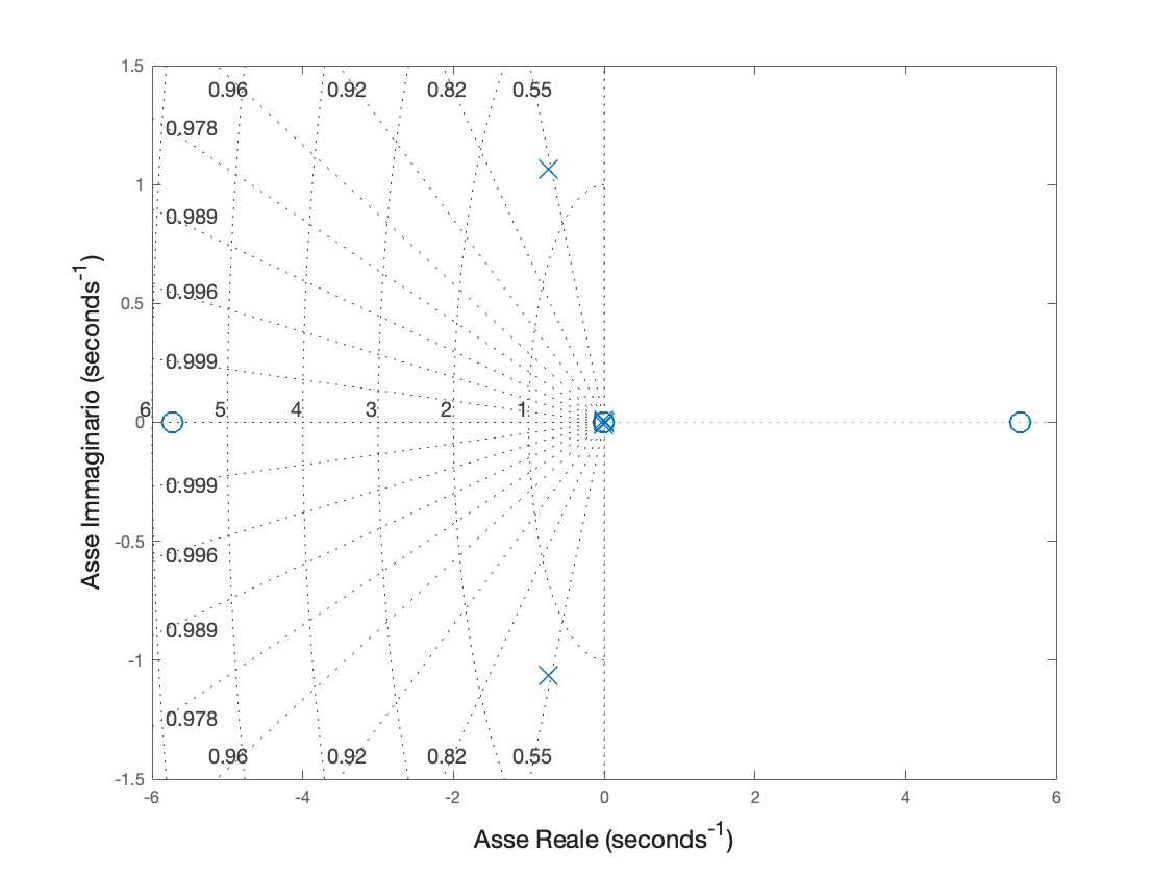
\includegraphics[width=1\linewidth]{Immagini/poli_longitudinali.pdf}
        \captionof{figure}{\texttt{pzplot} dei poli e degli zeri della funzione di trasferimento $W_{\delta_e \rightarrow z}(s)$}
    \end{minipage}
    \hspace{0.02\textwidth}
    \begin{minipage}{.48\textwidth}
        \centering
        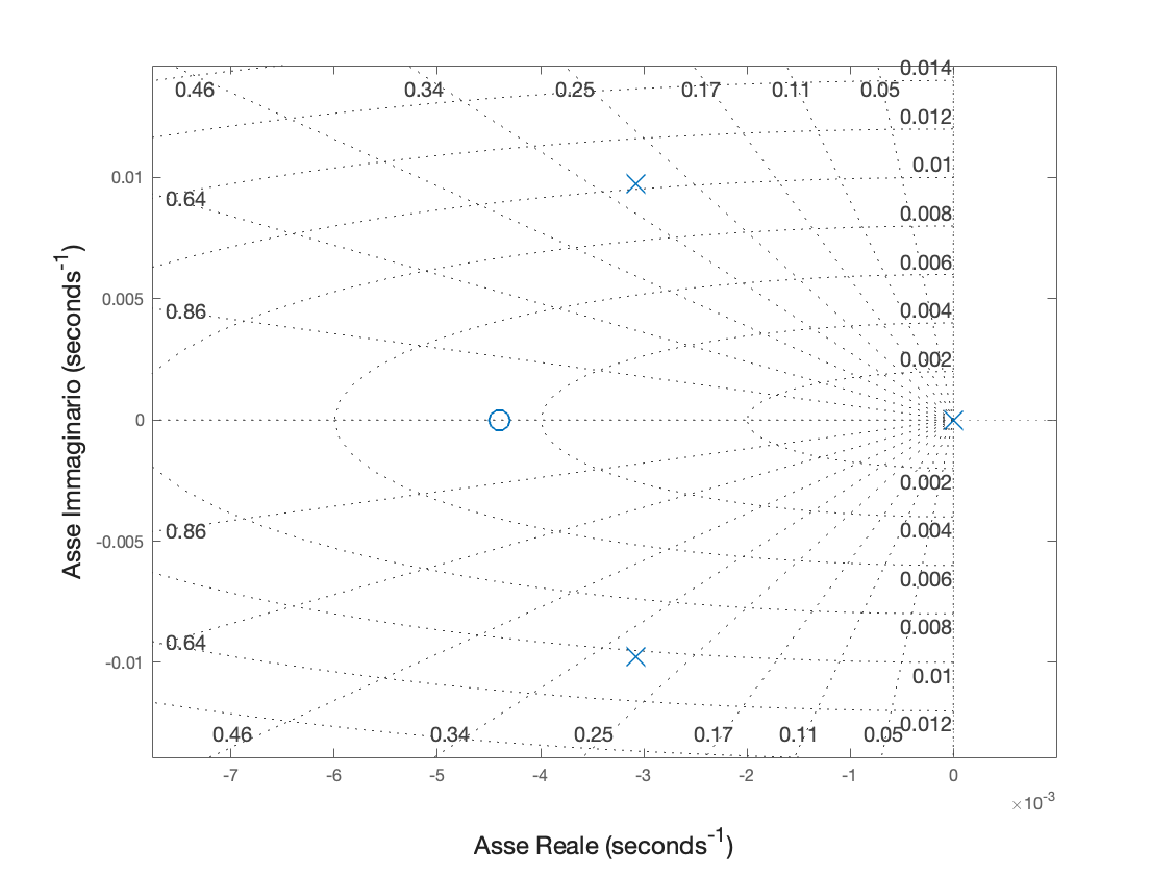
\includegraphics[width=1\linewidth]{Immagini/poli_longitudinali_detail.pdf}
        \captionof{figure}{Dettaglio del grafico vicino all'origine}
    \end{minipage}
\end{figure}


\subsection{Stabilità}

\subsubsection{Stabilità Rispetto alle Condizioni iniziali}

Come definito in \cite{zampieri_dispensa_controlli}:
\begin{sitemize}
    \item un sistema si dice \textbf{asintoticamente stabile} rispetto alle condizioni iniziali quando la sua risposta libera tende a 0: $\lim_{t\to\infty} y_l(t) = 0$.
    \item un sistema si dice \textbf{semplicemente stabile} rispetto alle condizioni iniziali quando la sua risposta libera è limitata : $\left|y_l(t)\right| < M \quad \forall t \geq 0$.
\end{sitemize}

Si può inoltre enunciare il seguente teorema:
\begin{sitemize}
    \item un sistema è \textbf{asintoticamente stabile} rispetto alle condizioni iniziali se e solo se tutte le radici del polinomio caratteristico del sistema ($p_1, p_2, \dots, p_n$) hanno parte reale negativa $Re[p_i] < 0$.
    \item un sistema è \textbf{semplicemente stabile} rispetto alle condizioni iniziali se e solo se tutte le radici del polinomio caratteristico del sistema ($p_1, p_2, \dots, p_n$) hanno parte reale negativa o uguale a $0$ $Re[p_i] \leq 0$.
\end{sitemize}

Il polinomio caratteristico del sistema si può trovare nel denominatore della funzione di trasferimento \eqref{eq:trasferimentoLongitudinali}:
\begin{equation*}
    s(s + 0.73303 \pm j1.0663)(s + 0.0030727 \pm j0.0097528)
\end{equation*}
Le sue radici hanno tutte parte reale minore o uguale a zero, è quindi possibile concludere che il sistema è semplicemente stabile rispetto alle condizioni iniziali.

\subsubsection{BIBO Stabilità}\label{subsubsec:bibo-instabile}

Come definito in \cite{zampieri_dispensa_controlli}:
\begin{sitemize}
    \item un sistema si dice \textbf{BIBO (Bounded Input-Bounded Output) stabile} se ad ogni ingresso limitato, il sistema genera una risposta forzata limitata.
\end{sitemize}

Viene inoltre enunciato il seguente teorema:
\begin{sitemize}
    \item un sistema è \textbf{BIBO stabile} se e solo se la sua funzione di trasferimento ha tutti i poli a parte reale negativa.
\end{sitemize}

Come per la stabilità rispetto alle condizioni iniziali, a causa della presenza di un polo in $s = 0$ a parte reale non negativa il sistema non è BIBO stabile.

L'instabilità del sistema è evidente osservando la risposta al gradino $\delta_e(t) = \delta^{-1}(t)$:

\begin{figure}[H]
    \centering
    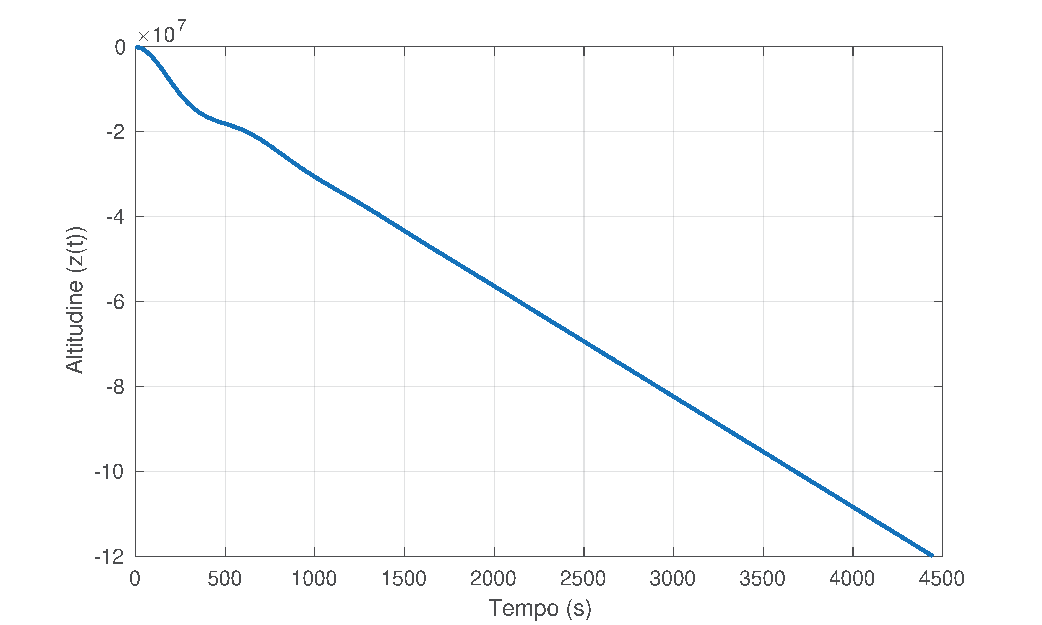
\includegraphics[width=0.65\linewidth]{Immagini/BIBO_instabile.pdf}
\end{figure}

\subsection{Modi Naturali}

La funzione di trasferimento evidenzia, oltre al polo in $s = 0$ che ha dominato la precedente analisi della stabilità, anche due altri poli complessi coniugati.

Un parametro che caratterizza la risposta dinamica di questi poli è il loro coefficiente di smorzamento.
Come si può notare dal grafico, a seconda del valore del coefficiente di smorzamento $\zeta$ si distinguono tre casi:
\begin{sitemize}
    \item quando $\zeta < 1$ il sistema è sottosmorzato, segue quindi un moto oscillatorio.
    \item quando $\zeta = 1$ il sistema è criticamente smorzato, il tempo per ritornare all'equilibrio è in questo caso minimo.
    \item quando $\zeta > 1$ il sistema è sovrasmorzato, ritorna all'equilibrio senza oscillazioni, ma impiega un tempo maggiore del caso precedente.
\end{sitemize}

\begin{figure}[H]
    \centering
    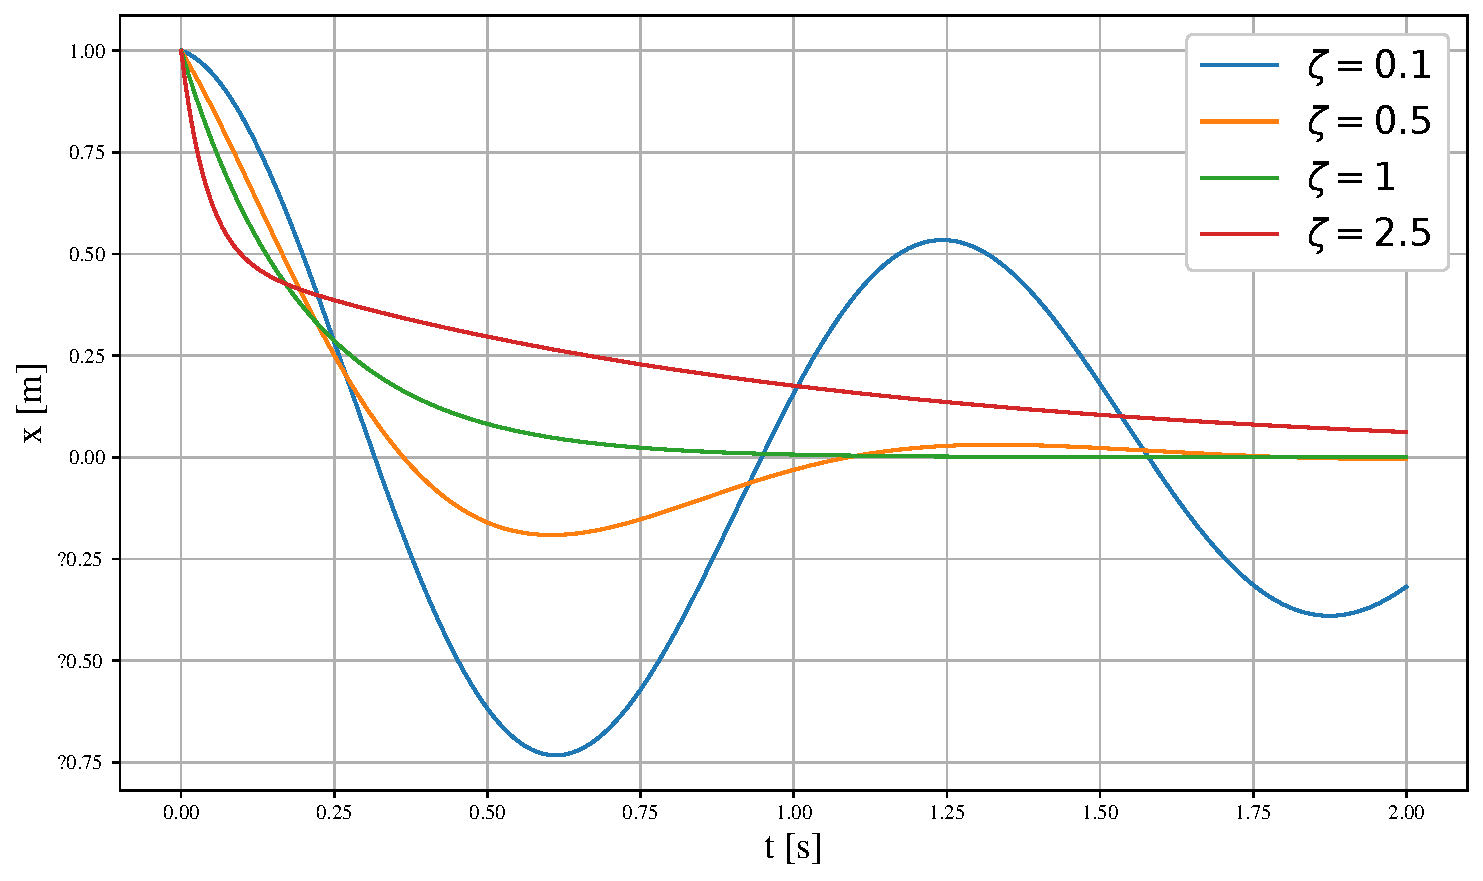
\includegraphics[width=0.65\linewidth]{Immagini/vibrazione_sistema.pdf}
    \caption{Vibrazione di un sistema massa-molla-smorzatore per diversi valori di $\zeta$}
\end{figure}

\subsubsection{Short-Period}\label{subsubsec:short_period}

Il modo associato ai poli in $-0.73303 \pm j1.0663$ è detto \textit{short-period} per la sua breve durata, esso avviene quando il velivolo in volo rettilineo simmetrico uniforme è soggetto ad una raffica di vento verticale o ad un impulso di $\delta_e(t)$.

Il coefficiente di smorzamento e la pulsazione naturale per i poli si calcolano come segue \cite{zampieri_dispensa_controlli}:
\begin{equation*}
    \zeta = - \frac{Re[p]}{\left|p\right|} = 0.5665 \qquad \omega_n = \left|p\right| = 1.2939rad/s
\end{equation*}

Il moto oscillatorio causato da questi poli è fortemente smorzato e quindi di breve durata.

\begin{figure}[H]
    \centering
    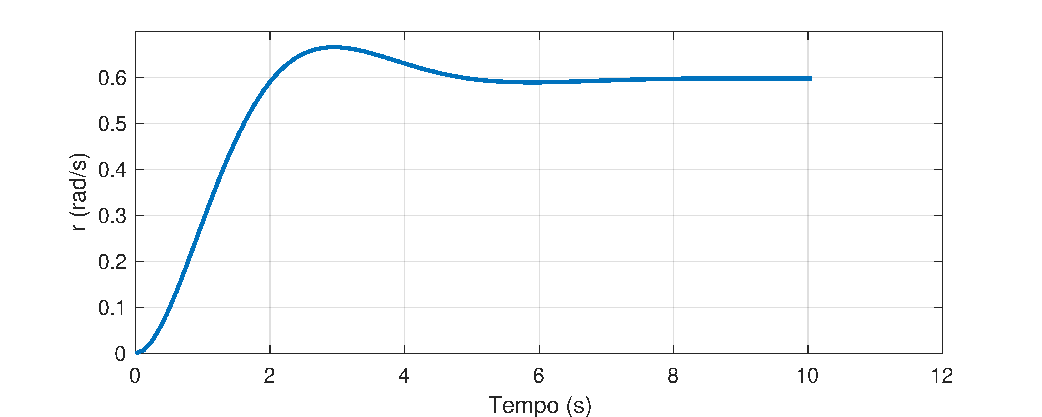
\includegraphics[width=0.7\linewidth]{Immagini/shortperiod_mode.pdf}
    \caption{Risposta impulsiva dei poli assiociati al modo \textit{short-period} assieme al polo nell'origine del Boeing 747 in esame}
\end{figure}

\subsubsection{Phugoid}

Il modo associato ai poli in $-0.0030727 \pm j0.0097528$ è detto \textit{phugoid}, esso avviene quando il velivolo in volo rettilineo simmetrico uniforme è soggetto ad una raffica di vento frontale.
Dopo la raffica di vento si innesca uno scambio tra energia potenziale e cinetica che si protrae per un lungo periodo di tempo.

\begin{figure}[H]
    \centering
    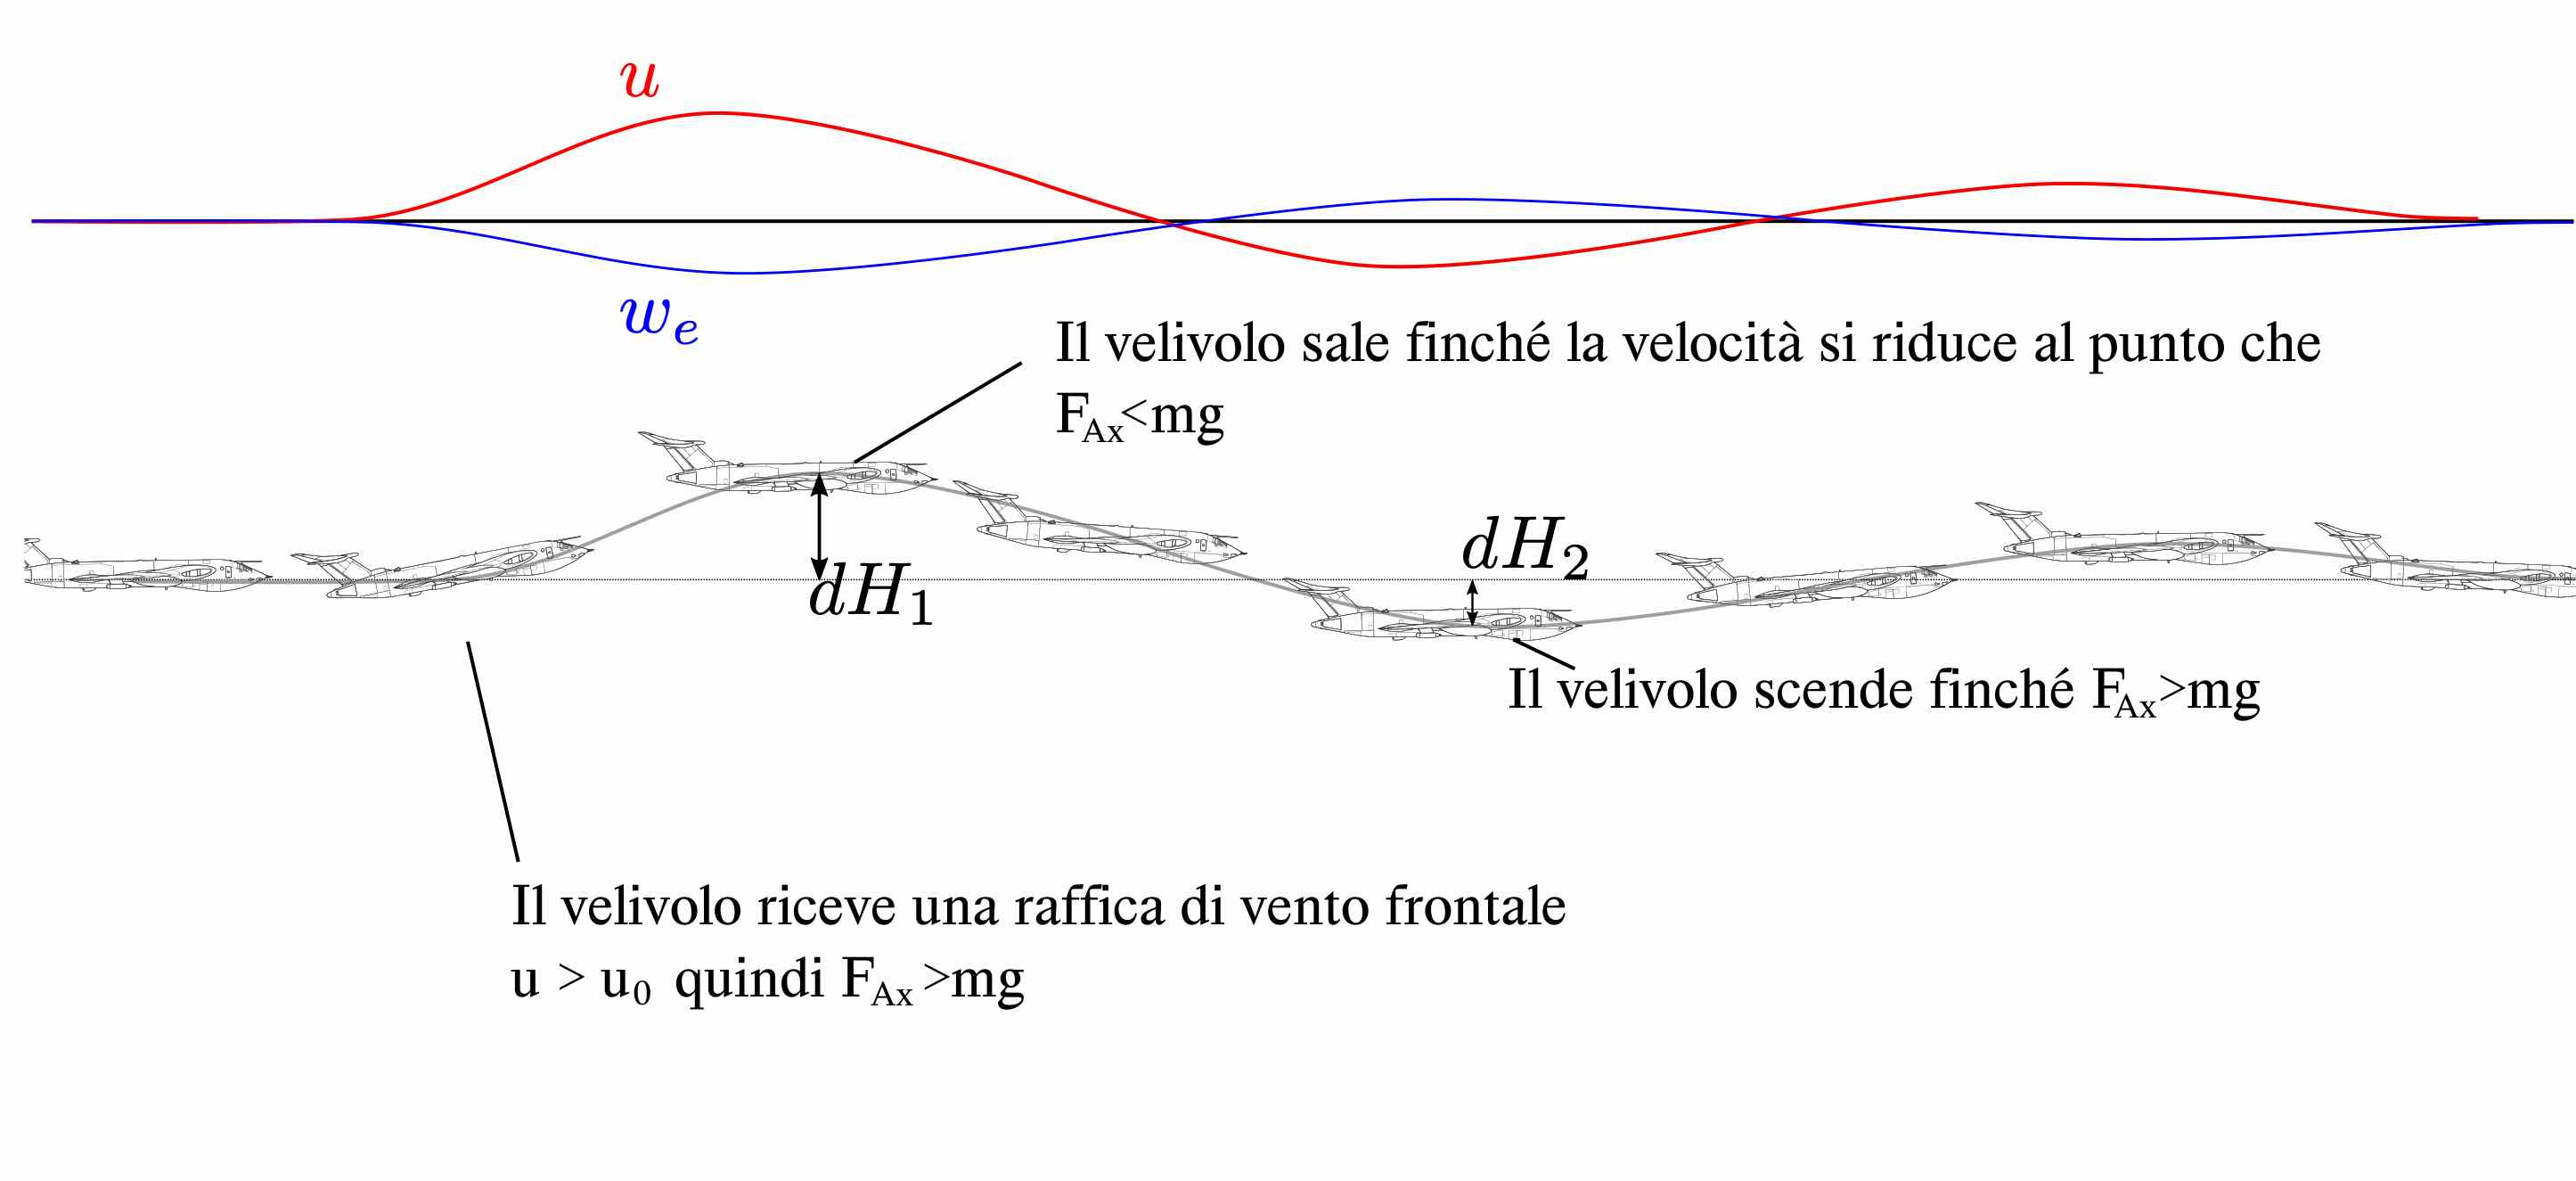
\includegraphics[width=0.9\linewidth]{Immagini/phugoid_mode_physics.jpg}
\end{figure}

In questo caso il coefficiente di smorzamento e la pulsazione naturale per i poli sono:
\begin{equation*}
    \zeta = - \frac{Re[p]}{\left|p\right|} = 0.3005 \qquad \omega_n = \left|p\right| = 0.01022rad/s
\end{equation*}

Si può notare che sia il coefficiente di smorzamento che la pulsazione naturale sono inferiori che nel modo precedente. Il tempo di assestamento è quindi molto maggiore, arrivando fino a 24 minuti per il Boeing 747 in esame.
\begin{figure}[H]
    \centering
    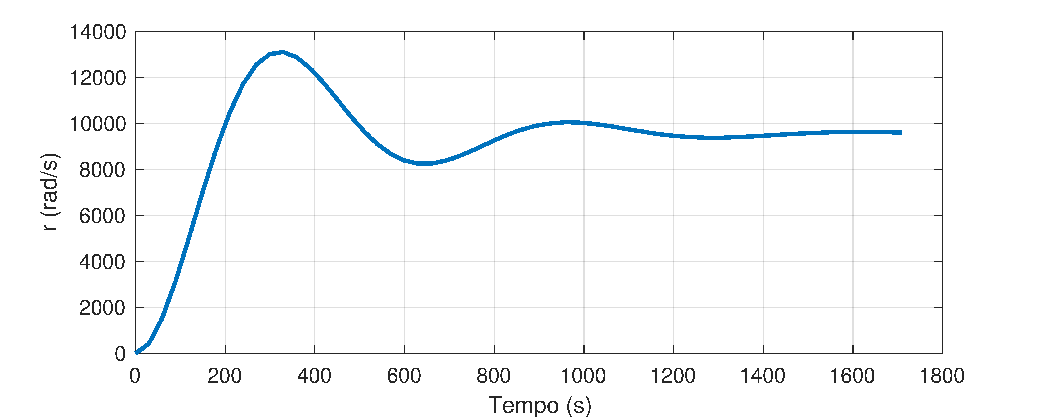
\includegraphics[width=0.7\linewidth]{Immagini/phugoid_mode.pdf}
    \caption{Risposta impulsiva dei poli associati al modo \textit{phugoid} assieme al polo nell'origine  del Boeing 747 in esame}
\end{figure}


\section{Moti Laterali}
I velivoli dotati di ali a freccia positiva, come il Boeing 747, presentano tipicamente un basso smorzamento nei modi laterali.
Tali dinamiche risultano particolarmente difficili da gestire per il pilota, motivo per cui questa tipologia di aeromobili è solitamente equipaggiata con sistemi di controllo automatico volti a supportare e facilitare il lavoro del pilota.

\subsection{Ingressi e Uscite}

I moti laterali oggetto di studio sono influenzati sia dal timone che dagli alettoni. Nel controllo verrà impiegato solamente il timone in quanto ha una maggiore autorità sui moti che si desidera ridurre.

Verrà inoltre utilizzato un giroscopio per misurare l'angolo di imbardata, in quanto particolarmente influenzato dai moti laterali.
\begin{figure}[H]
    \centering
    \begin{tikzpicture}
        \node[draw,
            circle,
            minimum size=0.5cm,
        ] (sum) at (0,0){};

        % Controller
        \node [draw,
            minimum width=2.4cm,
            minimum height=1.2cm,
            right=1.5cm of sum
        ]  (controller) {$Controllore$};

        % System
        \node [draw,
            minimum width=2.4cm,
            minimum height=2.8cm,
            right=1.5cm of controller,
            yshift=0.8cm
        ]  (system) {$Sistema$};

        % Sensor block
        \node [draw,
            minimum width=2.4cm,
            minimum height=1.2cm,
            below right= 1cm and -0.25cm of controller
        ]  (sensor) {$Giroscopio$};


        \draw[-stealth] (system.east) -- ++ (1.5,0)
        node[midway](output){}node[midway,above]{$r$};

        \draw[stealth-] (system.150) -- ++ (-1.5,0)
        node[midway,above]{$\delta_a$};

        \draw[-stealth] (controller.east) -- ++ (1.5,0);

        \draw[-stealth] (sum.east) -- ++ (1.5,0);
        \draw[stealth-] (sum.west) -- ++ (-1.25,0)
        node[midway,above]{$\delta_r$};

        \draw[-stealth] (sensor.west) -| (sum.south);

        \draw[-stealth] (output.center) |- (sensor.east);
    \end{tikzpicture}
\end{figure}

\renewcommand{\arraystretch}{1.2}
\begin{table}[H]
    \begin{tabularx}{\textwidth}{|c|X|}
        \hline
        \multicolumn{2}{|l|}{\textbf{Ingressi}}                                         \\
        \hline
        $\delta_r$ & angolo di deflessione del timone                                   \\
        \hline
        \multicolumn{2}{|l|}{\textbf{Uscite}}                                           \\
        \hline
        $r$        & componente lungo $z_{FRD}$ del vettore $\vec{w}_{FRD}$             \\
        \hline
        \multicolumn{2}{|l|}{\textbf{Variabili di Stato}}                               \\
        \hline
        $p$, $r$   & componenti lungo $x_{FRD}$ e $z_{FRD}$ del vettore $\vec{w}_{FRD}$ \\
        $\beta$    & angolo di derapata                                                 \\
        $\phi$     & angolo di rollio                                                   \\
        \hline
    \end{tabularx}
\end{table}

\subsection{Funzione di Trasferimento}
Utilizzando la funzione \texttt{ss2tf} di MATLAB sul modello di stato \eqref{eq:motoLaterale} si ottiene la funzione di trasferimento:

\begin{equation}
    \label{eq:trasferimentoLaterali}
    \begin{split}
        W_{\delta_r \rightarrow r}(s) & = \frac{-0.475 s^3 - 0.24789 s^2 - 0.11871 s - 0.056462}{s^4 + 0.6358 s^3 + 0.94078 s^2 + 0.51313 s + 0.003683} \\
                                      & = -0.475\frac{(s + 0.4987)(s + 0.0116 \pm j0.4881)}{(s + 0.5630)(s + 0.0073)(s + 0.0328 \pm j0.9478)}
    \end{split}
\end{equation}

Dalla forma di Evans \cite{zampieri_dispensa_controlli}, riportata nella seconda riga, è possibile individuare i poli e gli zeri. In particolare sono presenti tre zeri, $s = -0.4987, s = - 0.0116 \pm j0.4881$, e quattro poli, $s = -0.5630, s = -0.0073, s = -0.0328 \pm j0.9478$

\begin{figure}[H]
    \centering
    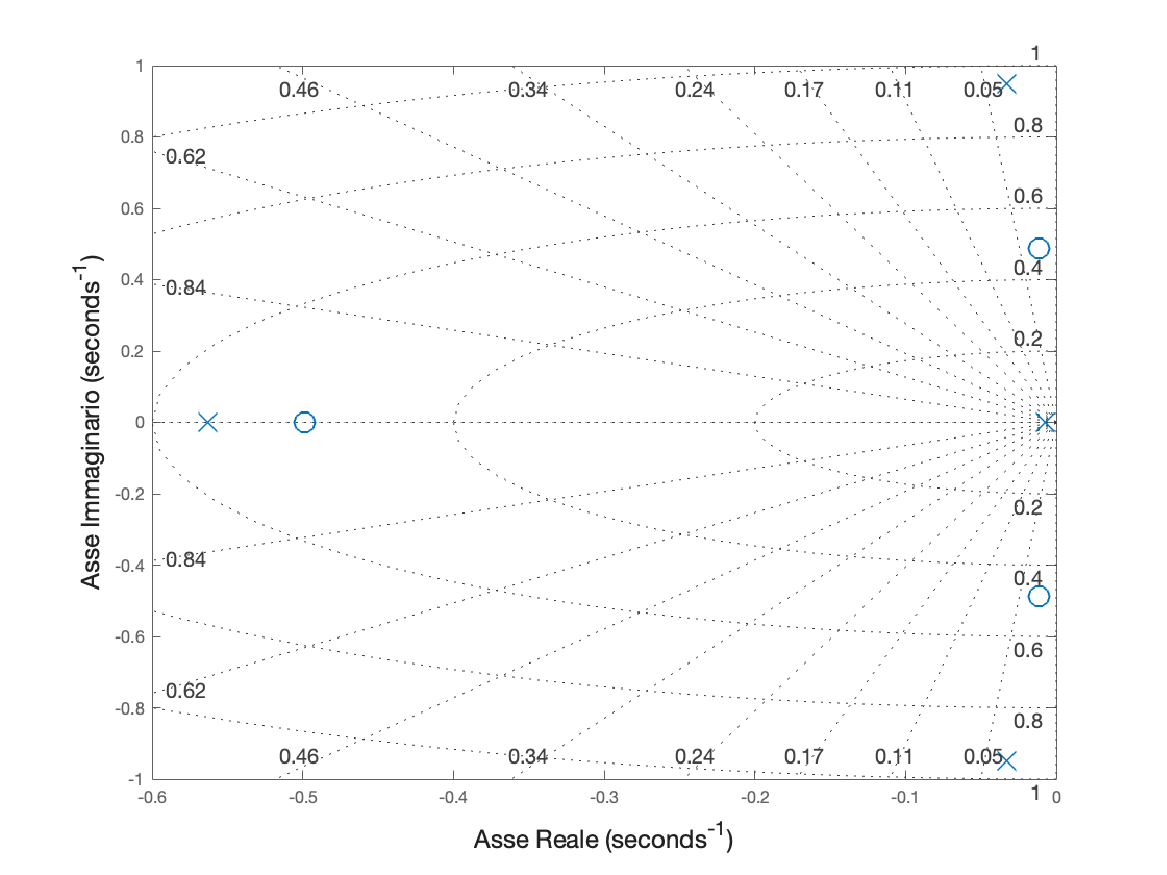
\includegraphics[width=0.7\linewidth]{Immagini/poli_laterali.pdf}
    \caption{\texttt{pzplot} dei poli e degli zeri della funzione di trasferimento $ W_{\delta_r \rightarrow r}(s)$}
\end{figure}

\subsection{Stabilità}

\subsubsection{Stabilità Rispetto alle Condizioni iniziali}

Il polinomio caratteristico del sistema è:
\begin{equation*}
    (s + 0.5630)(s + 0.0073)(s + 0.0328 \pm j0.9478)
\end{equation*}
Le sue radici hanno tutte parte reale $< 0$, è quindi possibile concludere che il sistema è asintoticamente stabile rispetto alle condizioni iniziali.

\subsubsection{BIBO Stabilità}

La funzione di trasferimento ha tutti i poli a parte reale negativa, si conclude che il sistema è BIBO stabile.

\subsection{Modi Naturali}

In questo caso la funzione di trasferimento è costituita da quattro poli: due reali e due complessi coniugati.

I poli reali danno origine a modi criticamente smorzati ($\zeta = 1$), mentre i poli complessi coniugati generano un moto oscillatorio denominato \textit{dutch roll}.

\subsubsection{Spiral}

Il modo associato al polo in $-0.0073$ è detto \textit{spiral}. Esso si manifesta quando, a seguito di una perturbazione, il velivolo acquisisce un angolo di rollio $\phi > 0$.
A seguito della perturbazione la coda del velivolo inizia a generare una componente di portanza, che tende ad aumentare ulteriormente l'angolo $\phi$.

In base all'entità della forza generata, il velivolo può ritornare lentamente alla sua posizione iniziale, come nel caso del Boeing 747, oppure può entrare in una virata di raggio decrescente che può condurre a una pericolosa situazione nota come \textit{graveyard spiral}.

\begin{figure}[H]
    \centering
    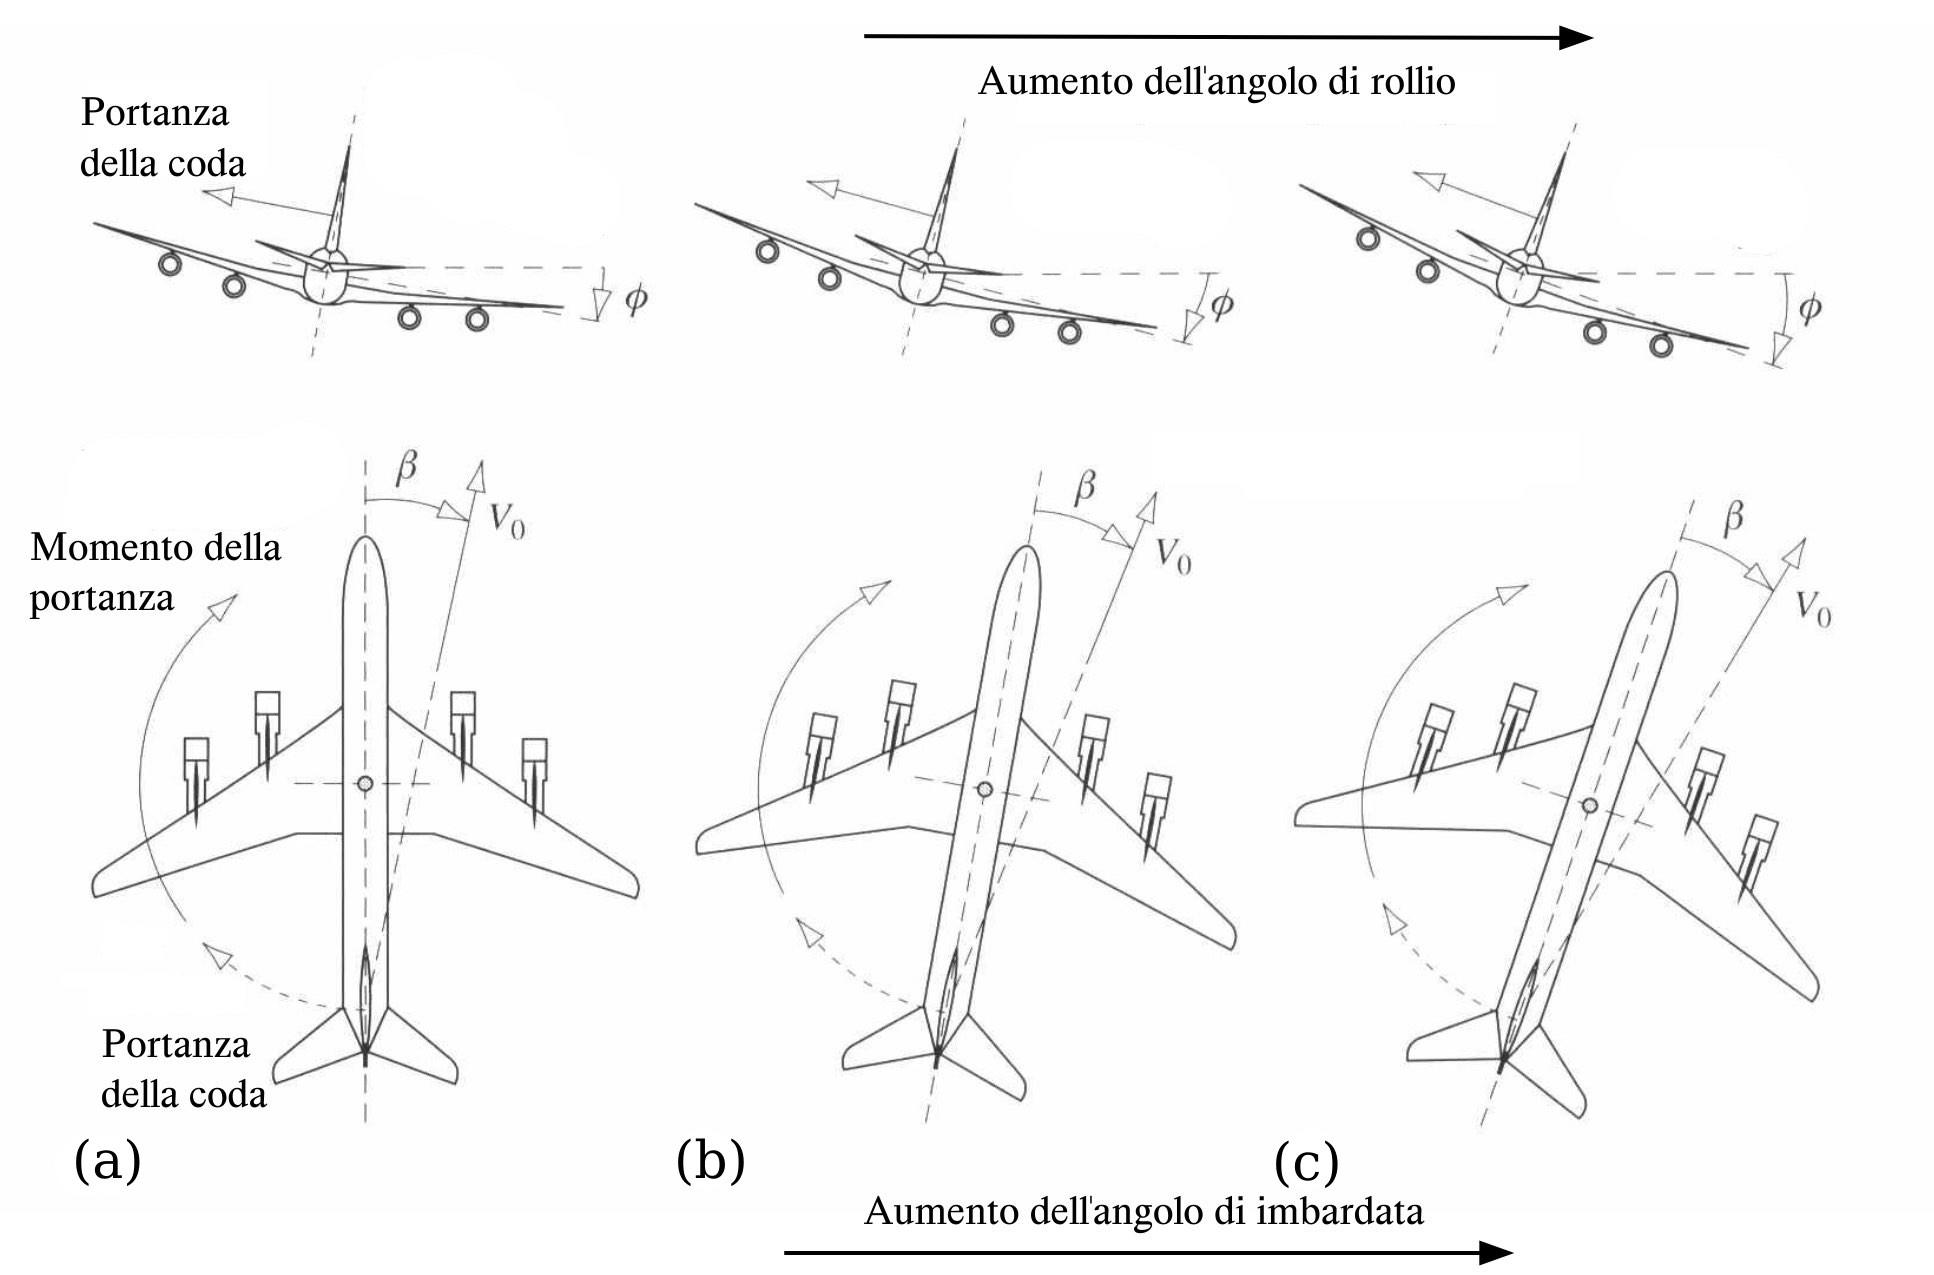
\includegraphics[width=0.8\linewidth]{Immagini/spiral_mode_physics.jpg}
    \caption{Influenza della portanza della coda sull'angolo di rollio e di imbardata \cite{cook1997flight}}
\end{figure}

Dal calcolo del coefficiente di smorzamento e della pulsazione naturale si può osservare come questo modo sia di lungo periodo:
\begin{equation*}
    \zeta = - \frac{Re[p]}{\left|p\right|} = 1 \qquad \omega_n = \left|p\right| = 0.0073rad/s
\end{equation*}

\begin{figure}[H]
    \centering
    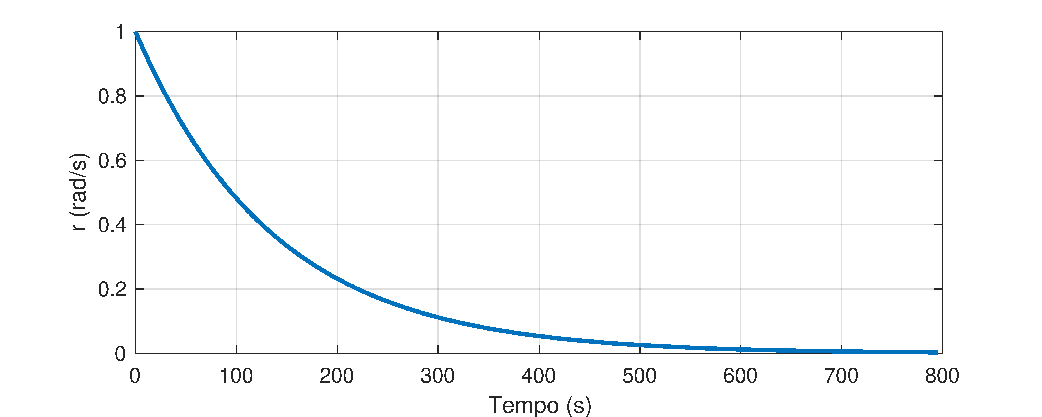
\includegraphics[width=0.7\linewidth]{Immagini/spiral_mode.pdf}
    \caption{Risposta impulsiva per il polo associato al modo \textit{spiral} del Boeing 747 in esame}
\end{figure}

\subsubsection{Roll}

Il modo associato al polo in $-0.5630$ è detto \textit{roll}. Esso si verifica quando il velivolo ruota attorno all'asse $\hat{x}_{FRD}$, ovvero quando la velocità angolare $p$ subisce una variazione.

In questo caso il modo è ben smorzato, quindi il velivolo ritorna rapidamente alla sua condizione di equilibrio dopo una perturbazione.

Ciò è confermato anche dal valore del coefficiente di smorzamento e della pulsazione naturale:
\begin{equation*}
    \zeta = - \frac{Re[p]}{\left|p\right|} = 1 \qquad \omega_n = \left|p\right| = 0.5630rad/s
\end{equation*}

\begin{figure}[H]
    \centering
    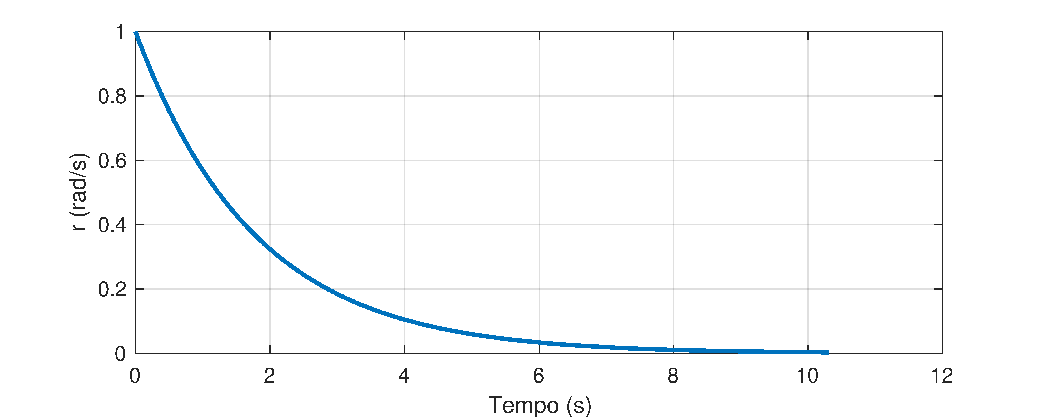
\includegraphics[width=0.7\linewidth]{Immagini/roll_mode.pdf}
    \caption{Risposta impulsiva per il polo associato al modo \textit{roll} del Boeing 747 in esame}
\end{figure}

\subsubsection{Dutch Roll}

Il modo associato ai poli in $-0.0328 \pm j0.9478$ è detto \textit{dutch roll} ed è caratterizzato da un moto oscillatorio che coinvolge simultaneamente rollio, imbardata e derapata.

In particolare, può iniziare con un incremento dell'angolo di imbardata $\psi$, che provoca una variazione dell'incidenza relativa sulle due ali: l'ala avanzata genera una maggiore portanza rispetto all'altra.
Questo squilibrio induce un aumento dell'angolo di rollio $\phi$, che a sua volta altera la direzione del moto e innesca un'imbardata in senso opposto.
Il ciclo si ripete, dando luogo a un'oscillazione di lungo periodo.

\begin{figure}[H]
    \centering
    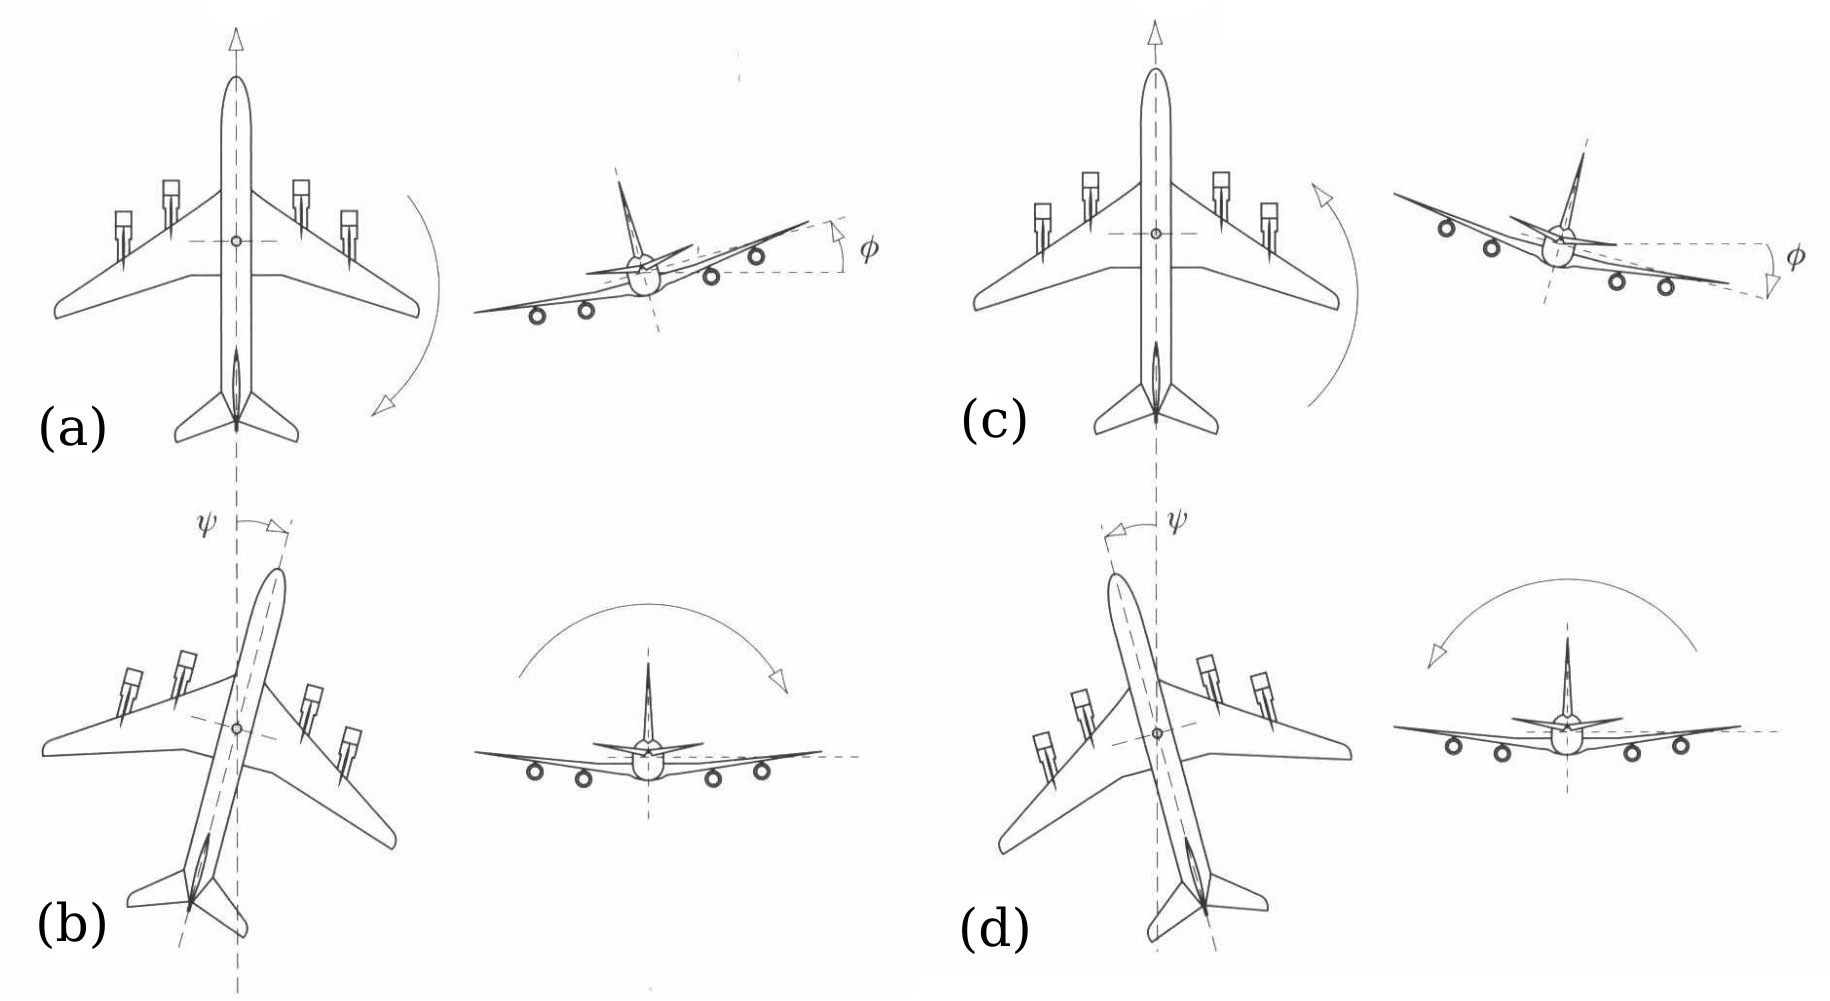
\includegraphics[width=0.8\linewidth]{Immagini/dutch_roll_physics.jpg}
    \caption{Interazione tra gli angoli di rollio e di imbardata \cite{cook1997flight}}
\end{figure}

I parametri del coefficiente di smorzamento e della pulsazione naturale sono:
\begin{equation*}
    \zeta = - \frac{Re[p]}{\left|p\right|} = 0.034585 \qquad \omega_n = \left|p\right| = 0.94836
\end{equation*}

\begin{figure}[H]
    \centering
    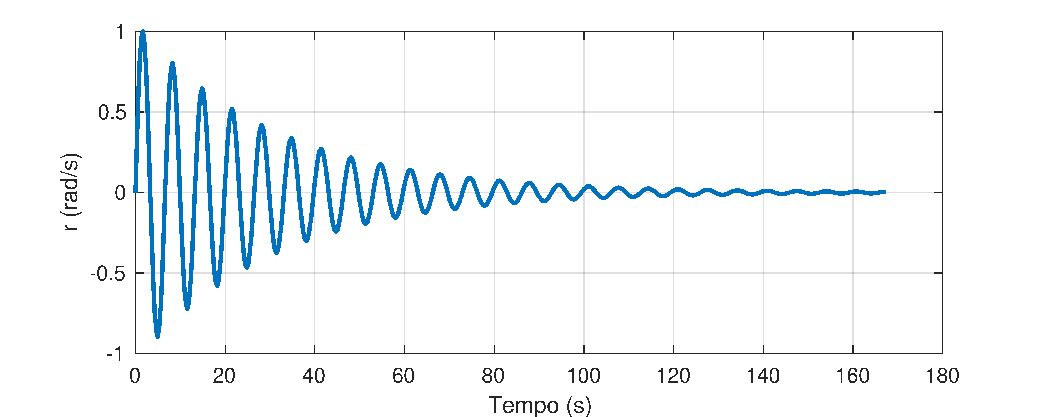
\includegraphics[width=0.7\linewidth]{Immagini/dutch_roll_mode.pdf}
    \caption{Risposta impulsiva per i poli associati al modo \textit{dutch roll} del Boeing 747 in esame}
\end{figure}

\chapter{Controllo}
\section{Moti Longitudinali}
Vengono ora analizzati i moti longitudinali del sistema, analisi che sarà successivamente impiegata per stabilizzare il sistema e per sviluppare un autopilota in grado di mantenere una determinata altitudine di volo.

Uno dei compiti del pilota di un velivolo è quello di mantenere una determinata quota, al fine di evitare potenziali collisioni con altri aeromobili.
Un pilota ben addestrato e attento è in grado di svolgere questo compito manualmente con una precisione di $\pm 50$ ft; per tale motivo i controllori del traffico aereo si aspettano che tale tolleranza venga rispettata.

Poiché questo compito richiede un elevato livello di attenzione e diligenza, gli aeromobili più sofisticati sono spesso dotati di un autopilota per il mantenimento della quota, così da ridurre il carico di lavoro del pilota.

\subsection{Ingressi e Uscite}

Il controllo dell'altitudine verrà effettuato agendo esclusivamente sugli equilibratori; la forza propulsiva non viene modificata dal controllore.

A tal fine, viene utilizzato un altimetro barometrico per la misura dell'altitudine del velivolo, strumento comunemente impiegato nei sistemi avionici per stimare la quota in base alla pressione atmosferica.

\begin{figure}[H]
    \centering
    \begin{tikzpicture}
        \node[draw,
            circle,
            minimum size=0.5cm,
        ] (sum) at (0,0){};

        % Controller
        \node [draw,
            minimum width=2.4cm,
            minimum height=1.2cm,
            right=1.5cm of sum
        ]  (controller) {$Controllore$};

        % System
        \node [draw,
            minimum width=2.4cm,
            minimum height=2.8cm,
            right=1.5cm of controller,
            yshift=0.8cm
        ]  (system) {$Sistema$};

        % Sensor block
        \node [draw,
            minimum width=2.4cm,
            minimum height=1.2cm,
            below right= 1cm and -0.25cm of controller
        ]  (sensor) {$Altimetro$};


        \draw[-stealth] (system.east) -- ++ (1.5,0)
        node[midway](output){}node[midway,above]{$z$};

        \draw[stealth-] (system.150) -- ++ (-1.5,0)
        node[midway,above]{$\delta_t$};

        \draw[-stealth] (controller.east) -- ++ (1.5,0);

        \draw[-stealth] (sum.east) -- ++ (1.5,0);
        \draw[stealth-] (sum.west) -- ++ (-1.25,0)
        node[midway,above]{$\delta_e$};

        \draw[-stealth] (sensor.west) -| (sum.south);

        \draw[-stealth] (output.center) |- (sensor.east);
    \end{tikzpicture}
\end{figure}

\renewcommand{\arraystretch}{1.2}
\begin{table}[H]
    \begin{tabularx}{\textwidth}{|c|X|}
        \hline
        \multicolumn{2}{|l|}{\textbf{Ingressi}}                                          \\
        \hline
        $\delta_e$ & angolo di deflessione degli equilibratori                           \\
        \hline
        \multicolumn{2}{|l|}{\textbf{Uscite}}                                            \\
        \hline
        $z$        & Variazione dell'altitudine rispetto al valore iniziale di 20.000 ft \\
        \hline
        \multicolumn{2}{|l|}{\textbf{Variabili di Stato}}                                \\
        \hline
        $u$, $w$   & componenti lungo $x_{FRD}$ e $z_{FRD}$ del vettore $\vec{V}_{FRD}$  \\
        $q$        & componente lungo $y_{FRD}$ del vettore $\vec{w}_{FRD}$              \\
        $\theta$   & angolo di beccheggio                                                \\
        $z$        & Variazione dell'altitudine rispetto al valore iniziale di 20.000 ft \\
        \hline
    \end{tabularx}
\end{table}

\subsection{Funzione di Trasferimento}
Utilizzando la funzione \texttt{ss2tf} di MATLAB sul modello di stato \eqref{eq:motoLongitudinale} si ottiene la funzione di trasferimento:

\begin{equation}
    \label{eq:trasferimentoLongitudinali}
    \begin{split}
        W_{\delta_e \rightarrow z}(s) & = \frac{32.7 s^3 + 7.0486 s^2 - 1035.7 s - 4.5535}{s^5 + 1.4722 s^4 + 1.6835 s^3 + 0.010443 s^2 + 0.00017507 s} \\
                                      & = 32.7\frac{(s + 0.0043964)(s - 5.5234)(s + 5.7345)}{s(s + 0.73303 \pm j1.0663)(s + 0.0030727 \pm j0.0097528)}
    \end{split}
\end{equation}

Dalla forma di Evans \cite{zampieri_dispensa_controlli}, riportata nella seconda riga, è possibile individuare i poli e gli zeri. In particolare sono presenti tre zeri, $s = -0.0043964, s = 5.5234, s = - 5.7345$, e cinque poli, $s = 0, s = -0.73303 \pm j1.0663, s = -0.0030727 \pm j0.0097528$

\begin{figure}[H]
    \centering
    \begin{minipage}{.48\textwidth}
        \centering
        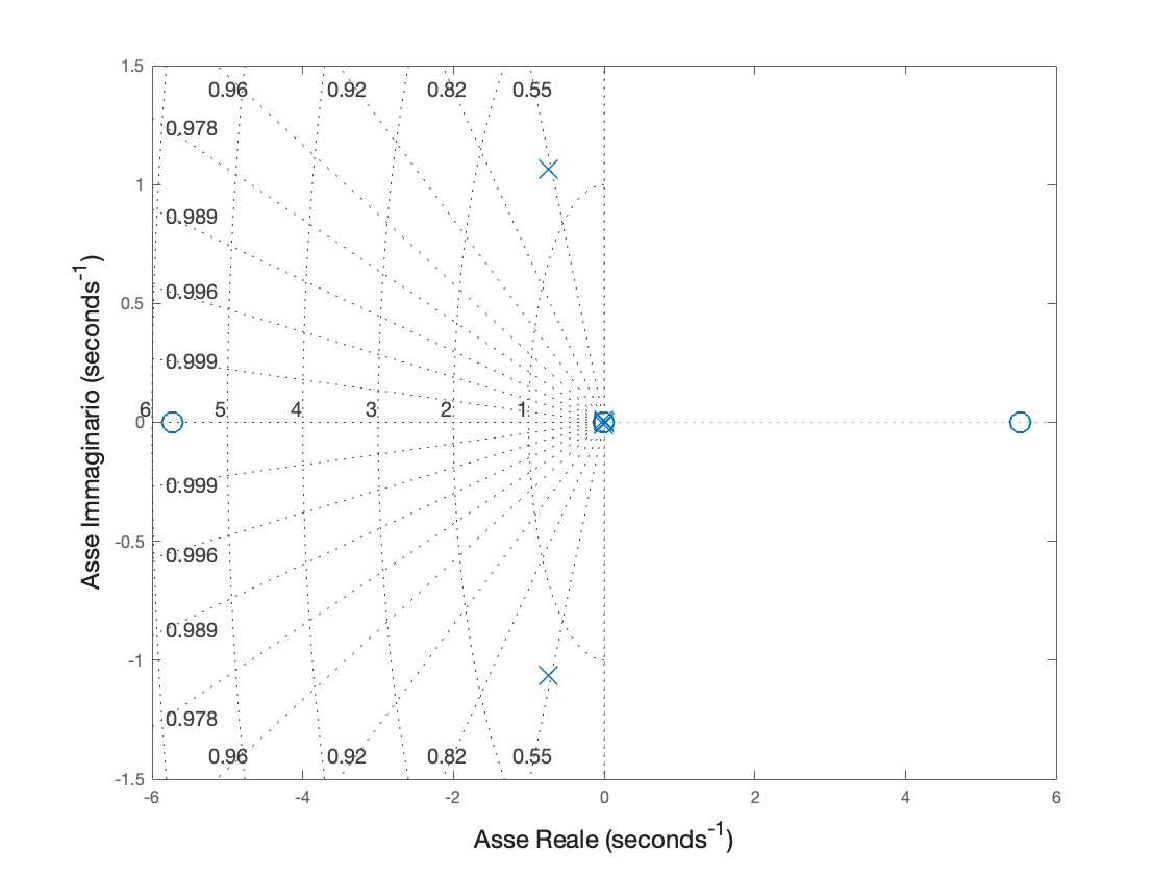
\includegraphics[width=1\linewidth]{Immagini/poli_longitudinali.pdf}
        \captionof{figure}{\texttt{pzplot} dei poli e degli zeri della funzione di trasferimento $W_{\delta_e \rightarrow z}(s)$}
    \end{minipage}
    \hspace{0.02\textwidth}
    \begin{minipage}{.48\textwidth}
        \centering
        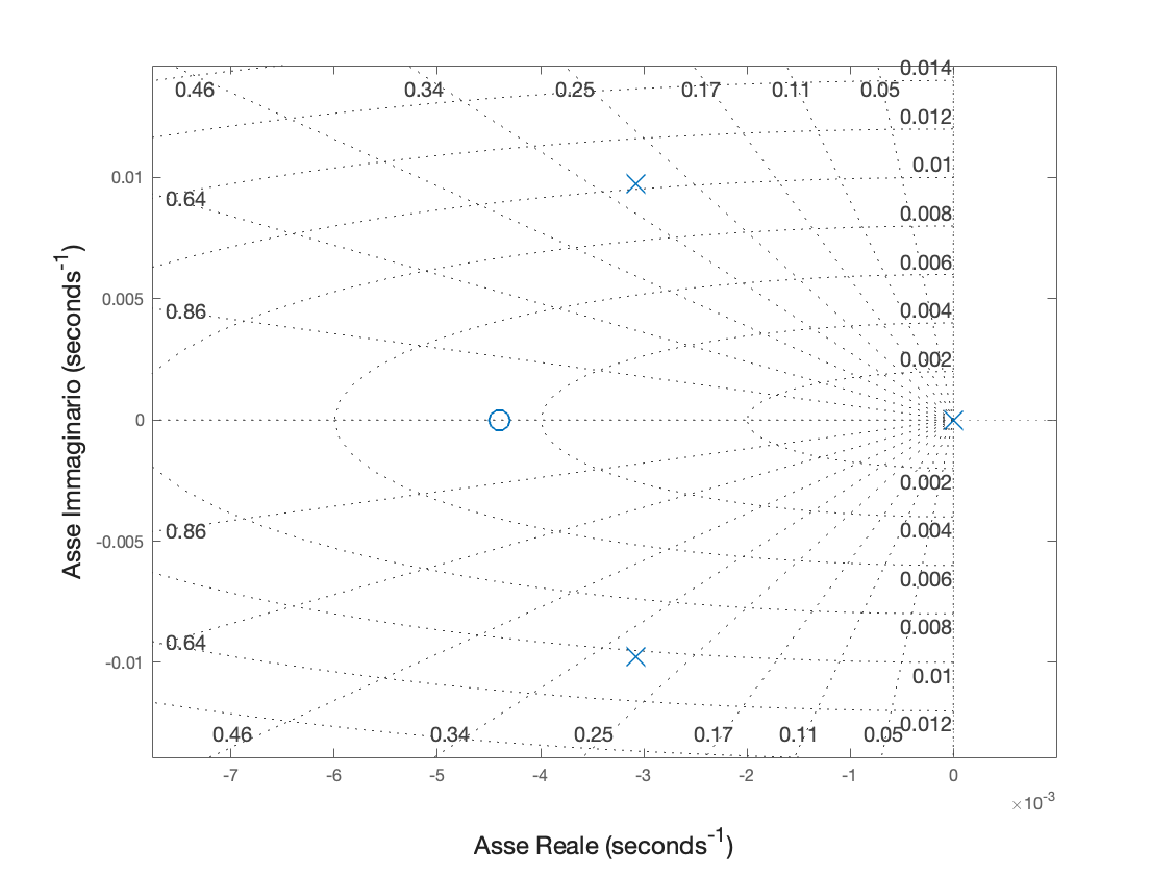
\includegraphics[width=1\linewidth]{Immagini/poli_longitudinali_detail.pdf}
        \captionof{figure}{Dettaglio del grafico vicino all'origine}
    \end{minipage}
\end{figure}


\subsection{Stabilità}

\subsubsection{Stabilità Rispetto alle Condizioni iniziali}

Come definito in \cite{zampieri_dispensa_controlli}:
\begin{sitemize}
    \item un sistema si dice \textbf{asintoticamente stabile} rispetto alle condizioni iniziali quando la sua risposta libera tende a 0: $\lim_{t\to\infty} y_l(t) = 0$.
    \item un sistema si dice \textbf{semplicemente stabile} rispetto alle condizioni iniziali quando la sua risposta libera è limitata : $\left|y_l(t)\right| < M \quad \forall t \geq 0$.
\end{sitemize}

Si può inoltre enunciare il seguente teorema:
\begin{sitemize}
    \item un sistema è \textbf{asintoticamente stabile} rispetto alle condizioni iniziali se e solo se tutte le radici del polinomio caratteristico del sistema ($p_1, p_2, \dots, p_n$) hanno parte reale negativa $Re[p_i] < 0$.
    \item un sistema è \textbf{semplicemente stabile} rispetto alle condizioni iniziali se e solo se tutte le radici del polinomio caratteristico del sistema ($p_1, p_2, \dots, p_n$) hanno parte reale negativa o uguale a $0$ $Re[p_i] \leq 0$.
\end{sitemize}

Il polinomio caratteristico del sistema si può trovare nel denominatore della funzione di trasferimento \eqref{eq:trasferimentoLongitudinali}:
\begin{equation*}
    s(s + 0.73303 \pm j1.0663)(s + 0.0030727 \pm j0.0097528)
\end{equation*}
Le sue radici hanno tutte parte reale minore o uguale a zero, è quindi possibile concludere che il sistema è semplicemente stabile rispetto alle condizioni iniziali.

\subsubsection{BIBO Stabilità}\label{subsubsec:bibo-instabile}

Come definito in \cite{zampieri_dispensa_controlli}:
\begin{sitemize}
    \item un sistema si dice \textbf{BIBO (Bounded Input-Bounded Output) stabile} se ad ogni ingresso limitato, il sistema genera una risposta forzata limitata.
\end{sitemize}

Viene inoltre enunciato il seguente teorema:
\begin{sitemize}
    \item un sistema è \textbf{BIBO stabile} se e solo se la sua funzione di trasferimento ha tutti i poli a parte reale negativa.
\end{sitemize}

Come per la stabilità rispetto alle condizioni iniziali, a causa della presenza di un polo in $s = 0$ a parte reale non negativa il sistema non è BIBO stabile.

L'instabilità del sistema è evidente osservando la risposta al gradino $\delta_e(t) = \delta^{-1}(t)$:

\begin{figure}[H]
    \centering
    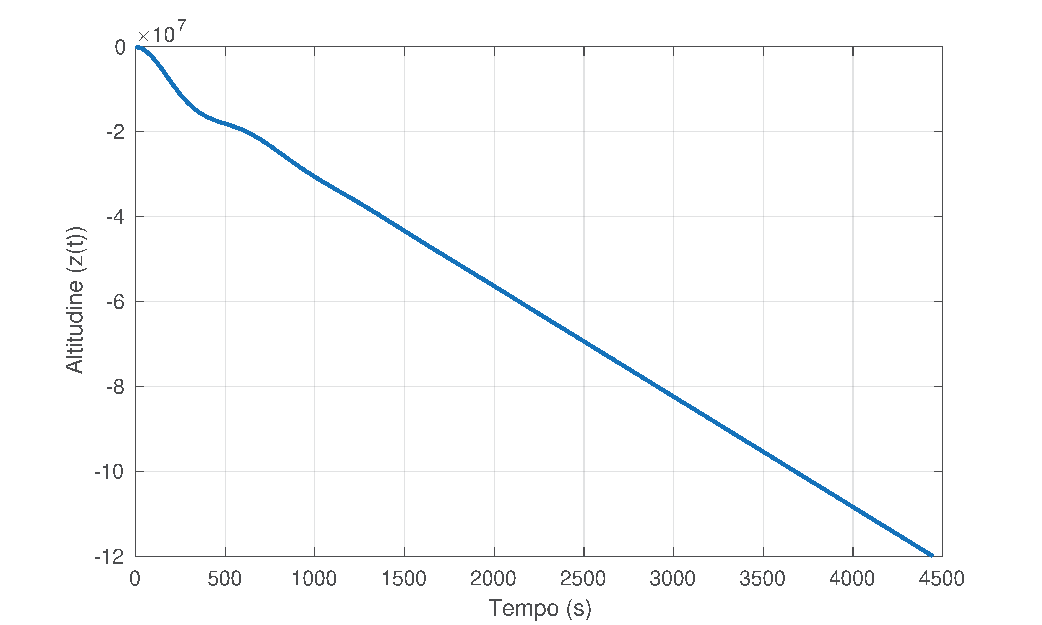
\includegraphics[width=0.65\linewidth]{Immagini/BIBO_instabile.pdf}
\end{figure}

\subsection{Modi Naturali}

La funzione di trasferimento evidenzia, oltre al polo in $s = 0$ che ha dominato la precedente analisi della stabilità, anche due altri poli complessi coniugati.

Un parametro che caratterizza la risposta dinamica di questi poli è il loro coefficiente di smorzamento.
Come si può notare dal grafico, a seconda del valore del coefficiente di smorzamento $\zeta$ si distinguono tre casi:
\begin{sitemize}
    \item quando $\zeta < 1$ il sistema è sottosmorzato, segue quindi un moto oscillatorio.
    \item quando $\zeta = 1$ il sistema è criticamente smorzato, il tempo per ritornare all'equilibrio è in questo caso minimo.
    \item quando $\zeta > 1$ il sistema è sovrasmorzato, ritorna all'equilibrio senza oscillazioni, ma impiega un tempo maggiore del caso precedente.
\end{sitemize}

\begin{figure}[H]
    \centering
    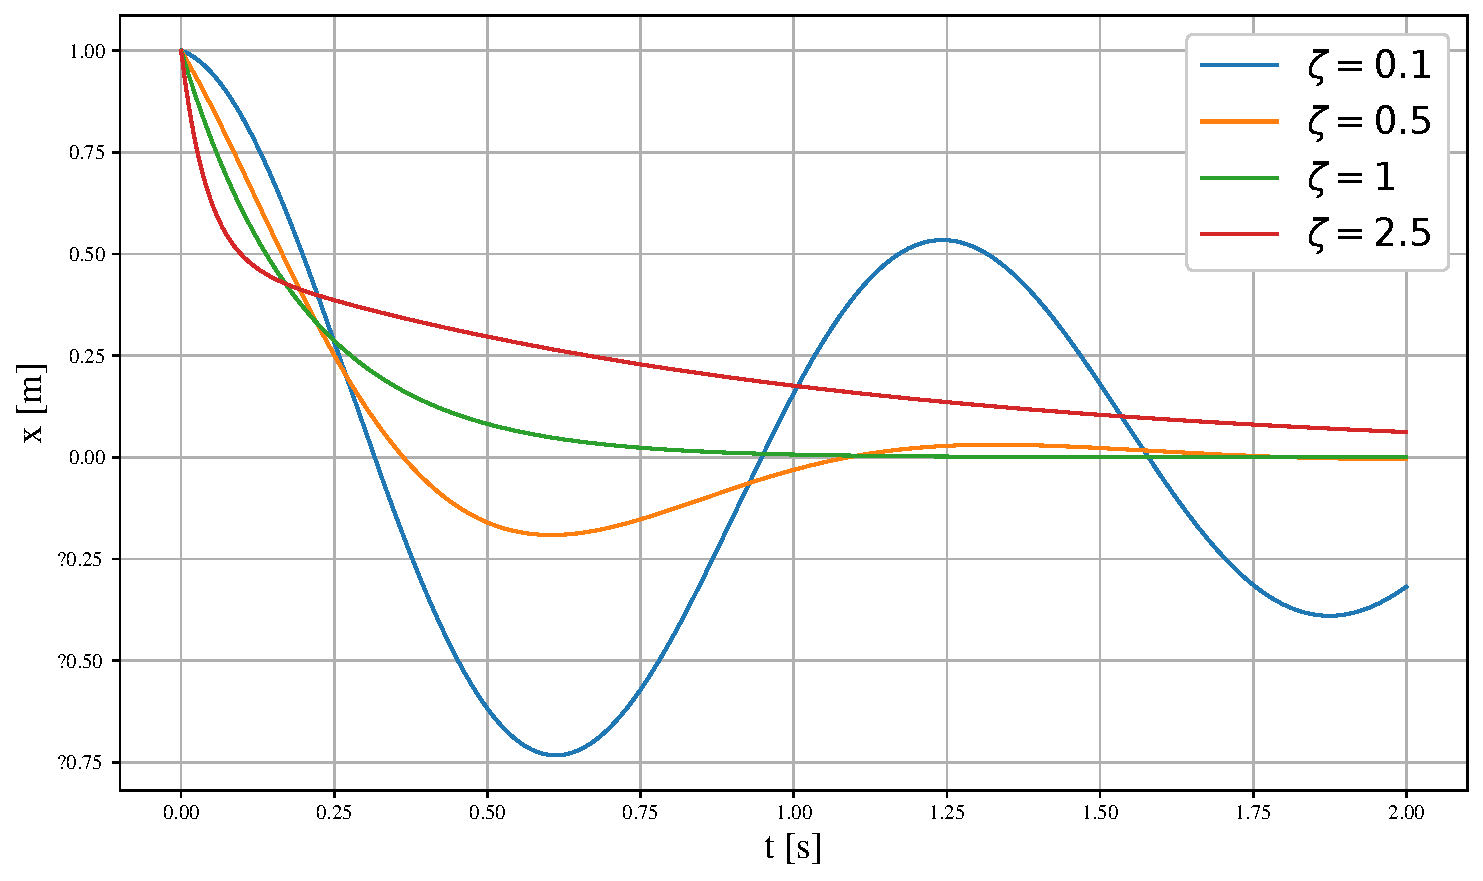
\includegraphics[width=0.65\linewidth]{Immagini/vibrazione_sistema.pdf}
    \caption{Vibrazione di un sistema massa-molla-smorzatore per diversi valori di $\zeta$}
\end{figure}

\subsubsection{Short-Period}\label{subsubsec:short_period}

Il modo associato ai poli in $-0.73303 \pm j1.0663$ è detto \textit{short-period} per la sua breve durata, esso avviene quando il velivolo in volo rettilineo simmetrico uniforme è soggetto ad una raffica di vento verticale o ad un impulso di $\delta_e(t)$.

Il coefficiente di smorzamento e la pulsazione naturale per i poli si calcolano come segue \cite{zampieri_dispensa_controlli}:
\begin{equation*}
    \zeta = - \frac{Re[p]}{\left|p\right|} = 0.5665 \qquad \omega_n = \left|p\right| = 1.2939rad/s
\end{equation*}

Il moto oscillatorio causato da questi poli è fortemente smorzato e quindi di breve durata.

\begin{figure}[H]
    \centering
    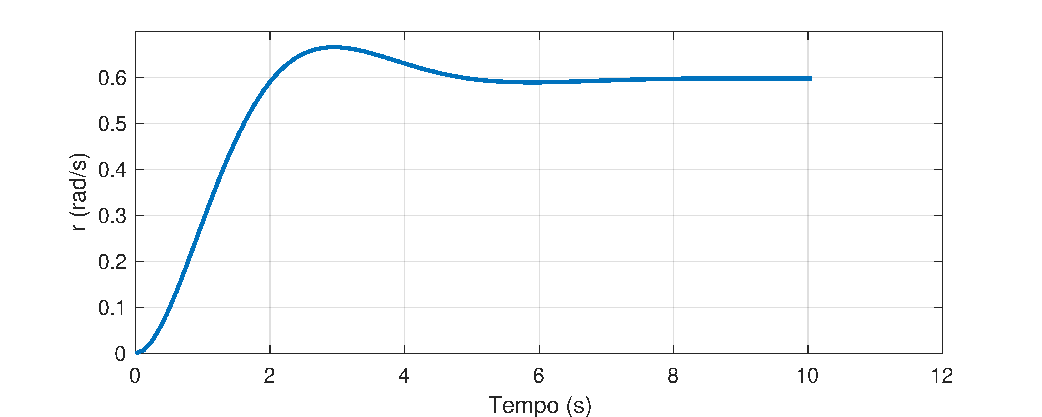
\includegraphics[width=0.7\linewidth]{Immagini/shortperiod_mode.pdf}
    \caption{Risposta impulsiva dei poli assiociati al modo \textit{short-period} assieme al polo nell'origine del Boeing 747 in esame}
\end{figure}

\subsubsection{Phugoid}

Il modo associato ai poli in $-0.0030727 \pm j0.0097528$ è detto \textit{phugoid}, esso avviene quando il velivolo in volo rettilineo simmetrico uniforme è soggetto ad una raffica di vento frontale.
Dopo la raffica di vento si innesca uno scambio tra energia potenziale e cinetica che si protrae per un lungo periodo di tempo.

\begin{figure}[H]
    \centering
    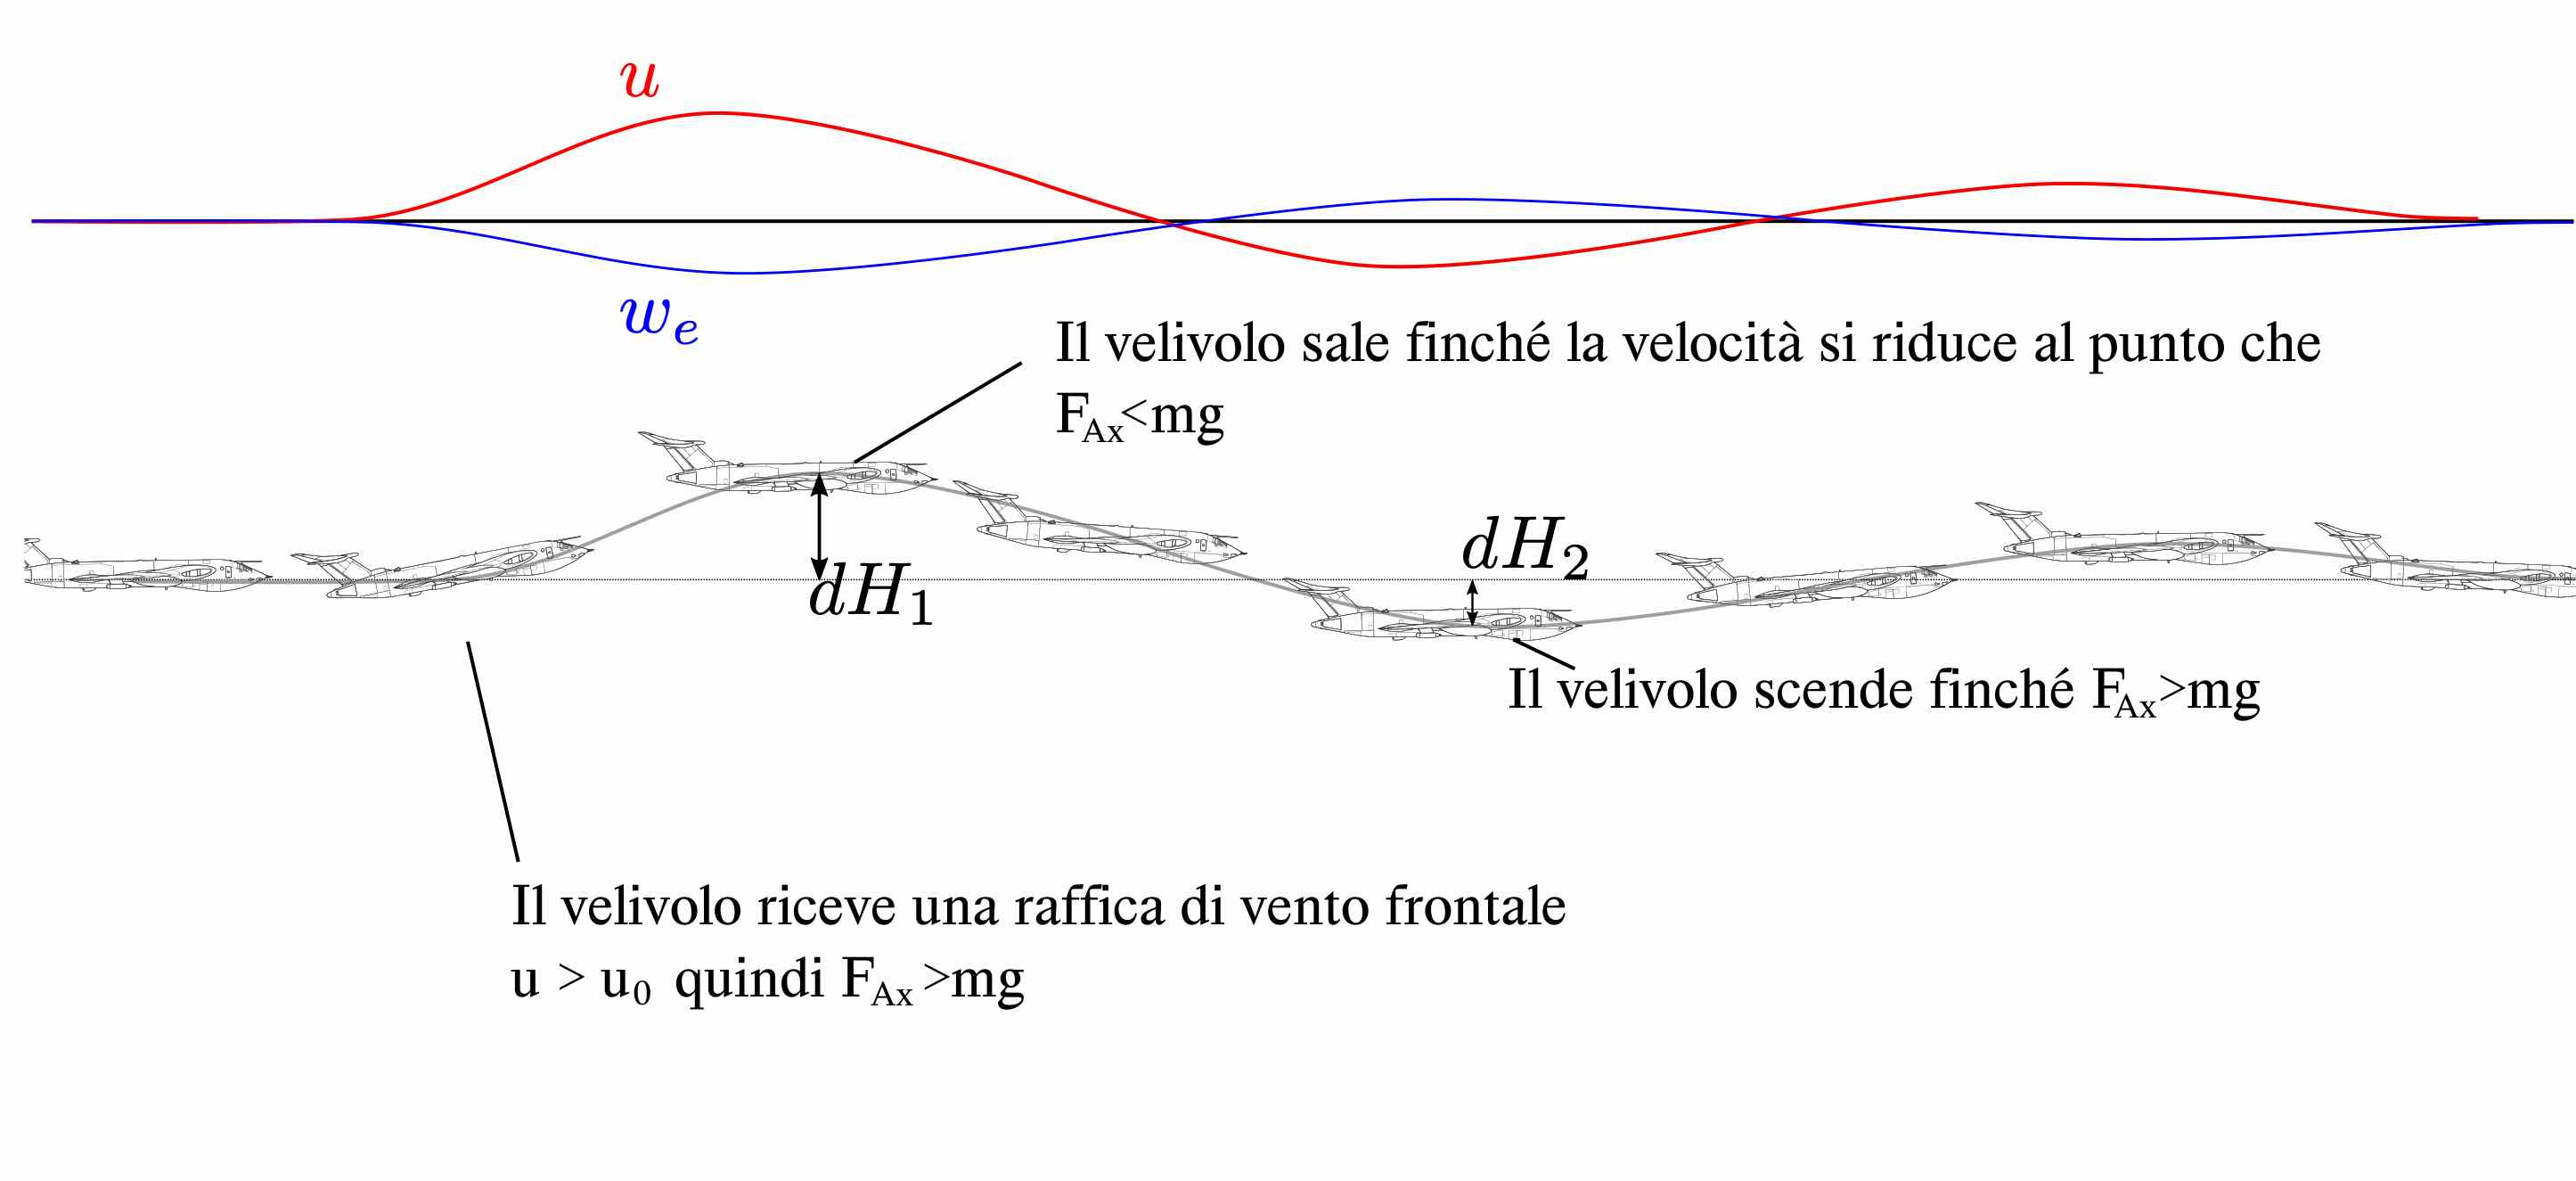
\includegraphics[width=0.9\linewidth]{Immagini/phugoid_mode_physics.jpg}
\end{figure}

In questo caso il coefficiente di smorzamento e la pulsazione naturale per i poli sono:
\begin{equation*}
    \zeta = - \frac{Re[p]}{\left|p\right|} = 0.3005 \qquad \omega_n = \left|p\right| = 0.01022rad/s
\end{equation*}

Si può notare che sia il coefficiente di smorzamento che la pulsazione naturale sono inferiori che nel modo precedente. Il tempo di assestamento è quindi molto maggiore, arrivando fino a 24 minuti per il Boeing 747 in esame.
\begin{figure}[H]
    \centering
    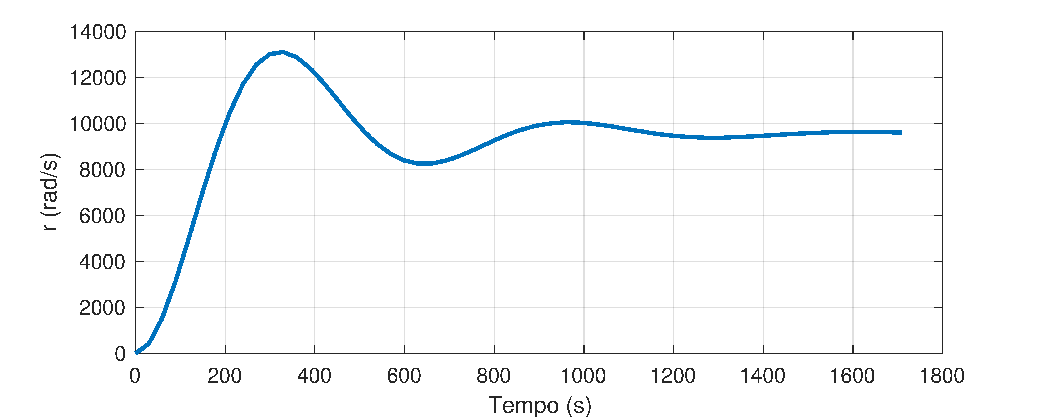
\includegraphics[width=0.7\linewidth]{Immagini/phugoid_mode.pdf}
    \caption{Risposta impulsiva dei poli associati al modo \textit{phugoid} assieme al polo nell'origine  del Boeing 747 in esame}
\end{figure}


\section{Moti Laterali}
I velivoli dotati di ali a freccia positiva, come il Boeing 747, presentano tipicamente un basso smorzamento nei modi laterali.
Tali dinamiche risultano particolarmente difficili da gestire per il pilota, motivo per cui questa tipologia di aeromobili è solitamente equipaggiata con sistemi di controllo automatico volti a supportare e facilitare il lavoro del pilota.

\subsection{Ingressi e Uscite}

I moti laterali oggetto di studio sono influenzati sia dal timone che dagli alettoni. Nel controllo verrà impiegato solamente il timone in quanto ha una maggiore autorità sui moti che si desidera ridurre.

Verrà inoltre utilizzato un giroscopio per misurare l'angolo di imbardata, in quanto particolarmente influenzato dai moti laterali.
\begin{figure}[H]
    \centering
    \begin{tikzpicture}
        \node[draw,
            circle,
            minimum size=0.5cm,
        ] (sum) at (0,0){};

        % Controller
        \node [draw,
            minimum width=2.4cm,
            minimum height=1.2cm,
            right=1.5cm of sum
        ]  (controller) {$Controllore$};

        % System
        \node [draw,
            minimum width=2.4cm,
            minimum height=2.8cm,
            right=1.5cm of controller,
            yshift=0.8cm
        ]  (system) {$Sistema$};

        % Sensor block
        \node [draw,
            minimum width=2.4cm,
            minimum height=1.2cm,
            below right= 1cm and -0.25cm of controller
        ]  (sensor) {$Giroscopio$};


        \draw[-stealth] (system.east) -- ++ (1.5,0)
        node[midway](output){}node[midway,above]{$r$};

        \draw[stealth-] (system.150) -- ++ (-1.5,0)
        node[midway,above]{$\delta_a$};

        \draw[-stealth] (controller.east) -- ++ (1.5,0);

        \draw[-stealth] (sum.east) -- ++ (1.5,0);
        \draw[stealth-] (sum.west) -- ++ (-1.25,0)
        node[midway,above]{$\delta_r$};

        \draw[-stealth] (sensor.west) -| (sum.south);

        \draw[-stealth] (output.center) |- (sensor.east);
    \end{tikzpicture}
\end{figure}

\renewcommand{\arraystretch}{1.2}
\begin{table}[H]
    \begin{tabularx}{\textwidth}{|c|X|}
        \hline
        \multicolumn{2}{|l|}{\textbf{Ingressi}}                                         \\
        \hline
        $\delta_r$ & angolo di deflessione del timone                                   \\
        \hline
        \multicolumn{2}{|l|}{\textbf{Uscite}}                                           \\
        \hline
        $r$        & componente lungo $z_{FRD}$ del vettore $\vec{w}_{FRD}$             \\
        \hline
        \multicolumn{2}{|l|}{\textbf{Variabili di Stato}}                               \\
        \hline
        $p$, $r$   & componenti lungo $x_{FRD}$ e $z_{FRD}$ del vettore $\vec{w}_{FRD}$ \\
        $\beta$    & angolo di derapata                                                 \\
        $\phi$     & angolo di rollio                                                   \\
        \hline
    \end{tabularx}
\end{table}

\subsection{Funzione di Trasferimento}
Utilizzando la funzione \texttt{ss2tf} di MATLAB sul modello di stato \eqref{eq:motoLaterale} si ottiene la funzione di trasferimento:

\begin{equation}
    \label{eq:trasferimentoLaterali}
    \begin{split}
        W_{\delta_r \rightarrow r}(s) & = \frac{-0.475 s^3 - 0.24789 s^2 - 0.11871 s - 0.056462}{s^4 + 0.6358 s^3 + 0.94078 s^2 + 0.51313 s + 0.003683} \\
                                      & = -0.475\frac{(s + 0.4987)(s + 0.0116 \pm j0.4881)}{(s + 0.5630)(s + 0.0073)(s + 0.0328 \pm j0.9478)}
    \end{split}
\end{equation}

Dalla forma di Evans \cite{zampieri_dispensa_controlli}, riportata nella seconda riga, è possibile individuare i poli e gli zeri. In particolare sono presenti tre zeri, $s = -0.4987, s = - 0.0116 \pm j0.4881$, e quattro poli, $s = -0.5630, s = -0.0073, s = -0.0328 \pm j0.9478$

\begin{figure}[H]
    \centering
    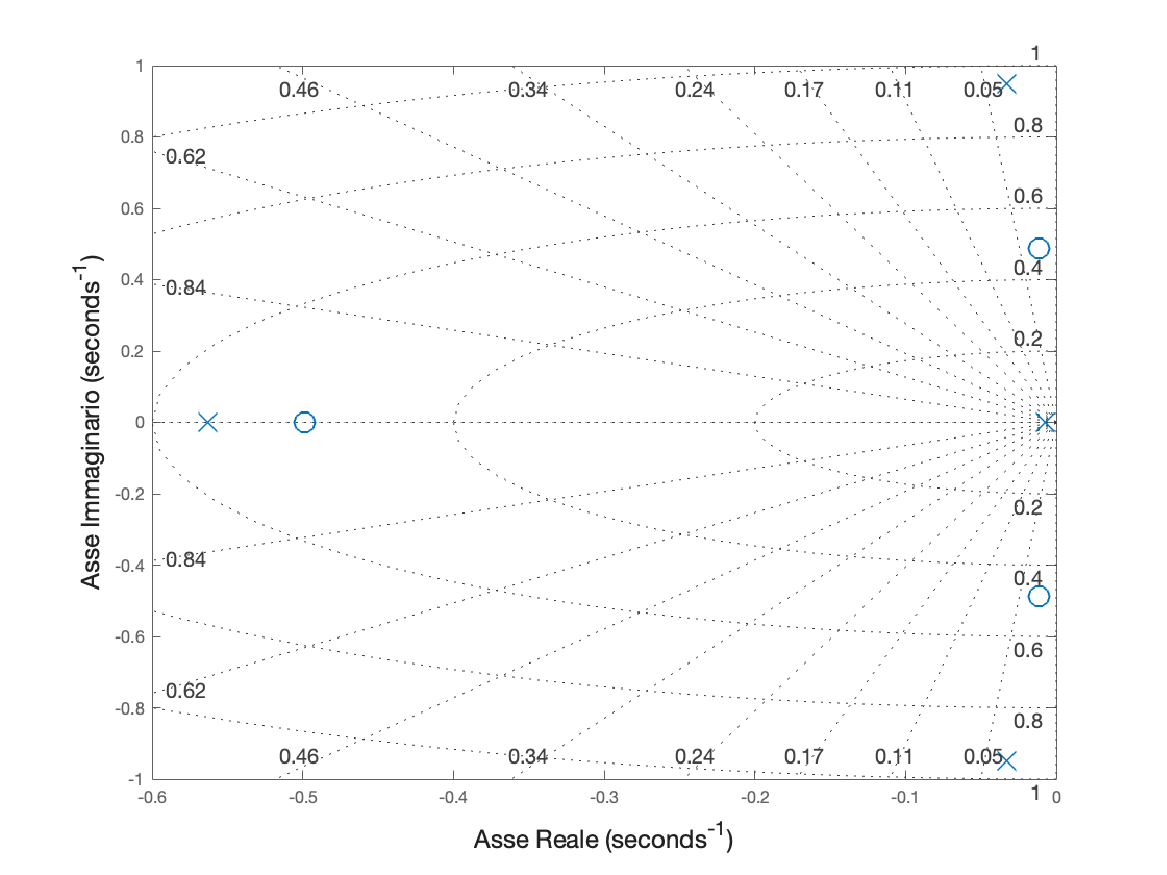
\includegraphics[width=0.7\linewidth]{Immagini/poli_laterali.pdf}
    \caption{\texttt{pzplot} dei poli e degli zeri della funzione di trasferimento $ W_{\delta_r \rightarrow r}(s)$}
\end{figure}

\subsection{Stabilità}

\subsubsection{Stabilità Rispetto alle Condizioni iniziali}

Il polinomio caratteristico del sistema è:
\begin{equation*}
    (s + 0.5630)(s + 0.0073)(s + 0.0328 \pm j0.9478)
\end{equation*}
Le sue radici hanno tutte parte reale $< 0$, è quindi possibile concludere che il sistema è asintoticamente stabile rispetto alle condizioni iniziali.

\subsubsection{BIBO Stabilità}

La funzione di trasferimento ha tutti i poli a parte reale negativa, si conclude che il sistema è BIBO stabile.

\subsection{Modi Naturali}

In questo caso la funzione di trasferimento è costituita da quattro poli: due reali e due complessi coniugati.

I poli reali danno origine a modi criticamente smorzati ($\zeta = 1$), mentre i poli complessi coniugati generano un moto oscillatorio denominato \textit{dutch roll}.

\subsubsection{Spiral}

Il modo associato al polo in $-0.0073$ è detto \textit{spiral}. Esso si manifesta quando, a seguito di una perturbazione, il velivolo acquisisce un angolo di rollio $\phi > 0$.
A seguito della perturbazione la coda del velivolo inizia a generare una componente di portanza, che tende ad aumentare ulteriormente l'angolo $\phi$.

In base all'entità della forza generata, il velivolo può ritornare lentamente alla sua posizione iniziale, come nel caso del Boeing 747, oppure può entrare in una virata di raggio decrescente che può condurre a una pericolosa situazione nota come \textit{graveyard spiral}.

\begin{figure}[H]
    \centering
    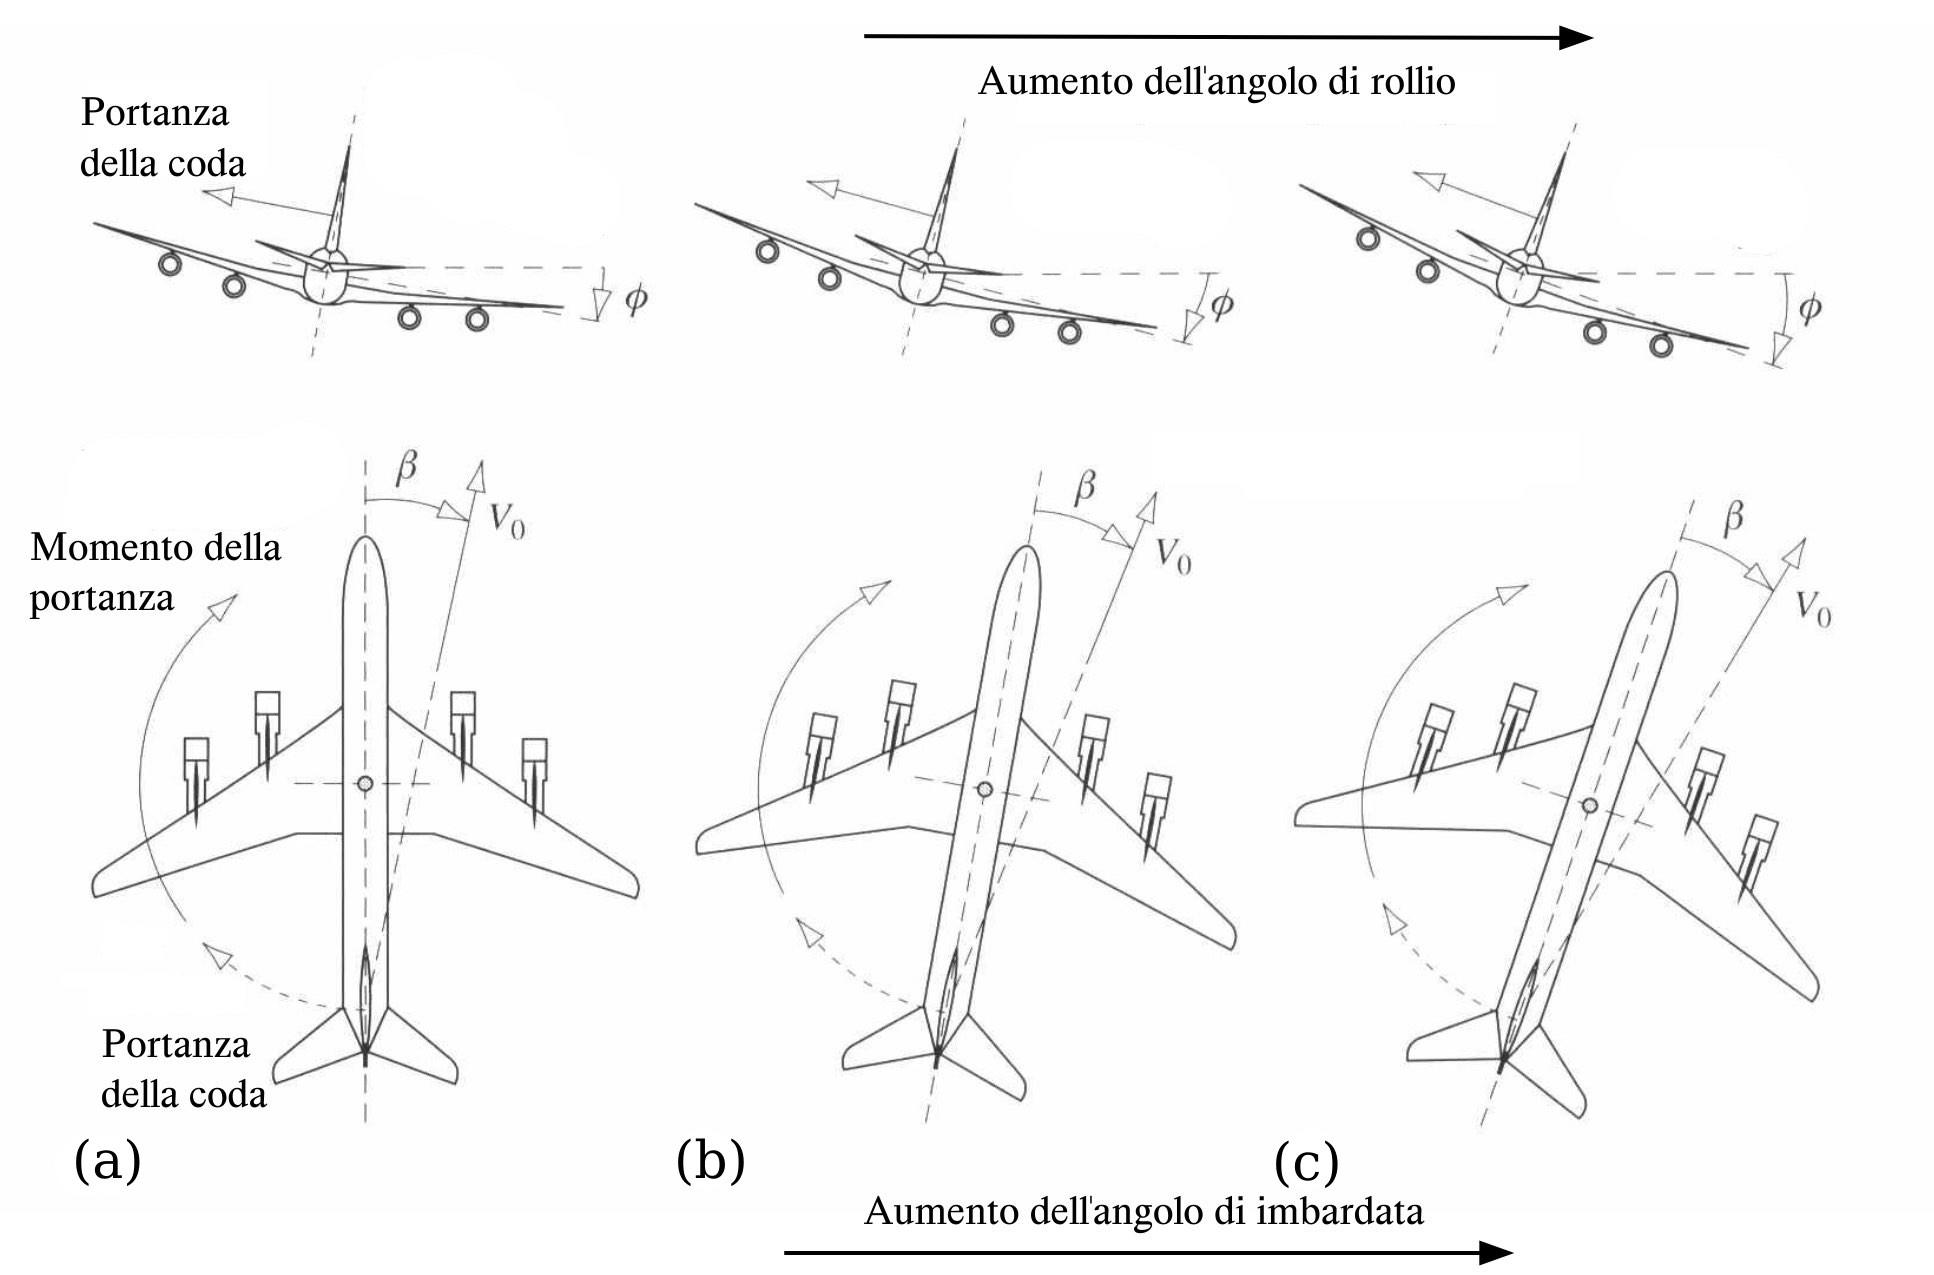
\includegraphics[width=0.8\linewidth]{Immagini/spiral_mode_physics.jpg}
    \caption{Influenza della portanza della coda sull'angolo di rollio e di imbardata \cite{cook1997flight}}
\end{figure}

Dal calcolo del coefficiente di smorzamento e della pulsazione naturale si può osservare come questo modo sia di lungo periodo:
\begin{equation*}
    \zeta = - \frac{Re[p]}{\left|p\right|} = 1 \qquad \omega_n = \left|p\right| = 0.0073rad/s
\end{equation*}

\begin{figure}[H]
    \centering
    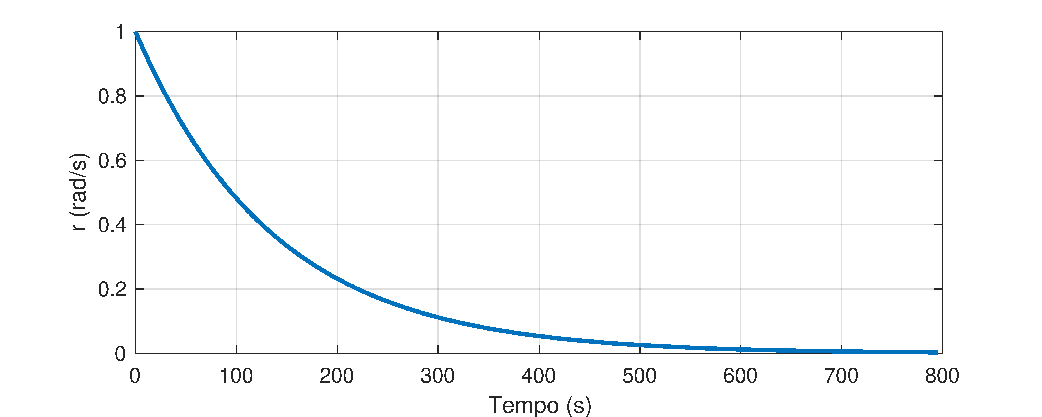
\includegraphics[width=0.7\linewidth]{Immagini/spiral_mode.pdf}
    \caption{Risposta impulsiva per il polo associato al modo \textit{spiral} del Boeing 747 in esame}
\end{figure}

\subsubsection{Roll}

Il modo associato al polo in $-0.5630$ è detto \textit{roll}. Esso si verifica quando il velivolo ruota attorno all'asse $\hat{x}_{FRD}$, ovvero quando la velocità angolare $p$ subisce una variazione.

In questo caso il modo è ben smorzato, quindi il velivolo ritorna rapidamente alla sua condizione di equilibrio dopo una perturbazione.

Ciò è confermato anche dal valore del coefficiente di smorzamento e della pulsazione naturale:
\begin{equation*}
    \zeta = - \frac{Re[p]}{\left|p\right|} = 1 \qquad \omega_n = \left|p\right| = 0.5630rad/s
\end{equation*}

\begin{figure}[H]
    \centering
    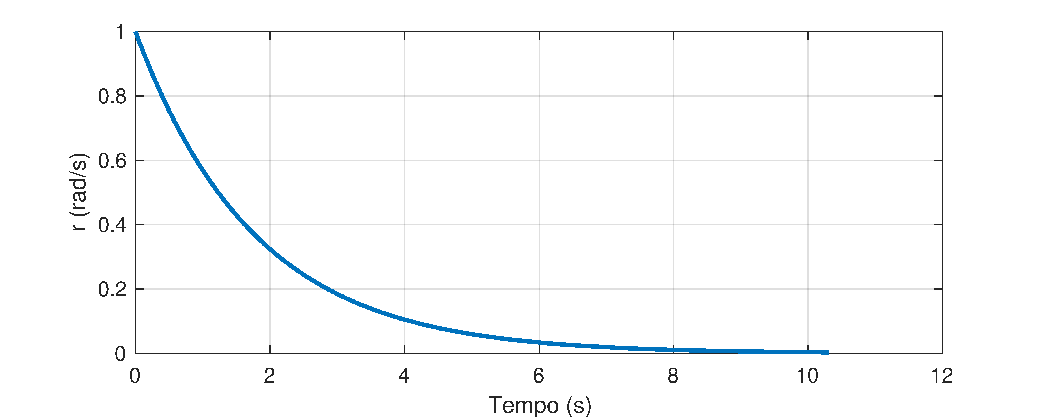
\includegraphics[width=0.7\linewidth]{Immagini/roll_mode.pdf}
    \caption{Risposta impulsiva per il polo associato al modo \textit{roll} del Boeing 747 in esame}
\end{figure}

\subsubsection{Dutch Roll}

Il modo associato ai poli in $-0.0328 \pm j0.9478$ è detto \textit{dutch roll} ed è caratterizzato da un moto oscillatorio che coinvolge simultaneamente rollio, imbardata e derapata.

In particolare, può iniziare con un incremento dell'angolo di imbardata $\psi$, che provoca una variazione dell'incidenza relativa sulle due ali: l'ala avanzata genera una maggiore portanza rispetto all'altra.
Questo squilibrio induce un aumento dell'angolo di rollio $\phi$, che a sua volta altera la direzione del moto e innesca un'imbardata in senso opposto.
Il ciclo si ripete, dando luogo a un'oscillazione di lungo periodo.

\begin{figure}[H]
    \centering
    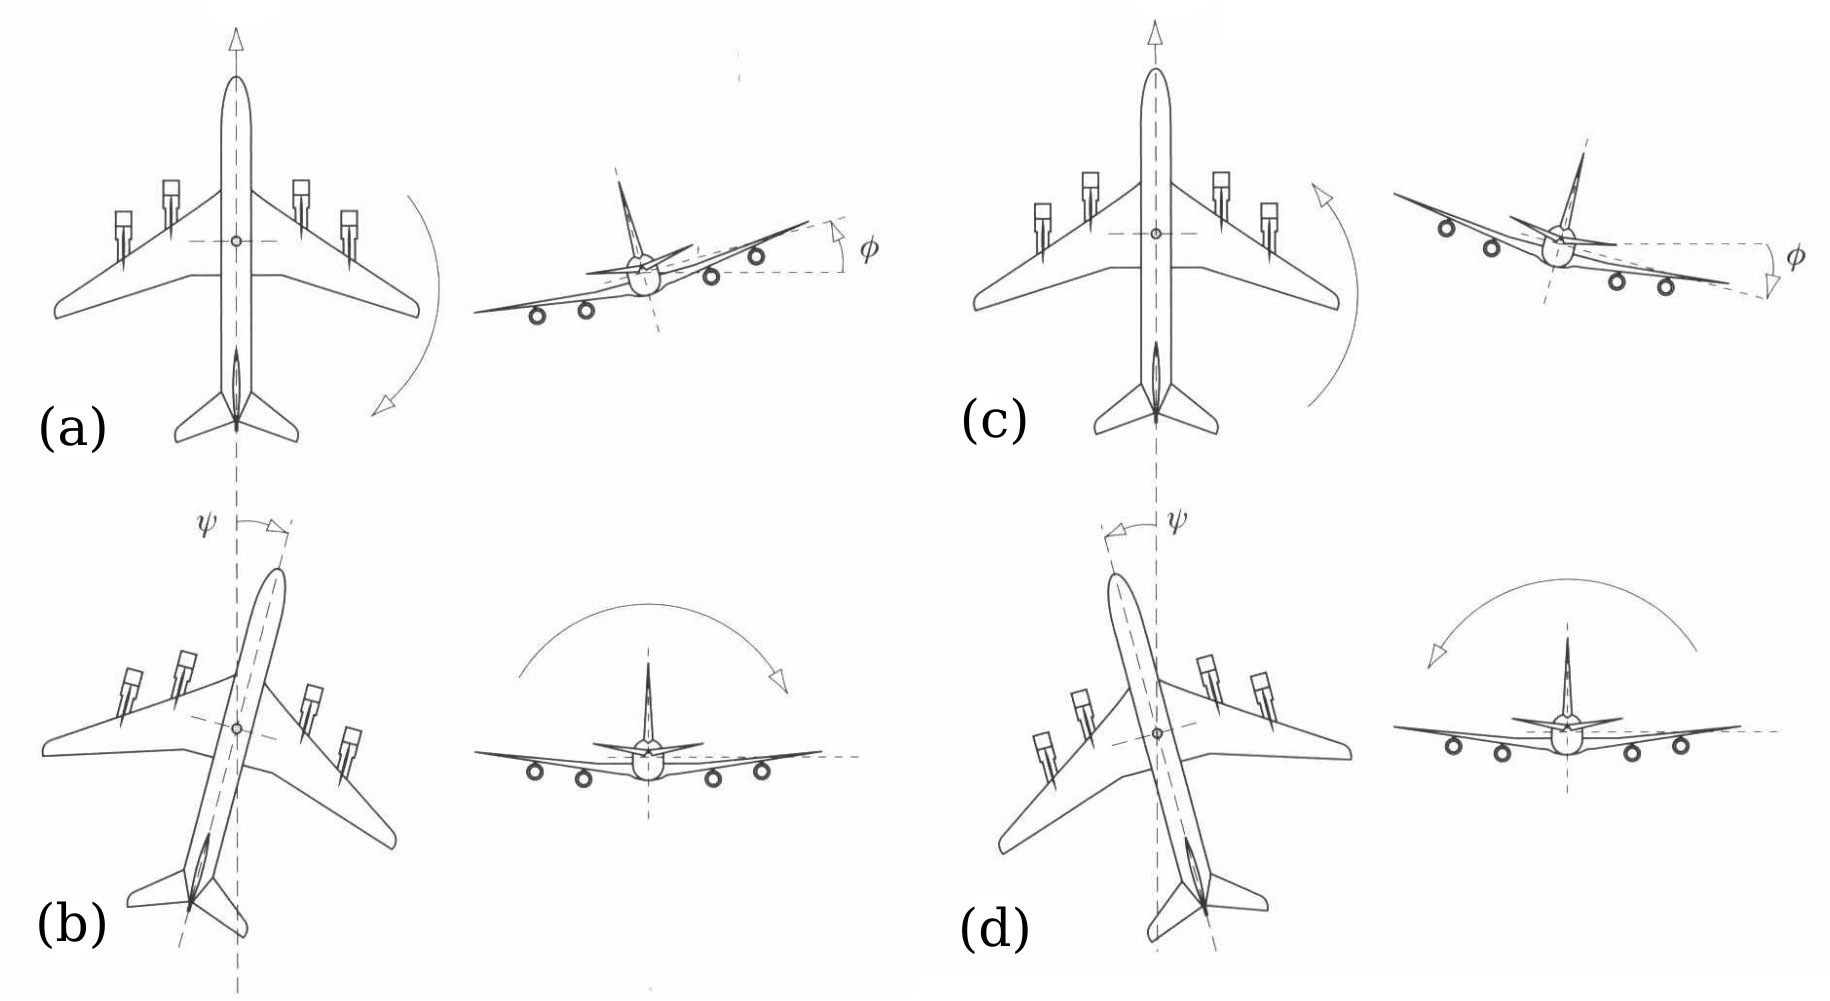
\includegraphics[width=0.8\linewidth]{Immagini/dutch_roll_physics.jpg}
    \caption{Interazione tra gli angoli di rollio e di imbardata \cite{cook1997flight}}
\end{figure}

I parametri del coefficiente di smorzamento e della pulsazione naturale sono:
\begin{equation*}
    \zeta = - \frac{Re[p]}{\left|p\right|} = 0.034585 \qquad \omega_n = \left|p\right| = 0.94836
\end{equation*}

\begin{figure}[H]
    \centering
    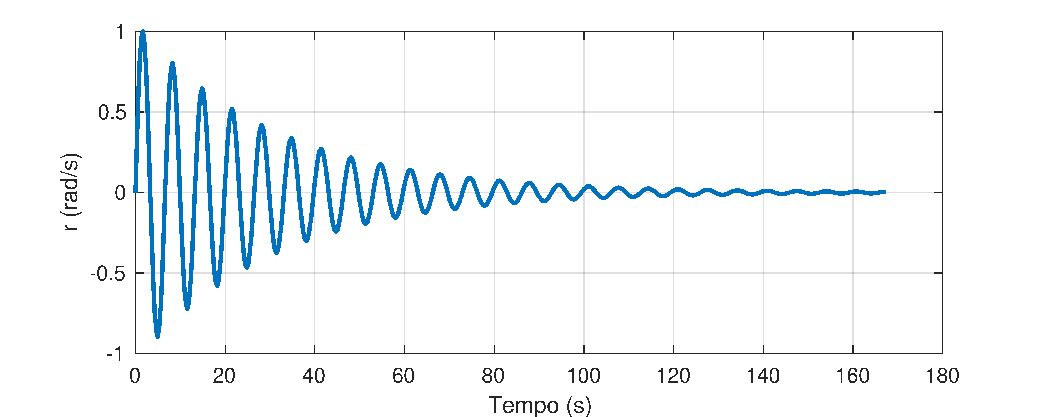
\includegraphics[width=0.7\linewidth]{Immagini/dutch_roll_mode.pdf}
    \caption{Risposta impulsiva per i poli associati al modo \textit{dutch roll} del Boeing 747 in esame}
\end{figure}


\appendix
\chapter{Report Tecnico NASA CR-2144}\label{appendix:report}
\documentclass{article}
\usepackage{float}
\usepackage[margin = 2cm]{geometry}
\usepackage{graphicx}
\usepackage{bm}
\usepackage{amsmath,amssymb,amsfonts,amsthm}
\setlength{\parindent}{0pt}

\newcommand{\spacer}[1][8pt]{
    \par\vspace{#1}
}

\author
{
    Mattia Boscolo Meneguolo - 2066700, \\
    Matteo Cuzzolin - 2066701
}
\title{Tesina di Fondamenti di Controlli Automatici, A.A. 2024}
\date{}
\begin{document}
\maketitle

\begin{figure}[!htbp]
    \centering
    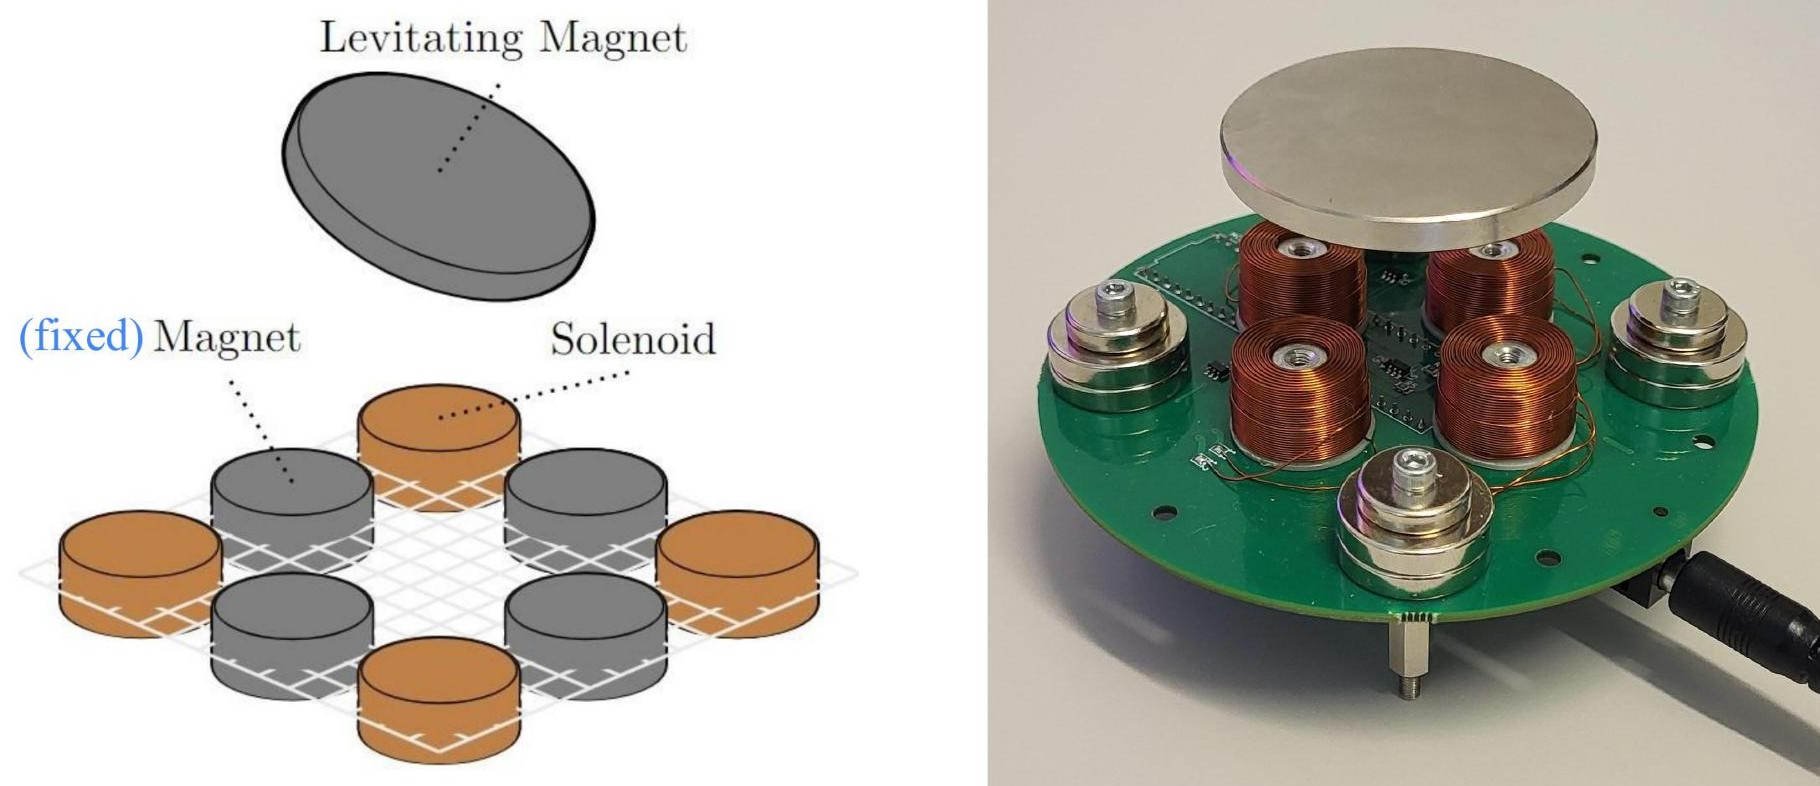
\includegraphics[width = 0.8\textwidth]{Images/maglev-system-schematics}
    \caption{Rappresentazione del sistema - Implementazione del sistema}
    \label{fig:rappresentazione_sistema}
\end{figure}

Sia $\tilde{z}(t) = z(t) - \overline{z}$ dove $z(t)$ è la posizione del magnete e $\overline{z}$ è la posizione del magnete all'equilibrio.

La trasformata di laplace di $\tilde{z}$ è:
$$\tilde{Z}(s) = \frac{b_s}{\overline{z}ms^2+\overline{z}ds+mg}I(s)+\frac{(ms+d)\tilde{z}(0)+m\tilde{z}'(0)}{ms^2+ds+\frac{mg}{\overline{z}}}$$

\section{Esercizio 1}
Studiamo la risposta libera, infatti in questo caso $i(t) = 0 \:\forall t$. Ipotizziamo anche che $\tilde{z}'(0) = 0$

$\tilde{Z}(s) =\frac{(ms+d)\tilde{z}(0)}{ms^2+ds+\frac{mg}{\overline{z}}}$

\spacer
Secondo la regola di Cartesio il polinomio al denominatore è stabile infatti tutti i coefficienti sono non nulli e positivi.

\spacer
Tuttavia dalle prime elaborazioni su mathlab risulta evidente che il sistema impiega un lungo periodo di tempo per assestarsi alla posizione di equilibrio.
Dato che vogliamo svolgere diverse simulazioni per mostrare che il sistema raggiunge l'equilibrio al variare di $\tilde{z}(0)$ aumenteremo il valore di d a 0.1 così da rendere più veloci le simulazioni.

\spacer
Questo è un esempio di una simulazione con $\tilde{z}(0)=0.35$ e $d=0.1$

\begin{figure}[H]
    \centering
    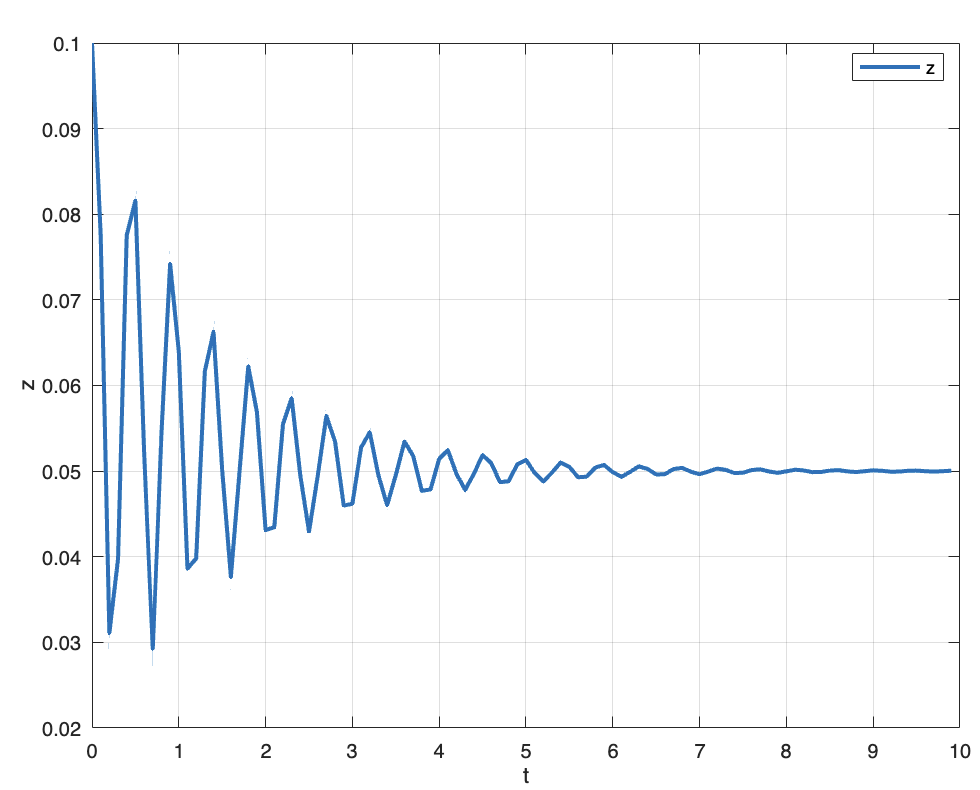
\includegraphics[width = 0.5\textwidth]{Images/simulazione-d-0.1.png}
    \caption{Simulazione $\tilde{z}(0)=0.35$}
    \label{fig:simulazione_d_0.1}
\end{figure}

\spacer
A questo punto simuliamo il sistema al variare di $\tilde{z}(0)$ e verifichiamo che dopo 10 secondi esso si assesti all'altezza di equilibrio.

\begin{figure}[H]
    \centering
    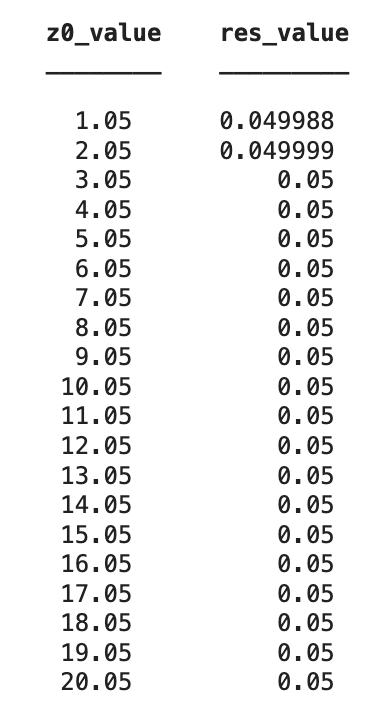
\includegraphics[width = 0.2\textwidth]{Images/risultati-simulazioni.png}
    \caption{Simulazione $\tilde{z}(0) variabile$}
    \label{fig:simulazione_z_variabile}
\end{figure}

\section{Esercizio 2}
Vogliamo disegnare il luogo delle radici della funzione di trasferimento in catena aperta del sistema, per fare questo usiamo mathlab e otteniamo:

\begin{figure}[H]
    \centering
    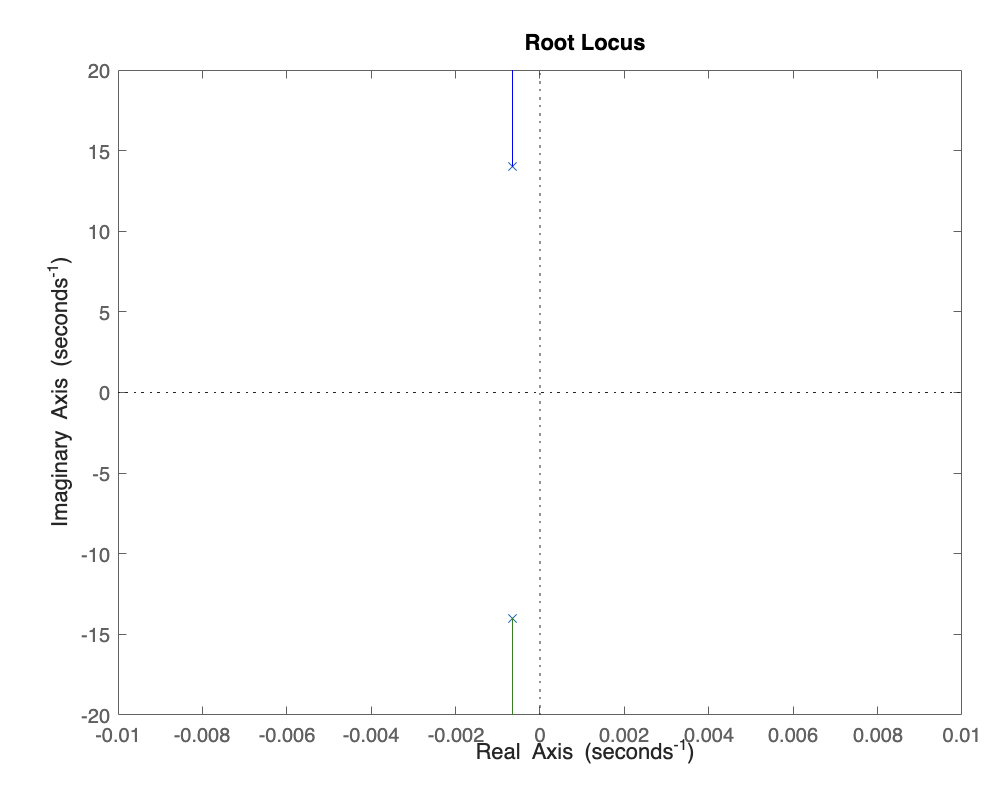
\includegraphics[width = 0.5\textwidth]{Images/luogo-radici-proporzionale.png}
    \caption{Luogo Radice in catena aperta}
    \label{fig:luogo_radice_catena_aperta}
\end{figure}

Per ottenere un controllore con un tempo di salita $T_s \le 1$ vogliamo $T_s = \frac{2}{w_n} \Rightarrow w_n = |p| = 2$

Ma le radici più vicine all'origine hanno $|p| = 14.0071$

Non è quindi possibile costruire un controllore proporzionale con i requisiti richiesti.

\section{Esercizio 3}
Scegliamo come indici di performace quelli richiesti dall'esercizio precedente, ovvero 1 secondo di settling time, quindi anche il tempo di salita deve essere inferiore al secondo.
Inoltre cerchiamo un controllore che abbia la minima sovraelongazione.

\spacer
Abbiamo prima utilizzato un noto metodo euristico, detto Ziegler-Nichols. Seguendo il semplice algoritmo abbiamo ottenuto i seguenti valori del controllore:

$K_p = 8.4028;$

$K_i = 10.1198;$

$K_d = 0.37896;$

\spacer
Ottenendo così il seguente risultato:

\begin{figure}[H]
    \centering
    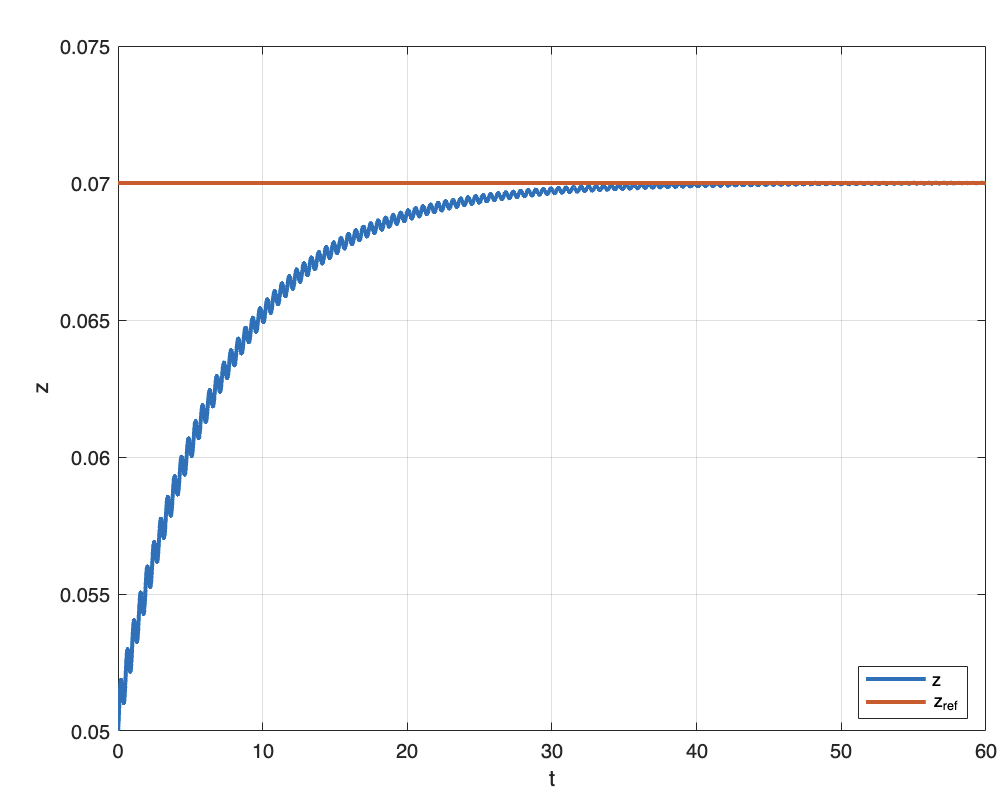
\includegraphics[width = 0.5\textwidth]{Images/PID-euristico.png}
    \caption{Sistema controllato con PID ottenuto con il metodo Ziegler-Nichols}
    \label{fig:Ziegler_Nichols_PID}
\end{figure}

Questo controllore non soddisfa le nostre richieste in quanto impiega circa 40 secondi a raggiungere il regime, tuttavia non presenta alcuna sovraelongazione.

\spacer
Per trovare un controllore con prestazioni migliori abbiamo utilizzato la funzione \texttt{pidTuner} di Mathlab.

Utilizzando i valori restituiti dal tuner, ovvero:

$K_p = 8.9131;$

$K_i = 52.4269;$

$K_d = 0.37883;$

\spacer
Ottenendo così il seguente risultato:

\begin{figure}[H]
    \centering
    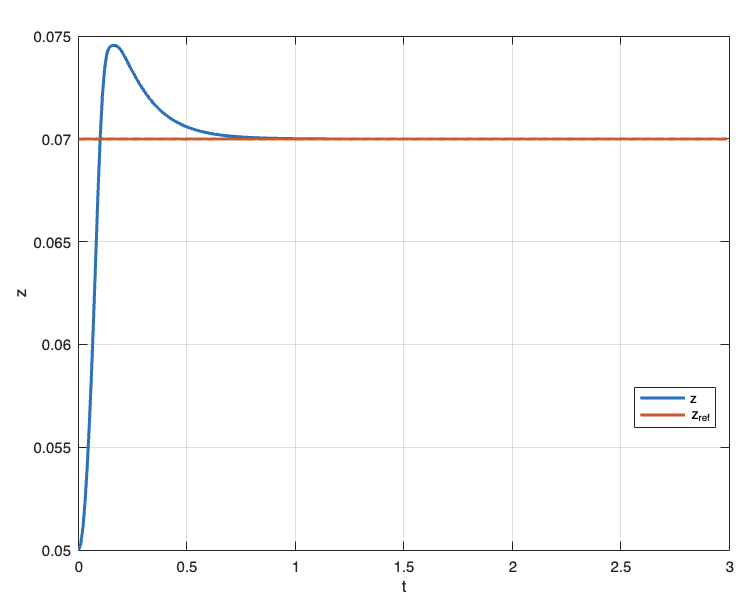
\includegraphics[width = 0.5\textwidth]{Images/PID-tuner.png}
    \caption{Sistema controllato con PID ottenuto con pidTuner}
    \label{fig:pidTuner-PID}
\end{figure}

Il controllore ottenuto è di gran lunga migliore e soddisfa i requisiti che ci eravamo posti, porta il sistema a regime in poco meno di un secondo tuttavia ha una sovraelongazione importante.

\spacer
Infine abbiamo voluto cercare un controllore con una minore sovraelongazione, ignorando il limite di tempo.

Utilizzando i seguenti valori:

$K_p = 7.2786;$

$K_i = 14.8316;$

$K_d = 0.89298;$

\spacer
Ottenendo così il seguente risultato:

\begin{figure}[H]
    \centering
    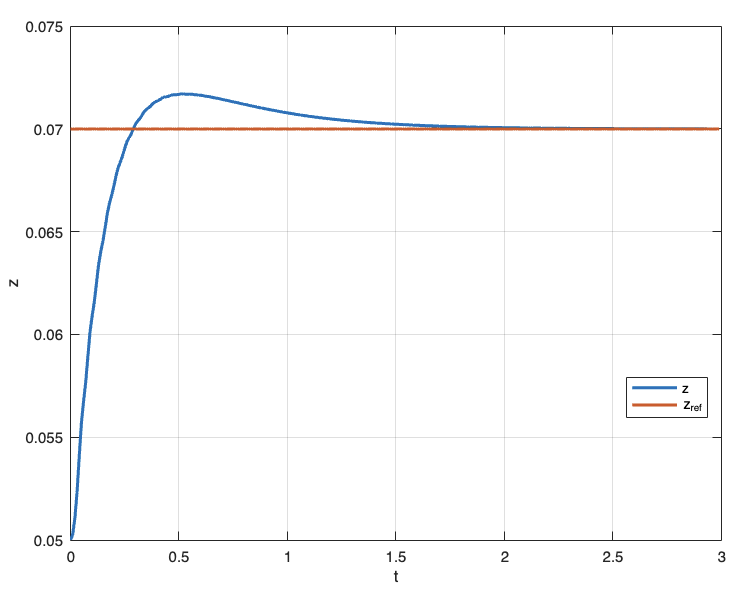
\includegraphics[width = 0.5\textwidth]{Images/PID-tuner-overshoot.png}
    \caption{Sistema controllato con PID ottenuto con pidTuner con richieste modificate}
    \label{fig:pidTuner-PID-overshoot}
\end{figure}

\section{Esercizio 4}
Per verificare l'altezza massima che il magnete è in grado di raggiungere utilizziamo un controllore instabile, trovato durante il nostro lavoro di ricerca dell'esercizio 2, in particolare un controllore proporzionale con $K = 1$.

Otteniamo poi il valore massimo simulando l'evoluzione del sistema e prendendo il valore massimo.

\begin{figure}[H]
    \centering
    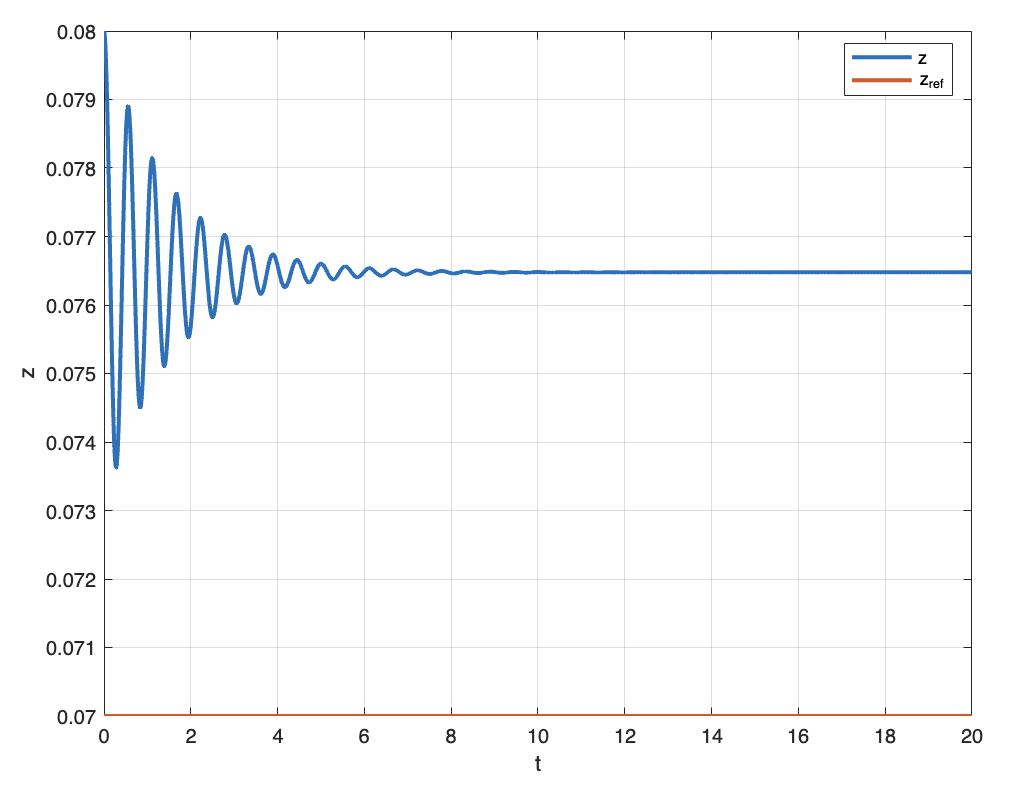
\includegraphics[width = 0.5\textwidth]{Images/max-z.png}
    \caption{Sistema controllato con controllore instabile}
    \label{fig:max-z}
\end{figure}

Vediamo sperimentalmente che il valore massimo a regime che il sistema può raggiungere è $0.25213$.

\section{Esercizio 5}
Per far seguire al magnete i segnali di riferimento richiesti abbiamo utilizzato in entrambi i casi un controllore PID con valori modificati per adattarsi meglio al problema.

\spacer
Nel caso del riferimento sinusoidale abbiamo utilizzato il controllore fornito dal tuner di mathlab:

$K_p = 8.9131;$

$K_i = 52.4269;$

$K_d = 0.37883;$

\begin{figure}[H]
    \centering
    \begin{minipage}{0.45\textwidth}
        \begin{figure}[H]
            \centering
            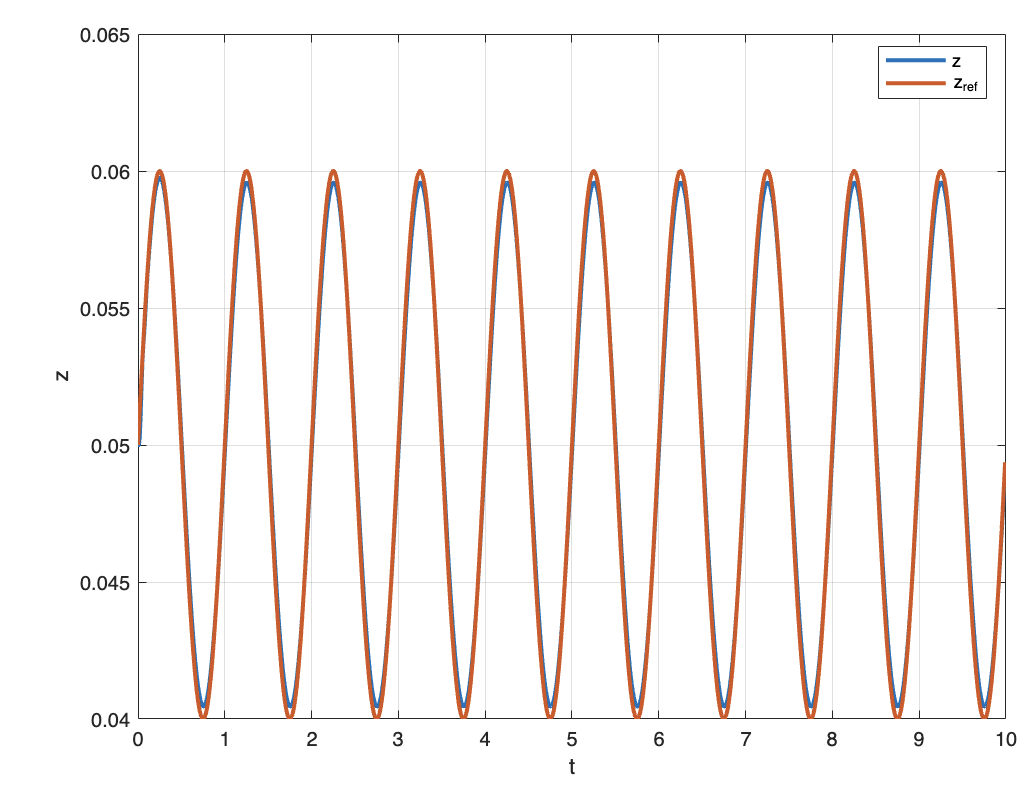
\includegraphics[width = 1\textwidth]{Images/sine.png}
            \caption{Sistema controllato con controllore PID}
            \label{fig:PID-sine}
        \end{figure}
    \end{minipage}
    \hfill
    \begin{minipage}{0.45\textwidth}
        \begin{figure}[H]
            \centering
            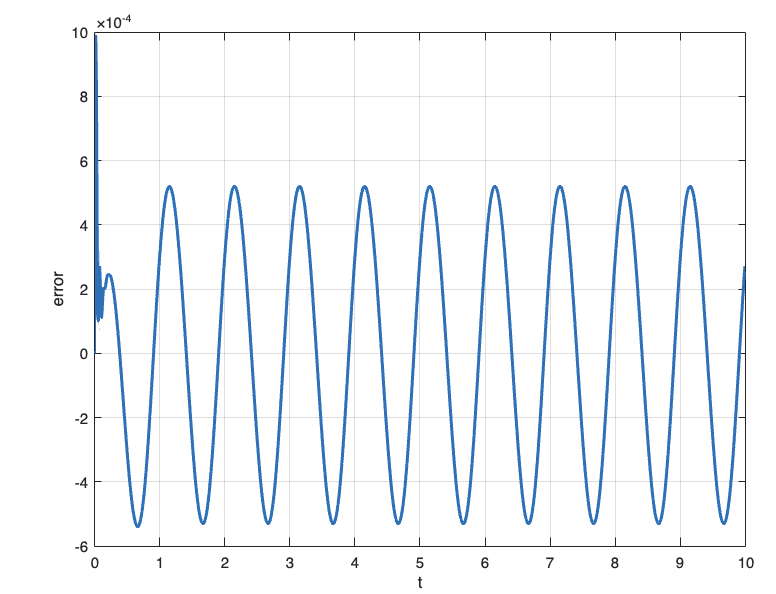
\includegraphics[width = 1\textwidth]{Images/sine-error.png}
            \caption{Errore del sistema}
            \label{fig:PID-sine-error}
        \end{figure}
    \end{minipage}
\end{figure}

\spacer
Nel caso del riferimento ad onda quadra abbiamo utilizzato dei valori forniti dal tuner, ma leggermente modificati:

$K_p = 8.4028;$

$K_i = 10.1198;$

$K_d = 0.37896;$

\begin{figure}[H]
    \centering
    \begin{minipage}{0.45\textwidth}
        \begin{figure}[H]
            \centering
            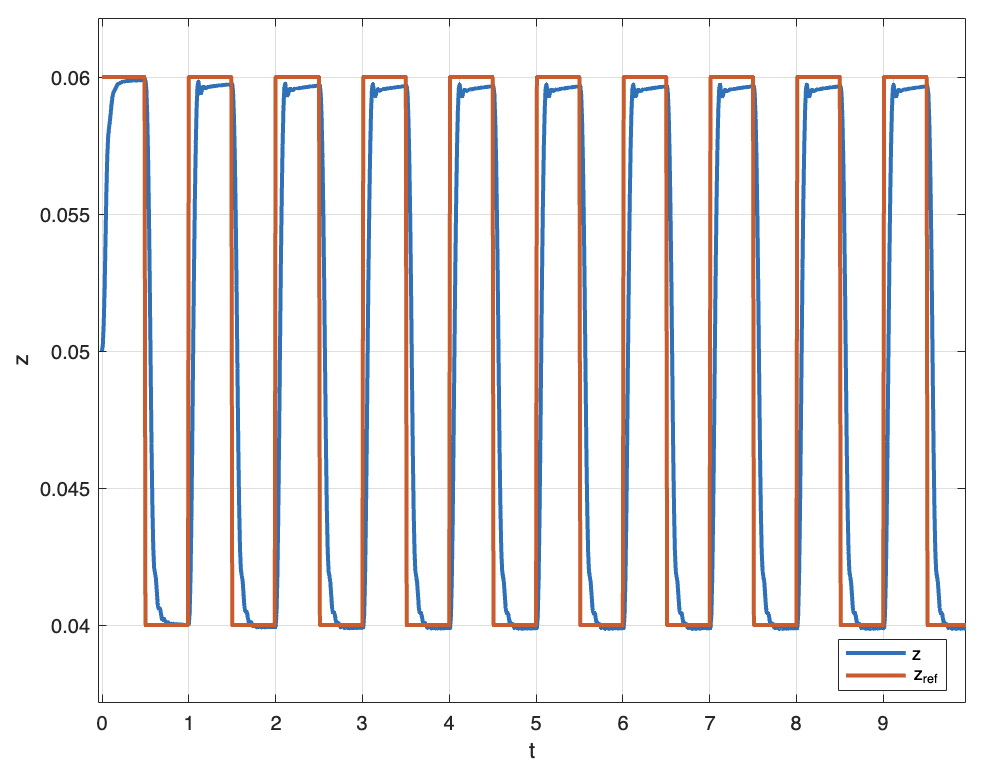
\includegraphics[width = 1\textwidth]{Images/square.png}
            \caption{Sistema controllato con controllore PID}
            \label{fig:PID-square}
        \end{figure}
    \end{minipage}
    \hfill
    \begin{minipage}{0.45\textwidth}
        \begin{figure}[H]
            \centering
            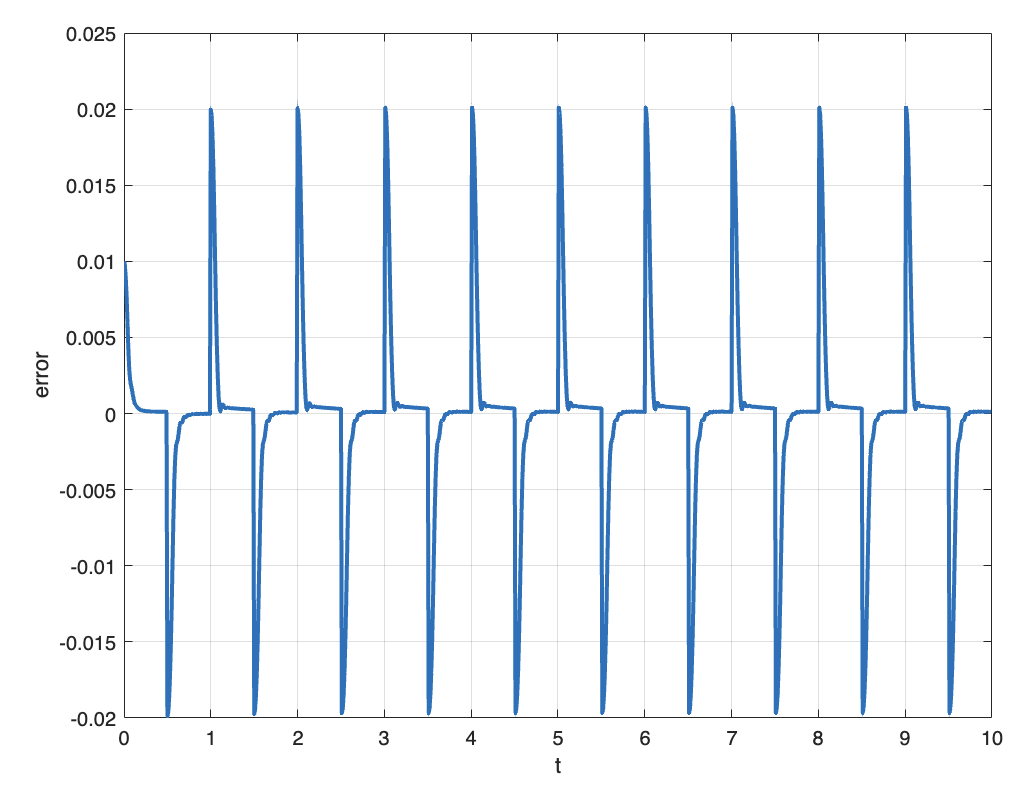
\includegraphics[width = 1\textwidth]{Images/square-error.png}
            \caption{Errore del sistema}
            \label{fig:PID-square-error}
        \end{figure}
    \end{minipage}
\end{figure}

In entrambi i casi il magnete segue accuratamente il segnale di riferimento, all'interno dei requisiti posti dal problema.

\end{document}


\cleardoublepage

\printbibliography[heading=bibintoc]
\end{document}
